% !TeX encoding = UTF-8
% !TeX program = xelatex
% !TeX spellcheck = en_US

\documentclass[degree=master]{thuthesis}
  % 学位 degree:
  %   doctor | master | bachelor | postdoc
  % 学位类型 degree-type:
  %   academic(默认)| professional
  % 语言 language
  %   chinese(默认)| english
  % 字体库 fontset
  %   windows | mac | fandol | ubuntu
  % 研究生院建议终版使用 Windows 平台的字体编译


% 论文基本配置,加载宏包等全局配置
% !TeX root = ./thuthesis-example.tex

% 论文基本信息配置

\thusetup{
  %******************************
  % 注意:
  %   1. 配置里面不要出现空行
  %   2. 不需要的配置信息可以删除
  %   3. 建议先阅读文档中所有关于选项的说明
  %******************************
  %
  % 输出格式
  %   选择打印版(print)或用于提交的电子版(electronic),前者会插入空白页以便直接双面打印
  %
  output = print,
  %
  % 标题
  %   可使用“\\”命令手动控制换行
  %
  title  = {保护隐私的卷积神经网络\\遗忘方法研究},
  title* = {Research on the Forgetting Method of Convolutional Neural Network\\ to Protect Privacy},
  %
  % 学位
  %   1. 学术型
  %      - 中文
  %        需注明所属的学科门类,例如:
  %        哲学、经济学、法学、教育学、文学、历史学、理学、工学、农学、医学、
  %        军事学、管理学、艺术学
  %      - 英文
  %        博士:Doctor of Philosophy
  %        硕士:
  %          哲学、文学、历史学、法学、教育学、艺术学门类,公共管理学科
  %          填写“Master of Arts“,其它填写“Master of Science”
  %   2. 专业型
  %      直接填写专业学位的名称,例如:
  %      教育博士、工程硕士等
  %      Doctor of Education, Master of Engineering
  %   3. 本科生不需要填写
  %
  degree-name  = {工程硕士},
  degree-name* = {Master of Engineering},
  %
  % 培养单位
  %   填写所属院系的全名
  %
  department = {软件学院},
  %
  % 学科
  %   1. 学术型学位
  %      获得一级学科授权的学科填写一级学科名称,其他填写二级学科名称
  %   2. 工程硕士
  %      工程领域名称
  %   3. 其他专业型学位
  %      不填写此项
  %   4. 本科生填写专业名称,第二学位论文需标注“(第二学位)”
  %
  discipline  = {软件工程},
  discipline* = {Software Engineering},
  %
  % 姓名
  %
  author  = {潘海楠},
  author* = {Pan Hainan},
  %
  % 指导教师
  %   中文姓名和职称之间以英文逗号“,”分开,下同
  %
  supervisor  = {刘云浩, 教授},
  supervisor* = {Professor Liu Yunhao},
  %
  % 副指导教师
  %
  % associate-supervisor  = {丁旋, 助理研究员},
  % associate-supervisor* = {Professor Ding Xuan},
  %
  % 联合指导教师
  %
  % co-supervisor  = {丁旋, 助理研究员},
  % co-supervisor* = {Assistant Researcher Ding Xuan},
  %
  % 日期
  %   使用 ISO 格式;默认为当前时间
  %
  date = {2021-05-18},
  %
  % 是否在中文封面后的空白页生成书脊(默认 false)
  %
  include-spine = true,
  %
  % 密级和年限
  %   秘密, 机密, 绝密
  %
  % secret-level = {秘密},
  % secret-year  = {10},
  %
  % 博士后专有部分
  %
  % clc                = {分类号},
  % udc                = {UDC},
  % id                 = {编号},
  % discipline-level-1 = {计算机科学与技术},  % 流动站(一级学科)名称
  % discipline-level-2 = {系统结构},          % 专业(二级学科)名称
  % start-date         = {2011-07-01},        % 研究工作起始时间
}

% 载入所需的宏包

% 定理类环境宏包
\usepackage{amsthm}
% 也可以使用 ntheorem
% \usepackage[amsmath,thmmarks,hyperref]{ntheorem}

\thusetup{
  %
  % 数学字体
  % math-style = GB,  % GB | ISO | TeX
  math-font  = xits,  % sitx | xits | libertinus
}

% 可以使用 nomencl 生成符号和缩略语说明
% \usepackage{nomencl}
% \makenomenclature

% 表格加脚注
\usepackage{threeparttable}

% 表格中支持跨行
\usepackage{multirow}

% 固定宽度的表格。
% \usepackage{tabularx}

% 跨页表格
\usepackage{longtable}

% 量和单位
\usepackage{siunitx}

% 参考文献使用 BibTeX + natbib 宏包
% 顺序编码制
\usepackage[sort]{natbib}
\bibliographystyle{thuthesis-numeric}

% 著者-出版年制
% \usepackage{natbib}
% \bibliographystyle{thuthesis-author-year}

% 本科生参考文献的著录格式
% \usepackage[sort]{natbib}
% \bibliographystyle{thuthesis-bachelor}

% 参考文献使用 BibLaTeX 宏包
% \usepackage[backend=biber,style=thuthesis-numeric]{biblatex}
% \usepackage[backend=biber,style=thuthesis-author-year]{biblatex}
% \usepackage[backend=biber,style=apa]{biblatex}
% \usepackage[backend=biber,style=mla-new]{biblatex}
% 声明 BibLaTeX 的数据库
% \addbibresource{ref/refs.bib}

% 定义所有的图片文件在 figures 子目录下
\graphicspath{{figures/}}

% 数学命令
\makeatletter
\newcommand\dif{%  % 微分符号
  \mathop{}\!%
  \ifthu@math@style@TeX
    d%
  \else
    \mathrm{d}%
  \fi
}
\makeatother

% hyperref 宏包在最后调用
\usepackage{hyperref}



\begin{document}

% 封面
\maketitle

% 学位论文指导小组、公开评阅人和答辩委员会名单
% !TeX root = ../thuthesis-example.tex

\begin{committee}[name={学位论文指导小组、公开评阅人和答辩委员会名单}]

  \newcolumntype{C}[1]{@{}>{\centering\arraybackslash}p{#1}}

  % \section*{指导小组名单}

  % \begin{center}
  %   \begin{tabular}{C{3cm}C{3cm}C{9cm}@{}}
  %     李XX & 教授     & 清华大学 \\
  %     王XX & 副教授   & 清华大学 \\
  %     张XX & 助理教授 & 清华大学 \\
  %   \end{tabular}
  % \end{center}


  \section*{公开评阅人名单}

  \begin{center}
    \begin{tabular}{C{3cm}C{3cm}C{9cm}@{}}
      刘XX & 教授   & 清华大学                    \\
      陈XX & 副教授 & XXXX大学                    \\
      杨XX & 研究员 & 中国XXXX科学院XXXXXXX研究所 \\
    \end{tabular}
  \end{center}


  \section*{答辩委员会名单}

  \begin{center}
    \begin{tabular}{C{2.75cm}C{2.98cm}C{4.63cm}C{4.63cm}@{}}
      主席 & 赵XX                  & 教授                    & 清华大学       \\
      委员 & 刘XX                  & 教授                    & 清华大学       \\
          & \multirow{2}{*}{杨XX} & \multirow{2}{*}{研究员} & 中国XXXX科学院 \\
          &                       &                         & XXXXXXX研究所  \\
          & 黄XX                  & 教授                    & XXXX大学       \\
          & 周XX                  & 副教授                  & XXXX大学       \\
      秘书 & 吴XX                  & 助理研究员              & 清华大学       \\
    \end{tabular}
  \end{center}

\end{committee}



% 也可以导入 Word 版转的 PDF 文件
% \begin{committee}[file=figures/committee.pdf]
% \end{committee}


% 使用授权的说明
\copyrightpage
% 将签字扫描后授权文件 scan-copyright.pdf 替换原始页面
% \copyrightpage[file=scan-copyright.pdf]

\frontmatter
% !TeX root = ../thuthesis-example.tex

% 中英文摘要和关键字

\begin{abstract}

  当今以人脸识别、自然语言处理为代表的人工智能技术被广泛应用于社会的各个领域。越来越多的个人数据被用来训练模型的同时,个人隐私泄露问题也逐渐浮出水面。
  有研究表明\cite{10.5555/3241094.3241142,Fredrikson2015},仅通过神经网络的模型参数就能还原用于训练模型的数据信息。
  为了防止自己的隐私泄露,当人们不再使用该服务时,希望模型能够“忘记”自己提供过的数据。可是现在的机器学习模型的遗忘方法没有成熟的理论。
  欧盟等国家为了更好地保护公民的个人隐私而颁布了《通用数据保护条例(GDPR)》,这为机器学习模型遗忘方法的研究增加了一定的紧迫性。
  当前具有代表性的相关工作通常使用分割网络式重新训练或使用增加噪音的方法来进行遗忘。分割网络式重新训练方法的模型会造成大量的参数存储,而增加噪音的遗忘方法仍然会使用保留数据来训练全部网络,网络的收敛时间无法得到保证。
  本文从卷积神经网络的分层抽象特性出发,专注研究如何使得卷积神经网络的机器学习模型快速且有效地忘记训练数据,提出了只训练部分参数就能达到理想遗忘效果的遗忘方案,该方案能够适用于所有使用卷积神经网络训练的模型。
  卷积神经网络自身的设计结构导致较低层次的参数提取的是和输入信息联系比较密切的基础信息,较高层次的参数提取的是和分类密切相关的特征。所以我们只需要重置和分类密切相关的参数就能达到理想的遗忘效果。
  该方案可以大致分为三个步骤:确定重置层数,冻结并重置参数和再训练网络。为了评价遗忘效果,我们引用了三个评价指标,分别是测试准确率、收敛时间和激活距离。
  
  为了检验本文遗忘方法的有效性,我们设计了四个实验来进行验证,分别是确定冻结层数实验,冻结必要性验证实验,反向冻结验证实验和遗忘可持续性验证实验。
  实验结果表明,本文提出的方法可以在不损失保留类别准确率的条件下达到理想的遗忘效果。
  通过与完全重新训练后的网络进行对比,我们发现两个网络在输出上能够达到足够的相似,而且本文的遗忘方法在收敛时间上与完全重新训练的时间相比能够缩短一半以上。
  我们还对本文遗忘方法重复使用的情况进行了实验验证。实验结果表明,本文的遗忘方法可以用于连续性的遗忘操作而不会降低遗忘效果。

  % 关键词用“英文逗号”分隔,输出时会自动处理为正确的分隔符
  \thusetup{
    keywords = {隐私保护, 遗忘, 卷积神经网络},
  }
\end{abstract}

\begin{abstract*}
  Today, artificial intelligence technologies represented by face recognition and natural language processing are widely used in various fields of society. 
  As more and more personal data are used to train models, the problem of personal privacy leakage has gradually surfaced.
  Studies\cite{10.5555/3241094.3241142,Fredrikson2015} have shown that only the model parameters of the neural network can restore the data information used to train the model.
  In order to prevent their privacy from leaking, when people no longer use the service, it is hoped that the model can "forget" the data they have provided. 
  However, the current forgetting method of machine learning models has no mature theory.
  The European Union and other countries have formulated the "General Data Protection Regulation (GDPR)" in order to better protect the personal privacy of citizens. 
  This is an increase in the urgency of the study of machine learning model forgetting methods.
  Existing representative related work is the use of segmentation network retraining or the use of noise-increasing methods for forgetting. 
  The model of the split network retraining method will cause a large amount of parameter storage, and the forgetting method of increasing noise will still use the reserved data to train the entire network, 
  and the convergence time of the network cannot be guaranteed.
  Starting from the hierarchical abstract characteristics of convolutional neural networks, 
  this paper focuses on how to make the machine learning model of convolutional neural networks forget the training data quickly and effectively, 
  and proposes a forgetting scheme that can achieve the ideal forgetting effect by training only part of the parameters. 
  The solution can be applied to all models trained using convolutional neural networks.
  The design structure of the convolutional neural network itself causes the lower-level parameters to extract basic information that is more closely related to the input information, 
  and the higher-level parameters to extract features that are closely related to classification.
  So we only need to reset the parameters closely related to the classification to achieve the desired forgetting effect.
  The scheme can be roughly divided into three steps: determining the number of reset layers, freezing and resetting parameters, and retraining the network. 
  In order to evaluate the effect of forgetting, we quoted three evaluation indicators, namely test accuracy, convergence time and activation distance.
  
  In order to test the effectiveness of the forgetting method in this paper, we designed four experiments for verification, 
  namely, the determination of the freezing layer number, the freezing necessity verification experiment, the reverse freezing verification experiment and the forgetting sustainability verification experiment.
  The experimental results show that the method proposed in this paper can achieve the ideal forgetting effect without losing the accuracy of the retention category.
  By comparing with the completely retrained network, we found that the two networks can achieve sufficient similarity in output, 
  and the forgetting method in this paper can shorten the convergence time by more than half compared with the time of complete retraining.
  We also conducted experiments to verify the repeated use of the forgetting method in this paper. 
  Experimental results show that the forgetting method in this paper can be used for continuous forgetting operations without reducing the forgetting effect.

  % Use comma as seperator when inputting
  \thusetup{
    keywords* = {Privacy Preserving, Forgetting, Convolutional Neural Network},
  }
\end{abstract*}


% 目录
\tableofcontents

% 插图和附表清单
% 本科生的插图索引和表格索引需要移至正文之后、参考文献前
\listoffiguresandtables  % 插图和附表清单
% \listoffigures           % 插图清单
% \listoftables            % 附表清单

% 符号对照表
% !TeX root = ../thuthesis-example.tex

\begin{denotation}[3cm]
  \item[GDPR] 欧盟于2018年5月25日正式施行的《通用数据保护条例》
  \item[CCPA] 美国《加州消费者隐私法案(California Consumer Privacy Act)》 
  \item[PCA] Principal components analysis,主成分分析法
  \item[SVM] Support Vector Machine,支持向量机
  \item[CNN] Convolutional Neural Network,卷积神经网络
  \item[LFW] Labled Faces in the Wild,人脸数据集
  \item[API] Application Programming Interface,应用程序接口
  \item[k-means] 一种计算机聚类算法
  \item[Fine-Tuning] 一种神经网络训练方法,俗称微调
  \item[ReLU] 神经网络的一种非线性激活函数
  \item[Sigmoid] 神经网络的一种非线性激活函数
  \item[Affine] 仿射转换,对向量做空间平移的操作
  \item[Softmax] 一种数学计算公式,将有限项离散概率分布的梯度对数归一化
  \item[MNIST] Mixed National Institute of Standards and Technology database,是美国国家标准与技术研究院收集整理的大型手写数字数据库
  \item[CIFAR-10] 是一个用于识别普适物体的小型数据集,有10个类别,每个类别有6000个图像
  \item[LEARNING\_RATE] 学习率超参数
  \item[WEIGHT\_DECAY] 权重衰减超参数
  \item[MOMENTUM] 训练冲量超参数  
  \item[BATCH\_SIZE] 每次训练迭代使用的训练数据的个数
  \item[SGD]   Stochastic gradient descent,随机梯度下降训练方法
  \item[padding] 卷积运算前的边界填充
  \item[CPU] Central Processing Unit,中央处理单元
  \item[SSD] Solid-State Drive,固态驱动器
  \item[Pytorch] 是一个开源的Python机器学习库
  \item[ResNet18] 是一个18层的卷积神经网络结构
  \item[Epoch] 是神经网络训练过程需要用到的名词,1个epoch表示训练过了1遍训练集中的所有样本
  \item[Loss] 训练神经网络时损失函数的数值
  \item[$I_{acc}$] 本文指神经网络准确率指标
  \item[$v_{retain\_acc}$] 本文指使用保留集测得的网络准确率的数值
  \item[$v_{forget\_acc}$] 本文指使用遗忘集测得的网络准确率的数值
  \item[遗忘集] 训练数据中标签是遗忘类别的训练集 
  \item[保留集]  训练数据中标签不是遗忘类别的训练集
\end{denotation}



% 也可以使用 nomencl 宏包,需要在导言区
% \usepackage{nomencl}
% \makenomenclature

% 在这里输出符号说明
% \printnomenclature[3cm]

% 在正文中的任意为都可以标题
% \nomenclature{PI}{聚酰亚胺}
% \nomenclature{MPI}{聚酰亚胺模型化合物,N-苯基邻苯酰亚胺}
% \nomenclature{PBI}{聚苯并咪唑}
% \nomenclature{MPBI}{聚苯并咪唑模型化合物,N-苯基苯并咪唑}
% \nomenclature{PY}{聚吡咙}
% \nomenclature{PMDA-BDA}{均苯四酸二酐与联苯四胺合成的聚吡咙薄膜}
% \nomenclature{MPY}{聚吡咙模型化合物}
% \nomenclature{As-PPT}{聚苯基不对称三嗪}
% \nomenclature{MAsPPT}{聚苯基不对称三嗪单模型化合物,3,5,6-三苯基-1,2,4-三嗪}
% \nomenclature{DMAsPPT}{聚苯基不对称三嗪双模型化合物(水解实验模型化合物)}
% \nomenclature{S-PPT}{聚苯基对称三嗪}
% \nomenclature{MSPPT}{聚苯基对称三嗪模型化合物,2,4,6-三苯基-1,3,5-三嗪}
% \nomenclature{PPQ}{聚苯基喹噁啉}
% \nomenclature{MPPQ}{聚苯基喹噁啉模型化合物,3,4-二苯基苯并二嗪}
% \nomenclature{HMPI}{聚酰亚胺模型化合物的质子化产物}
% \nomenclature{HMPY}{聚吡咙模型化合物的质子化产物}
% \nomenclature{HMPBI}{聚苯并咪唑模型化合物的质子化产物}
% \nomenclature{HMAsPPT}{聚苯基不对称三嗪模型化合物的质子化产物}
% \nomenclature{HMSPPT}{聚苯基对称三嗪模型化合物的质子化产物}
% \nomenclature{HMPPQ}{聚苯基喹噁啉模型化合物的质子化产物}
% \nomenclature{PDT}{热分解温度}
% \nomenclature{HPLC}{高效液相色谱(High Performance Liquid Chromatography)}
% \nomenclature{HPCE}{高效毛细管电泳色谱(High Performance Capillary lectrophoresis)}
% \nomenclature{LC-MS}{液相色谱-质谱联用(Liquid chromatography-Mass Spectrum)}
% \nomenclature{TIC}{总离子浓度(Total Ion Content)}
% \nomenclature{\textit{ab initio}}{基于第一原理的量子化学计算方法,常称从头算法}
% \nomenclature{DFT}{密度泛函理论(Density Functional Theory)}
% \nomenclature{$E_a$}{化学反应的活化能(Activation Energy)}
% \nomenclature{ZPE}{零点振动能(Zero Vibration Energy)}
% \nomenclature{PES}{势能面(Potential Energy Surface)}
% \nomenclature{TS}{过渡态(Transition State)}
% \nomenclature{TST}{过渡态理论(Transition State Theory)}
% \nomenclature{$\increment G^\neq$}{活化自由能(Activation Free Energy)}
% \nomenclature{$\kappa$}{传输系数(Transmission Coefficient)}
% \nomenclature{IRC}{内禀反应坐标(Intrinsic Reaction Coordinates)}
% \nomenclature{$\nu_i$}{虚频(Imaginary Frequency)}
% \nomenclature{ONIOM}{分层算法(Our own N-layered Integrated molecular Orbital and molecular Mechanics)}
% \nomenclature{SCF}{自洽场(Self-Consistent Field)}
% \nomenclature{SCRF}{自洽反应场(Self-Consistent Reaction Field)}



% 正文部分
\mainmatter
% !TeX root = ../thuthesis-example.tex

\chapter{引言}

\section{研究背景及意义}

\subsection{人脸识别中的隐私泄露问题}
当前,人脸识别技术被广泛应用在智能安防、金融交易、公共交通、营销零
售、智能设备解锁等领域。根据MarketsandMarkets发布的数据,2019年全球
人脸识别市场规模为32亿美元,2024年将达到70亿美元\cite{marketsmarkets2019}。蓬勃发展的人
脸识别应用除了给人们的生产生活带来便利之外,同时也产生了隐私数据泄露的问题\cite{baiduwangxun2020,nandugeren2020}。
人脸识别技术的底层技术是机器学习,然而造成人脸识别数据泄露的原因
除了数据源之外,由机器学习模型本身造成的数据泄露常常被人们忽视。Tram\`{e}r Florian等人\cite{10.5555/3241094.3241142}
提出了一种利用模型API返回值来进行数据窃取的攻击方式。这种攻击方式能够
在无需接触训练集的条件下,仅仅利用机器学习模型提供的API接口就能获取到
用户信息。文献\cite{Fredrikson2015}中也提到了利用机器学习模型提取到了用于训练模型的数据集信息,如图\ref{fig:chapter1_2}所示,图片右边是用于训练模型的数据,左边是仅利用机器学习模型还原出来的信息。
这些攻击方式提示了我们,我们的隐私不仅保存在图片中,也保存在
利用了这些图片学习的人脸识别模型当中。因此对于人脸数据,不仅要关注数据
本身的隐私泄露问题,同时也应当关注人脸识别模型存在的隐私泄露问题。

% \subsection{机器学习模型的攻击}
% 随着机器学习技术在实际应用中的普及,越来越多针对机器学习模型的攻击\cite{jishouling2021}也随之产生。
% 和隐私保护相关的机器学习模型的攻击方法可以分为三种攻击类型,分别是模型抽取攻击(Model Extraction Attack)、模型逆向攻击(Model Inversion Attack)还有成员推理攻击(Membership Inference Attack)。
% 模型抽取攻击是指利用机器学习模型的输出数据,最终获取模型参数的机器学习模型攻击方法。这篇工作利用机器学习模型的输出进行模型成功地完成了抽取攻击\cite{10.5555/3241094.3241142}。
% 模型逆向攻击是指利用机器学习系统提供的接口首先获取一些模型的前置信息,再通过这些前置信息来反向分析出模型的一些敏感信息,相关的代表性攻击方法有这两篇\cite{Fredrikson2015, 10.5555/2671225.2671227}。
% 模型推断攻击往往倾向于获取一些统计方面的信息。比如人脸部的特征信息等。这张图中展示了获取敏感统计信息的例子。
\begin{figure}
  \centering
  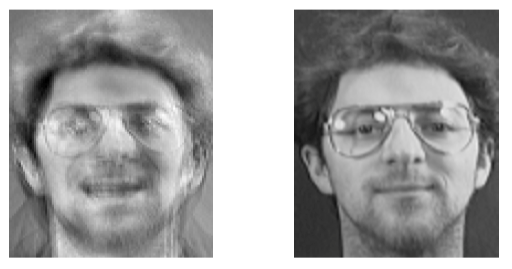
\includegraphics[width=0.7\linewidth]{chapter1_2.png}
  \caption{通过对机器学习模型获取的人脸信息(左)与一张模型训练图片(右)的对比\cite{Fredrikson2015}}
  \label{fig:chapter1_2}
\end{figure}
% 成员推断攻击是指利用机器学习模型的输出数据,最终判断某条记录是否被用于训练的攻击方法。这些篇\cite{7958568,10.1145/3243734.3243855,2018arXiv180601246S,8634878}均是关于成员推断攻击的工作。
% 三种方法相同点和不同点的对比如表~\ref{tab:model-attack-difference}所示。
% \begin{table}
%     \centering
%     \caption{机器学习模型攻击方法的对比}
%     \begin{tabular}{lll}
%       \toprule
%       攻击类型  & 攻击途径 & 攻击目标  \\
%       \midrule
%       模型抽取攻击   & 利用模型API输出 & 获取模型 \\
%       模型逆向攻击   & 利用模型API输出 & 获取统计信息                    \\
%       成员推断攻击 & 利用模型API输出  & 判断某记录是否被用于训练模型  \\
%       \bottomrule
%     \end{tabular}
%     \label{tab:model-attack-difference}
% \end{table}

% 随着越来越多针对机器学习模型攻击的产生,机器学习模型的信息泄露问题应当得到重视。一些用户不希望自己隐私数据被用来训练模型,因此一些已经训练好的模型想办法将这部分用户的数据进行“遗忘”。

\subsection{“被遗忘权”}
2018年5 月25日,欧盟正式施行《通用数据保护条例》(General Data
Protection Regulation)\cite{gdpr2018},简称GDPR。GDPR保护了一个人可能产生的任何数
据资料,包括个人身份,电话号码、地址、车牌等;生物特征,指纹、面部
识别信息、视网膜扫描信息等;电子记录,Cookie、IP位置、移动设备ID、
社交网络活动记录等。虽然GDPR是欧盟出台的一部条例,但其适用范围却很广\cite{visser2017,10.1007/978-3-030-21752-5_4,Kwak2017LetMU,Francesco2018}。
比如一家中国公司如果有来自欧盟国家的客户,这家公司也会受到GDPR的管辖。
GDPR在第三章第十七条中提出数据提供者拥有“被遗忘权”\cite{sarkar:hal-01824058,VILLARONGA2018304}。“被遗忘权”曾在
1995年就被欧盟提出,它是指数据提供者拥有让数据持有者删除其个人数据的
权利,包括数据的任何连接、副本和复制品。 “被遗忘权”不仅在欧盟出现,
在美国2020年1月1日正式施行的《加州消费者隐私法案》(The California
Consumer Privacy Act,简称CCPA)\cite{ccpa2020}中也提出了“被遗忘权”的概念(其概
念与GDPR基本类似,只有在例外情况的定义上有些许不同)。另外我国国家司
法部2019年5月28日颁布的《数据安全管理办法(征求意见稿)》\cite{gbt35273}中也明确
提出了用户有要求数据管理者删除其个人信息的权利。谷歌公司在2016年就曾
因为不符合欧盟的“被遗忘权”而收到了欧盟10万欧元的罚单,原因是谷歌并未按照用
户要求删除引用用户姓名的相关链接。



% 用户的被遗忘权早在2016年就被欧盟在《通用数据保护条例(GDPR)》提出。《通用数据保护条例(GDPR)》\cite{gdpr2018}(以下简称“GDPR”)是由欧盟2016年4月正式提出,并于2018年5月25日正式生效。
% GDPR的生效取代了欧盟自1995年实施的《数据保护指令》。与《数据保护指令》相比,GDPR更加注重隐私保护的实施细节,从而更好地保护用户的隐私数据。在GDPR的第三章第17条中提到了“Right To Be Forgotten”。
% 文章中写道,当用户撤销数据使用授权的时候,数据控制人应当立即删除用户数据以及其拷贝、连接和复制品。这就意味着如果一个公司从一个用户那里获取了一张用户提供的图片用于机器学习,那么当这个用户要求公司遗忘数据时,这个公司应当立即删除用户提供的图片,并且将机器学习模型恢复到没用这张图片学习的状态。
% 一旦这家公司真的这么做,就会面临一个挑战,那就是要重新训练机器学习模型,这样的代价是非常大的,因为机器学习的训练往往需要很长时间,几个小时、几天甚至几周。
% 此外,GDPR适用范围是很广的。在第3条适用范围中指出,即使这个公司不在欧盟范围内,只要这家公司向欧盟内公民提供了服务并且从欧盟公民那里获取了数据,GDPR法规也对这样的公司也是适用的。
% 关于机器学习模型遗忘的评论文章\cite{visser2017,10.1007/978-3-030-21752-5_4,Kwak2017LetMU,Francesco2018}有很多,可见隐私保护法规的力度开始逐渐显现。

% 关于隐私保护的法规不仅有GDPR,在2020年1月,美国《加州消费者隐私法案(California Consumer Privacy Act)》\cite{ccpa2020},简称“CCPA”,正式生效。
% 该法案的一个很大特点就是适用范围很广,这个法案的适用范围不仅包含注册或经营地址在加州的企业,也包含向加州居民提供服务或出售商品的企业和公司\cite{jiahui2020}。
% 和GDPR相同,CCPA也对用户的被遗忘权进行了保护,规定消费者有权利要求数据控制者删除从消费者收集的信息。

% 我国也有个人信息保护相关的国家标准\cite{gbt35273},这个标准中也指出个人信息主体有要求删除个人信息的权利。

% \subsection{当今卷积神经网络的主要应用}
% 卷积神经网络的一个应用是图像的分类和检索。图像的分类就是输入图片以后,输出这张图片在若干指定类别中最有可能的类别。图像分类常使用监督式的机器学习方法。
% 在使用卷积神经网络以前,常用的监督式机器学习有k近邻分类算法(K-nearest-neighbours,KNN),主成分分析法(Principle Component Analysis, PCA)以及支持向量机分类方法(Support Vector Machine, SVM)\cite{zhouzhihua2016}。
% 这些传统机器学习方法的一个共同点是需要提前提取特征。而卷积神经网络则不用,卷积操作会自动捕捉图像中的模式。特征的自动提取使得机器学习受到了广泛的欢迎,也使得卷积神经网络被科研工作者和企业工程师广泛接受。卷积神经网络因此也常常用作特征提取器。利用卷积神经网络进行图像分类的典型应用场景是图像搜索。
% 这个发明\cite{lingqiang2016}就提出了一种利用卷积神经网络进行快速图片检索的方法,并且把卷积神经网络当作特征提取器来使用,再结合其他基于特征距离的分类方法实现快速的图片检索。
% \begin{figure}
%   \centering
%   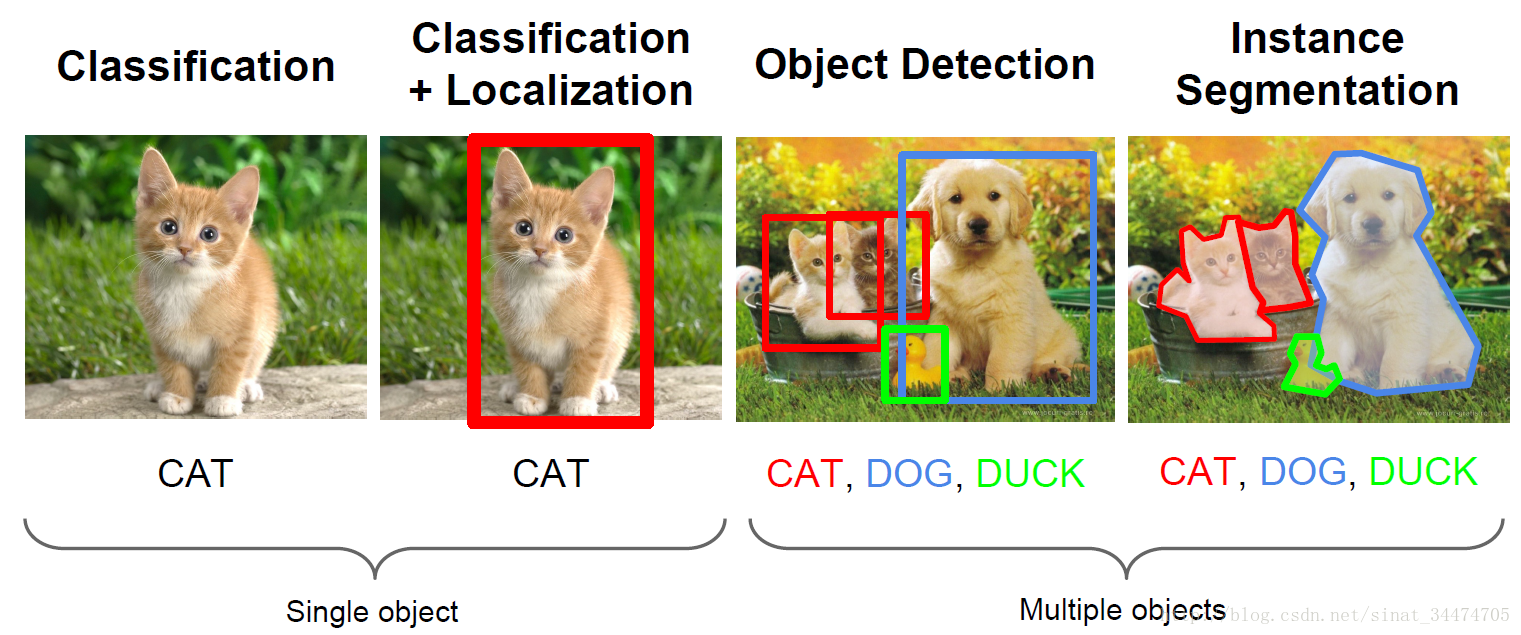
\includegraphics[width=0.9\linewidth]{chapter1_1.png}
%   \caption{图形分类、目标定位、目标检测和图像分割的不同\cite{mubiaodingwei}}
%   \label{fig:chapter1_1}
% \end{figure}

% 卷积神经网络另一个应用是目标的定位、检测和图像的分割。目标定位的任务是标出图片中物体的位置。目标定位和图像分类都有检测物体类别的属性,它们的不同点是目标定位除了要判别图片中有什么物体之外,还要给出物体在图片中的位置,一般用方框来标记物体位置。
% 目标检测的任务是识别图片中不定数量物体以及他们各自所在的位置。目标检测与目标定位的不同之处在于目标定位中物体的数量是固定的,而目标检测中物体的数量不是固定的。就是说目标检测需要把图片中所有目标物体全都识别出来并且准确地给出它们的位置。
% 图像分割的任务是在像素级别圈出图片中的目标物体。图像分割与目标检测不同的地方是图像分割是在像素级别将物体圈出,而目标检测则不需要这么精细,只需要用方框圈出大致的范围即可。如图\ref{fig:chapter1_1}所示,图中用图形展示了图形分类、目标定位、目标检测和图像分割的不同之处。
% 目标定位和目标检测的典型应用场景是自动驾驶、安全防护和医疗领域。图像分割常用于视频的后期制作和图像处理软件中,如Photoshop、美图秀秀等。

% 人脸识别技术被广泛应用在移动支付、门禁认证以及考试防作弊等场景。随着人脸识别技术的发展,人脸识别的底层技术也应用到了卷积神经网络。
% 人脸识别顾名思义就是在图像或视频中识别出人脸的技术。和图像分类技术类似,早期人脸识别技术采用的是传统机器学习的方法。其过程一般是通过摄像头获取图像或视频,然后通过计算机对图片或视频进行预处理,通过选取关键点来提取图片特征,再将提取出来的图片特征与训练好的模型进行比对,从而决定图片的分类。
% 这种方式虽然在一定程度上可以达到比较理想的效果,可是实际的图片情况是复杂的,比如图片中面部表情不同,光照角度不同,头部姿势不同和遮挡等情况经常出现,这就使得传统的人脸识别技术很难应对。
% 以卷积神经网络技术为代表的深度学习技术逐渐取代了传统人脸识别的方法,卷积神经网络可以通过学习大量的数据集而找到分类的本质特征,从而达到理想的分类效果。
% 2014年以DeepFace为代表的利用深度神经网络进行人脸识别的工作相继出现,使得人脸识别准确率不断提高。2015年FaceNet在LFW数据集上达到99.67$\%$的准确率,宣布人工智能首度超过人类的人脸识别能力。随着人脸识别技术的不断成熟,其应用场景也不断增多,如安全防护,金融认证,考试防作弊等,深入到我们日常生活的诸多方面。

% 卷积神经网络不仅用于图像的处理,其在自然语言处理方面也有出色表现。自然语言处理主要研究人类语言如何快速准确地被计算机系统识别和利用的技术。当今自然语言处理被广泛应用在语言翻译,文章主要观点的概括,语音的辨识等方面。
% 卷积神经网络由于其出色的特征提取和分类能力,如今也广泛被应用在自然语言处理领域中。

\subsection{选题意义和主要挑战}
从“被遗忘权”的概念联想到如今广泛使用的人脸识别模型,我们期望机器
学习具有遗忘掉数据的功能,就好像这些数据从来没有被训练过一样。当前的机
器学习算法大部分只有正向学习的部分,而如何让模型遗忘掉一些训练数据却缺
乏一些通用的方法。因此,研究如何让机器学习模型拥有遗忘能力具有十分重要
的现实意义。本课题正是基于这一方向出发,面对人脸识别的应用场景,探索卷积神经网络的高效率数据遗忘方法。

目前,主流的人脸识别模型大多基于卷积神经网络\cite{GUO2019102805}。比如Facebook的
DeepFace模型\cite{deepface2014},将人脸识别能力提高到与人类相媲美的水平。
卷积神经网络现在仍然是一个“黑箱子”,把数据按照一定的方法进行训练,就能得到效果很好的分类模型。可是我们仍然不清楚网络中每个参数代表的具体意义。
还有,解决机器学习模型遗忘问题的一个朴素方法是完全重新训练模型。这样的方法需要付出很多成本。
再有,遗忘方法好坏的另一个考虑因素是该方法能否被重复使用。因此遗忘的可持续性也是一个很大的挑战。

% 当今的神经网
% 络结构越来越复杂,种类也多种多样。DeepFace模型的结构包含
% 5个卷积层、1个池化层和2个全连接层。
% 在众多的神经网络结构中找到一种通
% 用有效的遗忘方法是十分困难的。面对越来越庞大且复杂的神经网络模型,如何
% 提高数据遗忘的速度也是巨大的挑战。
% \begin{figure}
%   \centering
%   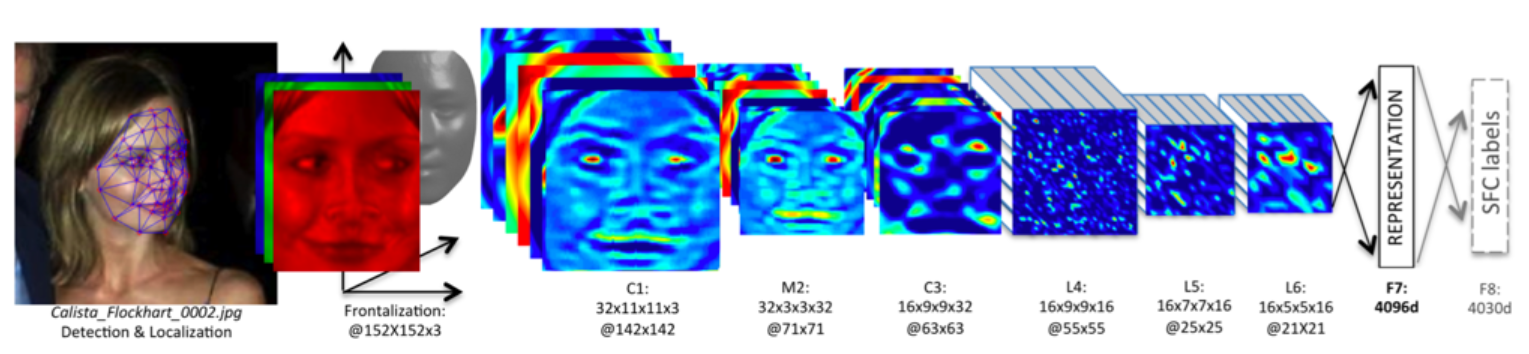
\includegraphics[width=0.9\linewidth]{chapter1_3.png}
%   \caption{DeepFace模型结构\cite{deepface2014}}
%   \label{fig:chapter1_3}
% \end{figure}

% 随着卷积神经网络的广泛应用,越来越多的机器学习模型选择卷积神经网络进行学习。与此同时,对机器学习模型的攻击也是层出不穷,用户个人隐私保障的问题急需解决。
% 随着GDPR的正式施行,用户个人数据的被遗忘权也得到了法律的保护。目前可行的方法是将模型重新训练,可是这样的做法会给企业带来很大的经济负担。
% 于是研究如何加快基于卷积神经网络的机器学习模型遗忘的算法势在必行。据作者目前了解的情况来看,尚未有一个很成熟的可以大规模使用的基于卷积神经网络的机器学习遗忘算法。
% 因此,在人们的隐私意识逐步提高的今天,研究基于卷积神经网络的机器学习遗忘算法具有十分重要的现实意义。

% 机器学习模型遗忘方面的研究从2015年逐渐有学者开始发表论文。刚开始的研究方向是基于一些经典的机器学习算法,比如文献\cite{yinzhicao2015}尝试解决基于贝叶斯推断的遗忘方法,文献\cite{antonio2019}基于k-means聚类算法的遗忘方法等等。
% 逐渐地,随着欧盟GDPR法规的出台,开始有学者把视线转移到了研究卷积神经网络的遗忘。目前基于卷积神经网络的遗忘仍然是一个开放的问题,尚且没有统一的办法来解决这个问题。

% 近年来尝试解决卷积神经网络遗忘问题的方法多种多样,例如一种基于网络分割的方法\cite{2019arXiv191203817B},通过将网络分割成若干个小网络,使得重新训练的任务量从整个大网络减小成每个小网络重新训练的工作量。
% 这样的方法虽然在重新训练时间上面有所降低,同时也带来需要将所有网络预测结果进行综合的额外工作量,使得网络在进行预测时效率有所降低。
% 还有一种思路是基于正则化和增加噪音的方法,这个方法\cite{Golatkar_2020_CVPR}通过重新设计损失函数并且在权重上增加随机噪音的方法实现遗忘效果。
% 这种方法能达到很迅速遗忘的效果,可是增加噪声会不可避免地减少没被遗忘类别的准确率。总之到目前为止,尚没有一种方法取得了压倒性的优势,因此基于卷积神经网络的遗忘问题仍然是开放的。

% 基于卷积神经网络的遗忘问题之所以这么困难是因为卷积神经网络的非线性特征,这种非线性特征使得人们很难寻找其参数更新的规律,换句话说就是可解释性很差。在输入多个训练数据参与训练之后,我们无法通过反向还原的方法通过数学计算将网络还原到训练之前的那个状态。
% 虽然卷积神经网络的优点有很多,可是卷积神经网络现在对人类来说仍然是一个黑箱,无法寻找到卷积神经网络参数更新的规律。因此,寻找如何更新参数的方法就是本研究方向的一个挑战。

% 另外,卷积神经网络模型利用遗忘算法遗忘过后,如何评价遗忘的效果也是这个研究方向的一个挑战。我们的一个直觉是通过测试的准确率来评价遗忘效果。经过分析后发现,这个指标仅能作为一个辅助指标进行参考。
% 因为遗忘问题的本质并不是遗忘得越彻底越好,如果通过掩盖的方法来降低遗忘类别的准确率反而能够给攻击者可乘之机。因为攻击者可以利用成员推断攻击来判断一个训练数据是否曾经被用于网络模型的训练,这种情况往往也不是用户期待发生的事情。这种情况可以被一个词很好的描述,“欲盖弥彰”。
% 因此,如何评价网络模型已经达到了一个理想的遗忘效果也是本文的一个挑战。

\section{主要研究方法}
为了解决卷积神经网络的遗忘问题,本文利用了卷积神经网络的一个重要特性,分层抽象特性。在卷积神经网络中,一个个卷积核就是特征的提取器,在不同的网络层次中,这些提取器对特征提取的分工是各不相同的。
较低层次的特征提取器会提取一些基本特征,随着网络层次的提高,特征提取器会提取一些较为抽象的特征。我们利用了这一特性,提出了一种更新网络参数的策略,只更新和最终分类相关的较高层次的网络参数,随后再利用保留集训练网络,直至网络收敛。
实验结果表明,这种方法在不用更新全部网络参数的情况下能够达到理想的遗忘效果,而且遗忘时间也较完全重新训练快一倍以上。本文的贡献可以分为以下几个方面:

第一,本文提出了一种更新网络参数的方法。经实验证明这种方法可以达到很好的遗忘效果,而且在遗忘时间方面比完全重新训练要快。

第二,经过实验表明,本文提出的方法具有遗忘的连续性,适用于多次遗忘操作,本文方法具有一定的应用前景。

第三,本文通过反向冻结实验验证了卷积神经网络的分层抽象特性并且验证冻结网络部分参数可以提高网络收敛速度。

\section{论文结构安排}
第一章是引言,首先介绍了本文的研究背景和选题意义;然后简要说明了本文中所用到的解决问题的思路和方法;最后提出了本文的主要贡献。

第二章首先介绍了机器学习遗忘的研究工作,包括非神经网络的遗忘方法和神经网络的遗忘方法;然后介绍了基于参数共享思路的机器学习方法,主要讲了迁移学习和增量学习的相关研究领域。

第三章是本文的核心章节,首先介绍了卷积神经网络的基本原理与本文解决遗忘问题的思路来源,即分层抽象特性;然后分步骤具体介绍了遗忘问题的解决方案;最后介绍了评价遗忘效果的三个指标。

第四章是实验验证,首先介绍了本文实验所用到的实验环境;然后介绍了三个实验方法的实现方式;最后结合图片对实验结果的进行了展示。

第五章是全文的总结,首先总结了各个章节的主要内容;然后讲了本文的不足之处;最后对基于卷积神经网络遗忘方法可能的发展方向进行了展望。

% !TeX root = ../thuthesis-example.tex

\chapter{相关工作}

本章第一节中首先介绍关于机器学习模型遗忘方法的研究。这一节中将重点介绍基于神经网络遗忘方法的相关工作。为了解决基于卷积神经网络的遗忘问题,本文借鉴了关于神经网络相关研究领域的一些解决问题的方法,比如共享参数的网络微调的方法。
一些研究领域通过使用此方法可以达到减少训练工作量,使模型可持续使用的效果,如迁移学习和增量学习。关于这些领域的相关研究成果将在本章第二节中具体介绍。

\section{机器学习模型遗忘方法研究}
\subsection{非神经网络遗忘方法}
Yinzhi Cao\cite{yinzhicao2015}最早引入了机器学习遗忘的研究,该工作使用了统计查询学习\cite{10.1145/293347.293351}的方法对基于贝叶斯方法的机器学习进行了遗忘算法的设计。
基于贝叶斯模型的遗忘方法还有文献\cite{10.1145/3196494.3196517}。
Antonio Ginart等人\cite{antonio2019}对于k-means机器学习的方法设计了遗忘某一个类别的算法。
Anthony D’Amato\cite{10.1007/978-3-319-40159-1_19}提出了一种基于决策树的遗忘算法。本文将讨论基于卷积神经网络的遗忘方法,暂不对非神经网络的遗忘方法进行讨论。

\subsection{基于神经网络遗忘方法}
Bourtoule Lucas等人\cite{2019arXiv191203817B}提出了一种可以用在神经网络上的遗忘方法,过程如图\ref{fig:machine_unlearning}所示。
作者首先将训练数据集分成若干互不相交的部分,然后利用每个部分单独训练出一个神经网络模型。网络最终输出的结果将多个神经网络模型输出的结果综合起来,最终输出一个结果。
遗忘的时候,只需要重新训练要遗忘的训练样例所在的神经网络,而无需重新训练所有神经网络模型。这样的方式虽然能够减少重新训练的工作量,但仍未摆脱重新训练的模式,而且训练如此多的神经网络也造成了参数的浪费。
\begin{figure}
    \centering
    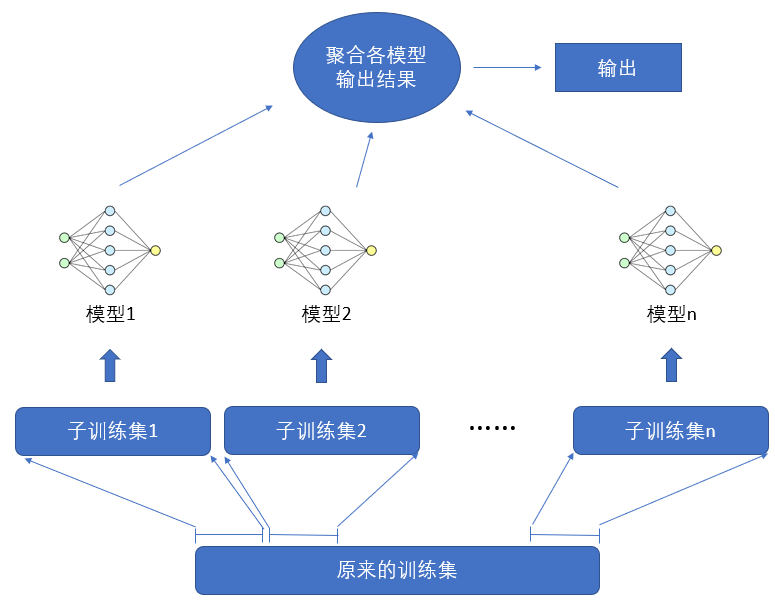
\includegraphics[width=0.7\linewidth]{machine_unlearning.png}
    \caption{将数据集分成若干互不相交集合分别训练}
    \label{fig:machine_unlearning}
\end{figure}
% \begin{figure}
%     \centering
%     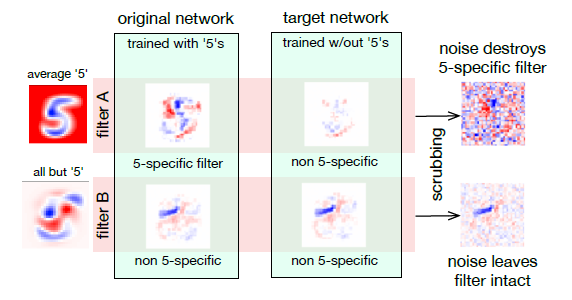
\includegraphics[width=0.9\linewidth]{eternal_sunshine.png}
%     \caption{基于增加噪音和正则化的遗忘方法\cite{2019arXiv191203817B}}
%     \label{fig:eternal_sunshine}
% \end{figure}

Golatkar Aditya等人\cite{Golatkar_2020_CVPR}实现了一种通过在权重上增加噪音的方法来逐渐减少神经网络参数对遗忘数据的信息量
% ,如图~\ref{fig:eternal_sunshine}所示
。这篇文献提出了一些值得借鉴的衡量遗忘效果的指标,比如遗忘集的测试准确率,保留集的测试准确率。
文献中还提出了模型置信指标,计算目标神经网络与此文方法遗忘之后的网络在遗忘集和保留集上的交叉熵。这些指标在实际应用上具有参考价值,因此本文也引用了这些评价指标。
文献中还提到了一种信息论领域常用到的信息边界衡量方法,计算两个网络模型参数的KL散度距离(Kullback-Leibler Divergence),这种方法经常用于量化两个随机变量概率分布的相似性。
然而,遗忘的目的并不只是简单地让网络的参数去接近目标网络,而是在实际效果上看两个网络的输出是否相近。因为思路上有本质的不同,所以这个衡量指标并没有被本文所采用。这个方法虽然在遗忘的效果上达到了较为理想的状态,然而保留类别的准确率并不是很理想。

Aditya Golatkar等人\cite{Golatkar_2021_CVPR}提出了一种混合训练模型,将训练集分为核心训练集和用户训练集。核心训练集表示学习后不会被遗忘的训练集,用户训练集代表学习后可能会被用户遗忘的训练集。文章中使用了两个神经网络用来训练。
在遗忘时,只去更新使用用户集训练的网络,而使用核心数据集的网络保持不动。该工作通过正则化加噪音的方法实现了遗忘算法,使用的遗忘指标是遗忘集、保留集和测试集的准确率、重新学习时间、激活距离还有成员推断攻击的成功率。
本文引用了其中的激活距离这个指标用于评价遗忘方法的效果,以测量两个网络的输出差异。

关于神经网络遗忘算法的相关工作仍有很多种思路,如Golatkar Aditya\cite{10.1007/978-3-030-58526-6_23}和Guo Chuan\cite{pmlr-v119-guo20c}等人使用牛顿更新的方法。
Izzo Zachary等人\cite{pmlr-v130-izzo21a}使用了基于影响函数\cite{pmlr-v70-koh17a,cook_weisberg_1982}的思路。
Wu Yinjun等人\cite{pmlr-v119-wu20b}利用训练过程中存储的数据进行了参数还原。
Neel Seth等人\cite{pmlr-v132-neel21a}通过增加噪声实现遗忘。
Du Min等人\cite{10.1145/3319535.3363226}利用了反向更新梯度的方法实现异常检测模型的还原。
相关工作的比较情况如表\ref{tab:forget-methods}所示,我们从遗忘方法是否修改了网络参数,是否修改了损失函数,是否使用了保留集训练等七个方面进行了对比。
通过比较可以看出,大部分的方法都使用了修改网络参数的办法而且遗忘时需要使用保留集进行训练。另外,仅有本文考虑到了卷积神经网络的分层抽象特性。

\begin{table}
    \centering
    \caption{神经网络遗忘方法相关工作比较}
    \begin{tabular}{p{3cm}<{\centering}p{1cm}<{\centering}p{1cm}<{\centering}p{1cm}<{\centering}p{1.5cm}<{\centering}p{1.5cm}<{\centering}p{2cm}<{\centering}}
    %\begin{tabular}{ccccccc}
      \toprule
      相关论文  & 修改网络参数 & 修改损失函数  &修改网络结构&遗忘时使用遗忘集训练&遗忘时使用保留集训练&考虑了卷积神经网络的分层抽象特性\\
      \midrule

      Aditya Golatkar et al.\cite{Golatkar_2020_CVPR} &\checkmark&\XSolidBrush&\XSolidBrush&\XSolidBrush&\checkmark&\XSolidBrush \\
      Aditya Golatkar et al.\cite{Golatkar_2021_CVPR} &\checkmark&\checkmark&\XSolidBrush&\XSolidBrush&\checkmark&\XSolidBrush \\
      Aditya Golatkar et al.\cite{10.1007/978-3-030-58526-6_23} &\checkmark&\XSolidBrush&\XSolidBrush&\XSolidBrush&\XSolidBrush&\XSolidBrush \\
      Baumhauer Thomas et al.\cite{2020arXiv200202730B} &\XSolidBrush&\XSolidBrush&\checkmark&\checkmark&\XSolidBrush&\XSolidBrush \\
      Bourtoule Lucas et al.\cite{2019arXiv191203817B} &\checkmark&\XSolidBrush&\checkmark&\XSolidBrush&\checkmark&\XSolidBrush \\
      Guo Chuan et al.\cite{pmlr-v119-guo20c} &\checkmark&\checkmark&\XSolidBrush&\XSolidBrush&\checkmark&\XSolidBrush \\
      Izzo Zachary et al.\cite{pmlr-v130-izzo21a} &\checkmark&\checkmark&\XSolidBrush&\XSolidBrush&\checkmark&\XSolidBrush \\
      Wu Yinjun et al.\cite{pmlr-v119-wu20b} &\checkmark&\XSolidBrush&\XSolidBrush&\checkmark&\XSolidBrush&\XSolidBrush \\
      Neel Seth et al.\cite{pmlr-v132-neel21a}方法一 &\checkmark&\XSolidBrush&\XSolidBrush&\XSolidBrush&\checkmark&\XSolidBrush \\
      Neel Seth et al.\cite{pmlr-v132-neel21a}方法二 &\checkmark&\XSolidBrush&\checkmark&\XSolidBrush&\checkmark&\XSolidBrush \\
      本文 &\checkmark&\XSolidBrush&\XSolidBrush&\XSolidBrush&\checkmark&\checkmark \\

      \bottomrule
    \end{tabular}
    \label{tab:forget-methods}
\end{table}

\section{可共享网络参数人工神经网络相关研究}

\subsection{迁移学习相关研究}
该工作\cite{10.1007/978-3-030-01424-7_27}给迁移学习下的定义是给定一个数据集$D_t$和一个学习任务$T_t$,这个学习任务可以从另外一个基于数据集$D_s$的学习任务$T_s$获得帮助,从而加快学习任务$T_t$的学习进程。
这个概念中要解决的问题和我们面临的遗忘问题如出一辙。文中将迁移学习分为四类,即基于对抗的迁移学习,基于网络的迁移学习,基于映射的迁移学习以及基于实例的迁移学习。
其中基于网络的迁移学习提出了共享网络参数来加快目标网络的学习,将一个神经网络的前若干层结构和参数迁移至另一个新的神经网络,将这些网络连接和学习参数作为新的神经网络的一部分。
Jui-Ting Huang等人\cite{6639081}也采用了类似的思路,实现了语言识别的功能。作者将网络分成两个部分,前一部分是语言独立的特征提取器,最后一层是语言相关的分类器。
神经网络的输入是不同语言的语音片段,经过共享的特征提取器,输出到最后的全连接层。最后全连接层实现语言分类的功能。文中指出,对于使用欧洲的四种语言训练出来的网络,与使用单个语言训练的网络相比,单词的错误率下降了3\%-5\%,证明了共享网络参数方法的有效性。
Oquab Maxime等人\cite{Oquab_2014_CVPR}讲到了共享特征的方法。网络可以分成两个部分,一部分是卷积层,另一部分是全连接层。
先将网络在一个训练集上训练,训练完成后,将卷积层和若干全连接层迁移到另外一个分类任务当中,替代网络中的卷积层和若干全连接层。
为了更好地适应新的分类任务,新增了两层全连接层,然后使用新的训练集对网络进行训练,训练的同时冻结迁移过来的参数,只训练新增的全连接层参数。训练至收敛后,网络同样取得了很好的效果。 

Yosinski Jason等人\cite{yosinski_2014_NIPS}对深度神经网络特征可共享的特性进行了研究。如图\ref{fig:transfer_learning_3}所示,第一行代表用数据集1训练的网络,第二行代表用数据集2训练的网络。
第三行代表将前三层参数进行训练,其中实验将冻结参数和不冻结参数训练分开进行。在训练之前,先将第二行前三层的参数迁移至第三行前三层参数。第四行代表前三层参数使用第一行训练好的前三层参数,之后将这三层参数进行训练,冻结参数和不冻结参数训练也是分开进行。
冻结参数是将网络参数只用于网络的预测,在网络训练过程中不进行更新。
最终的结果是使用不冻结参数方法的一组,并且使用不同数据集训练的网络得到了很好的泛化效果。从这个实验中可以看出,深度神经网络前若干层参数是可以共享的。
\begin{figure}
    \centering
    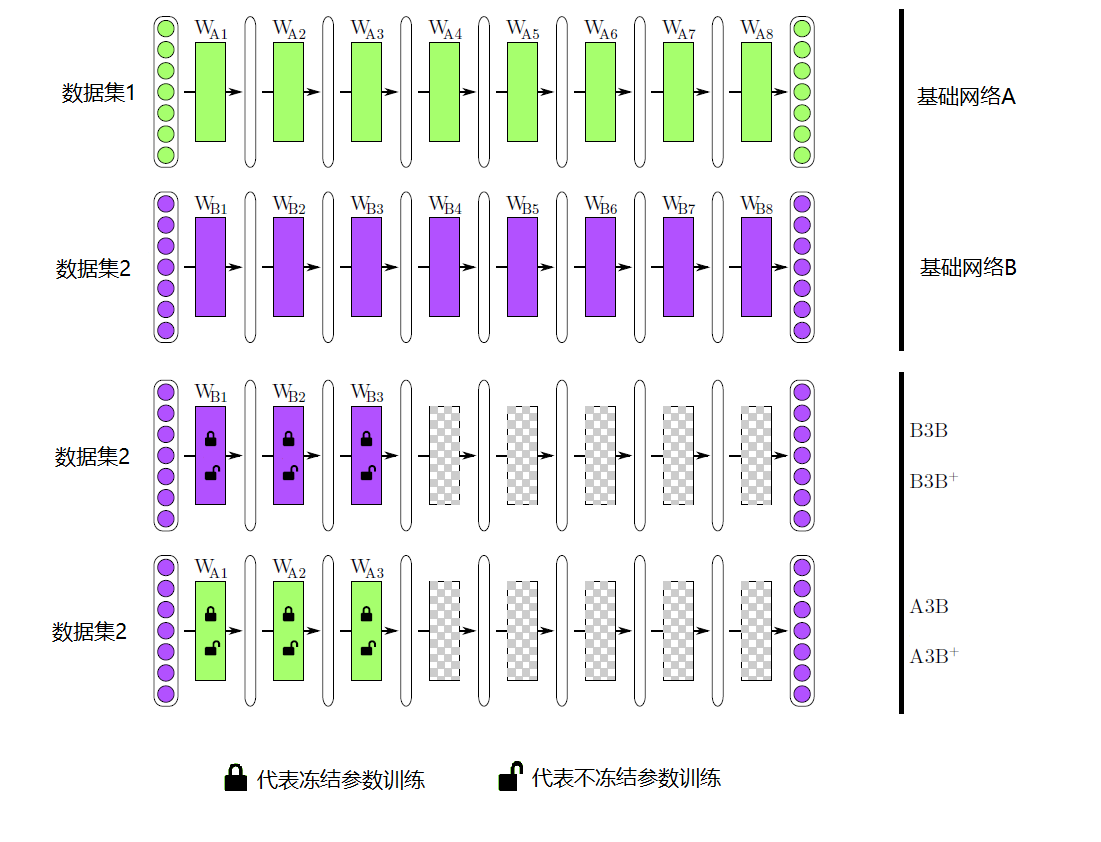
\includegraphics[width=0.9\linewidth]{transfer_learning_3.png}
    \caption{共享参数的深度神经网络训练示意图}
    \label{fig:transfer_learning_3}
\end{figure}

\subsection{增量学习相关研究}
增量学习是指在已经学习完成的机器学习模型上继续学习新数据的方法。增量学习面临的困难是灾难性遗忘,即在已经学习完成的机器学习模型上只用新的数据集去训练会出现旧的分类测试准确率出现下降的情况。
为了克服灾难性遗忘,German Parisi等人\cite{PARISI201954}提到了增量学习大致可分为三种类型:基于正则化的方法,基于动态结构的方法以及基于补充学习系统和记忆重放的方法。其中,基于动态结构的方法使用了共享网络参数的方法。

Zhizhong Li等人\cite{8107520}对增量学习的方法进行了分类。如图\ref{fig:incremental_learning_1}所示,图中展示了一个已经学习完成的网络在遇到新的学习任务时可能的学习方法。
(a)中是原来已经学习好的模型,前半部分是卷积神经网络,后半部分是全连接层。当加入一个新的类别后,大概有三种可能的解决方法。
子图(b)一种是微调训练(Fine-tuning),即在原来的网络上用新的训练数据直接训练。这样的方法会导致灾难性遗忘。
子图(c)是特征提取(Feature Extraction),和以前训练好的网络分享一部分参数,将这部分参数冻结,然后用新的训练数据继续训练没有被冻结的参数。
子图(d)是联合训练(Joint Training),用新的训练数据和旧的训练数据同时训练原有的网络。这样带来的效果是比较好的,但是重新训练的成本很大。
这样的方法可能的问题是新的训练数据也具有自己独特的数据特征,这样的特征由于网络参数的冻结而无法被原有网络提取,因此最终的效果也不会很好。
\begin{figure}
    \centering
    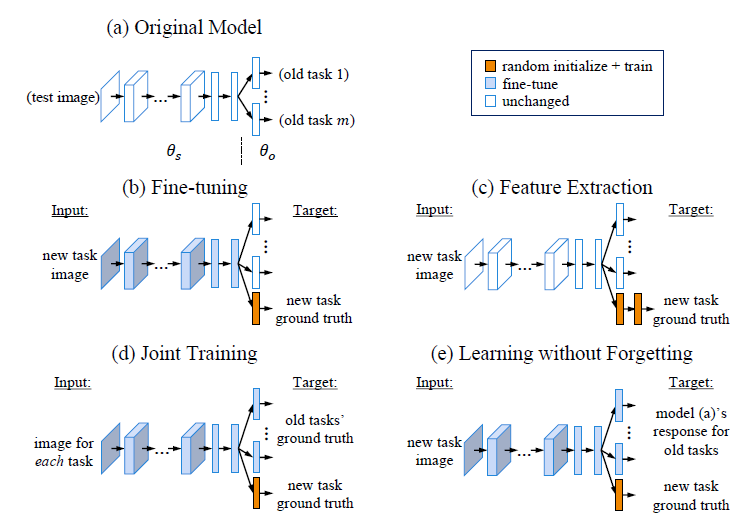
\includegraphics[width=0.9\linewidth]{incremental_learning_1.png}
    \caption{增量学习方法分类}
    \label{fig:incremental_learning_1}
\end{figure}

Sarwar Syed Shakib等人\cite{Sarwar_2020}通过共享网络层次,建立新网络分支来解决灾难性遗忘的问题。如图\ref{fig:incremental_learning_2}所示,原来的网络已经训练了50个类别,当有10个新的类别需要添加到网络中时,首先确定好共享网络的层次,然后冻结共享网络和原来分类网络的参数,最后只用新的训练数据对新增加的网络进行训练。
当需要做预测时,将两个网络的输出综合起来,判断应当输出的结果。这样的网络随着新类别的增加而逐渐变得庞大。但是我们从中可以借鉴到共享网络参数的思想。
\begin{figure}
    \centering
    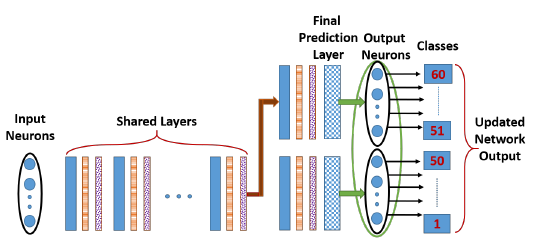
\includegraphics[width=0.7\linewidth]{incremental_learning_2.png}
    \caption{共享网络参数的增量学习}
    \label{fig:incremental_learning_2}
\end{figure}


\section{本章小结}
本章首先介绍了机器学习模型遗忘方法的相关研究工作情况,包括神经网络无关的机器学习模型的遗忘方法和一些基于神经网络的遗忘方法。虽然基于卷积神经网络的遗忘还没有一套成熟的解决方案,但是这些相关工作具有重要的参考价值。
然后介绍了关于网络参数共享方面的人工神经网络的相关研究,主要列举了基于网络的迁移学习方向的相关工作和关于网络参数共享的增量学习方面的相关工作。
% !TeX root = ../thuthesis-example.tex

\chapter{卷积神经网络分层抽象特性和遗忘方法}
上一章阐述了遗忘学习的研究现状以及相关研究工作。本章首先介绍卷积神经网络的一个重要特性,分层抽象特性。为了让读者能够更好地理解卷积神经网络的分层抽象特性,首先将介绍卷积神经网络的工作原理以及设计思想。
接下来介绍卷积神经网络分层抽象特性和遗忘方法。最后介绍评价遗忘效果的性能指标。

\section{卷积神经网络介绍}

\subsection{卷积神经网络结构}
卷积神经网络和多层感知机的神经网络类似,它们都可以通过像堆积木一样来组装构建。卷积神经网络和多层感知机不同的是卷积网络特有的卷积层(Convolution Layer)和池化层(Pooling Layer)。

% 基于多层感知机的神经网络中,相邻层的各个神经元之间都有连接,这样的结构被称为全连接(Fully-Connected)。
% 如果使用全连接层来搭建网络,我们可以通过如图\ref{fig:chapter3_3}所示的神经网络结构实现一个五层的简单神经网络。
% 如图\ref{fig:chapter3_3}所示,在使用全连接层搭建的神经网络中,全连接层后面直接跟着激活函数ReLU(或者Sigmoid)。这里使用了4 层全连接和ReLU的组合,接着的第5层是全连接层,最后一层则是Softmax层,输出最终的预测结果。
% \begin{figure}
%     \centering
%     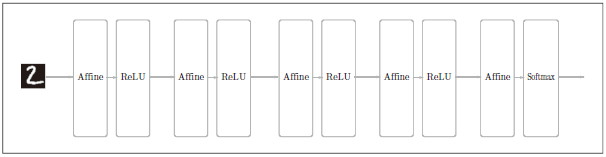
\includegraphics[width=0.9\linewidth]{chapter3_3.png}
%     \caption{全连接网络结构示意图\cite{luyujie_216}}
%     \label{fig:chapter3_3}
% \end{figure}
\begin{figure}
    \centering
    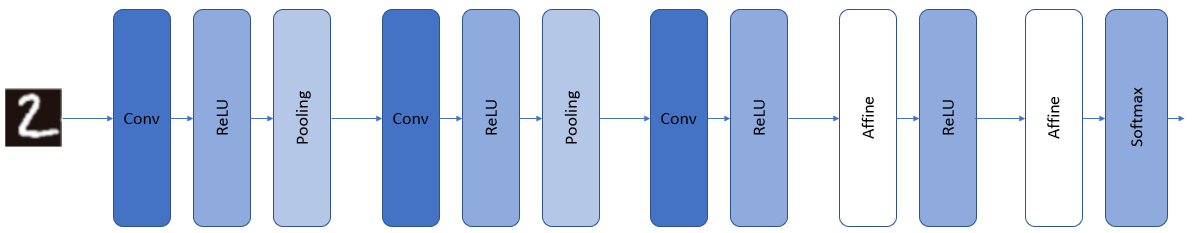
\includegraphics[width=0.9\linewidth]{chapter3_2.png}
    \caption{卷积神经网络结构示意图}
    \label{fig:chapter3_2}
\end{figure}

如图\ref{fig:chapter3_2}所示,这是一个卷积神经网络的例子。卷积神经网络的单个层连接的顺序是卷积层、激活函数层(如图中的ReLU层)和池化层,其中池化层有时可以省略。
然后,最终的输出层中则使用了全连接层和Softmax的组合。图中的Affine层代表全连接层。这样的搭配一般都是卷积神经网络中较为常见的搭配结构。
卷积层主要用来提取特征,激活函数层主要用来过滤卷积层提取到的特征,对输入的特征增加非线性的因素,因为线性模型的表达能力是有限的。池化层主要用来压缩数据和参数的量,因此也常被称为下采样层。
全连接层能够实现特征的空间映射,常被用来做分类器。Softmax层是对整个网络输出结果的优化表示,将神经网络的输出转换成概率分布的输出,以便于对网络输出的理解。

\subsection{卷积神经网络原理} 
\subsubsection{卷积神经网络对于位置关系的理解}
在全连接的神经网络中,每一层都是通过全连接层组织起来的。在全连接的层次中,各个神经元都是连接在一起的,其输出数量是可以任意指定的,没有数量上的限制。

这样的结构没有将数据的形状特征充分利用起来。用图片来举例,神经网络输入图片时,图片数据的格式一般是长、宽和高。长和宽代表图片以像素为单位的长度和宽度,高代表图片采样通道的宽度。
然而,这样的数据结构输入到全连接层搭建的神经网络中时,就会被展开成一维的数据。图片一般是三维的形状,即图片的长度和宽度,还有色彩的维度(红色通道,绿色通道,蓝色通道),这样的形状结构中包含了重要的空间位置关系信息。
比如色彩通道之间的关联信息,空间上相互距离比较接近的像素点一般具有相似的值,距离比较远的像素点一般没有关联。因此三维形状的数据中可能会蕴藏很多可以挖掘的特征模式。全是全连接层的神经网络就会把数据展开成一维数据,从而没有充分利用图片中的空间位置信息。
卷积神经网络会将图片以三维数据的格式输入到网络中,一个卷积层处理好数据以后,仍然会以三维的数据格式输入到下一个卷积层中。所以,卷积神经网络对于理解带有空间位置信息的数据具有一定的优势。

\subsubsection{卷积层}
卷积运算发生在卷积层,卷积运算的计算过程类似滤波处理的过程。因此用于卷积运算的卷积核有时又被称为滤波器。常规的卷积运算如图\ref{fig:chapter3_4}所示。
图中展示了一次二维卷积运算的运算过程。输入数据的尺寸是4乘4,卷积核的尺寸是3乘3,在没有边界填充并且步长为1的情况下,最终输出结果的尺寸是2乘2。
\begin{figure}
    \centering
    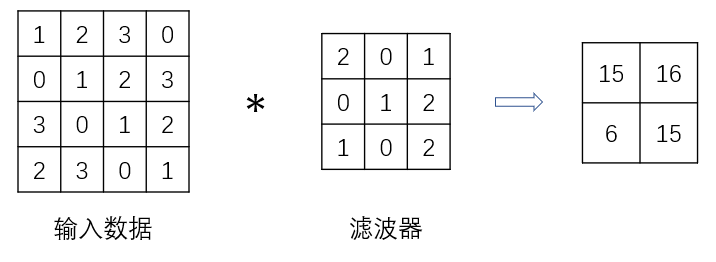
\includegraphics[width=0.6\linewidth]{chapter3_4.png}
    \caption{卷积运算后数据大小发生变化}
    \label{fig:chapter3_4}
\end{figure}

图\ref{fig:chapter3_5}中介绍了卷积运算的完整过程。图中第一行灰色区域代表第一步卷积操作所发生的区域,这个区域内的数字和卷积核的形状是相同的,所以区域内的数字可以与卷积核中对应位置的数字相乘,然后再把这些相乘的结果相加就得到了第一个结果。
运算后将结果保存到相应的位置。在图\ref{fig:chapter3_5}中第二、三、四行将上述过程在每个位置计算一遍,就完成了输入数据在一个卷积核上的特征输出。
\begin{figure}
    \centering
    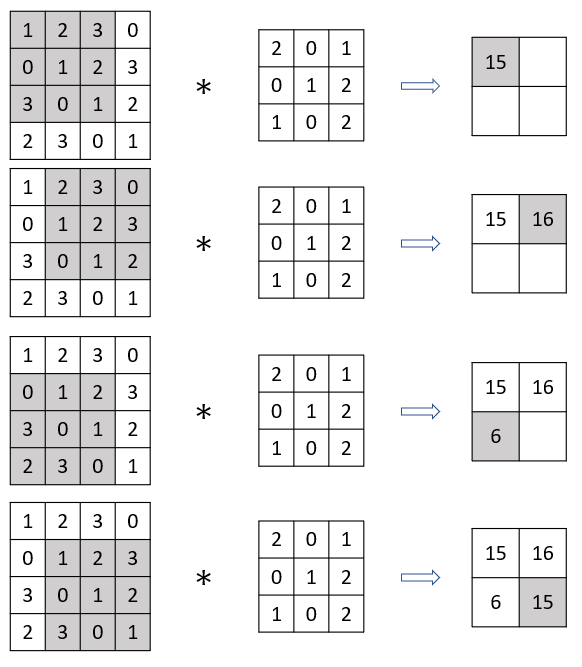
\includegraphics[width=0.5\linewidth]{chapter3_5.png}
    \caption{卷积运算过程示意图}
    \label{fig:chapter3_5}
\end{figure}

卷积神经网络中除了权重之外,还有偏置。卷积神经网络中偏置的个数一般就是卷积核的个数,而且每个卷积核对应的偏置维度一般是1乘1。
计算完卷积之后,在相应结果的每个位置再加上偏置数字便得到了最终输出的数据,其计算过程如图\ref{fig:chapter3_6}所示。
对于输入数据,滤波器与输入数据进行卷积运算后便得到了初步的输出结果。之后再将这个结果的每一个位置加上该卷积核对应的偏置数值,得到了最终结果。
\begin{figure}
    \centering
    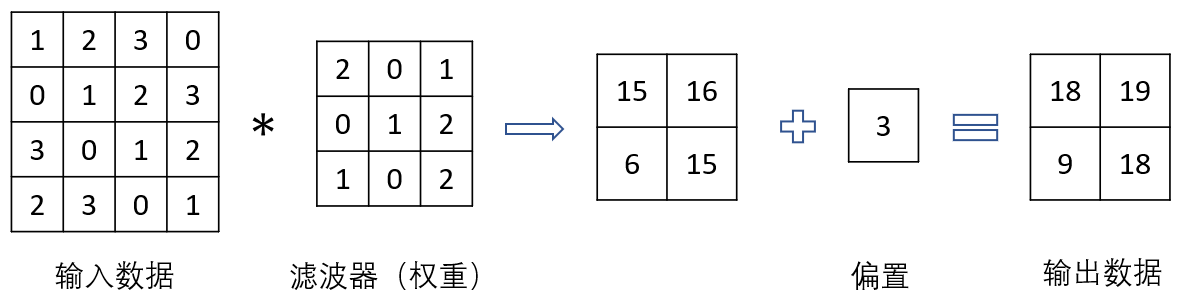
\includegraphics[width=0.7\linewidth]{chapter3_6.png}
    \caption{卷积运算后的偏置}
    \label{fig:chapter3_6}
\end{figure}

三维卷积运算与二维卷积运算不同的是,卷积核的维度从二维提高到了三维,除了有长和宽的信息,还有通道的维度。以三通道为例,其运算过程与二维相似,先将对应位置的数字相乘,然后将相乘之后的结果相加,便得到了输出结果。

\subsubsection{池化层}
为了减少参数的数量,提高神经网络泛化能力,在卷积神经网络进行卷积运算以后,通常会进行池化操作。池化操作会同时减少卷积操作结果的长度和宽度。
其运算过程如图\ref{fig:chapter3_8}所示。在图中第一行,灰色区域就是池化的一个操作单元。这个操作单元的大小来自池化操作的输入参数。
池化操作的输入是图中灰色区域内的数字,输出是一个数字。中间的运算过程一般有两个算法,一种是取所有数字中最大的数字,这种算法被称为最大池化操作;另外一种算法是取区域内所有数字的平均数,这种算法被称为平均池化操作。
\begin{figure}
    \centering
    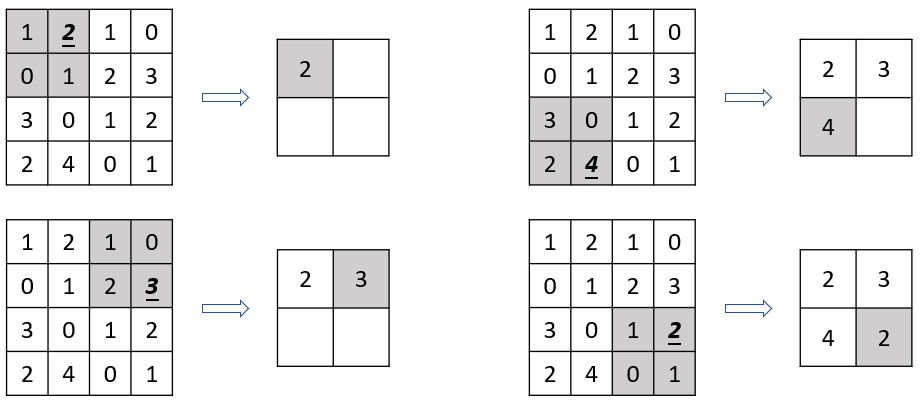
\includegraphics[width=0.7\linewidth]{chapter3_8.png}
    \caption{池化操作流程图}
    \label{fig:chapter3_8}
\end{figure}

池化层与卷积层不一样的是,池化层没有训练参数,它的输入参数都是运算之前系统已经规定好的超参数。池化层就是一个固定算法的函数。它另外的一个特点是,池化操作后通道数是不变的,各通道是相互独立的。
加入池化层后,神经网络对输入数据存在的微小干扰具有很好的鲁棒性。如图\ref{fig:chapter3_10}所示,即使图片向右发生了1个偏移,经过池化操作后,其特征仍能被准确地识别出来。
\begin{figure}
    \centering
    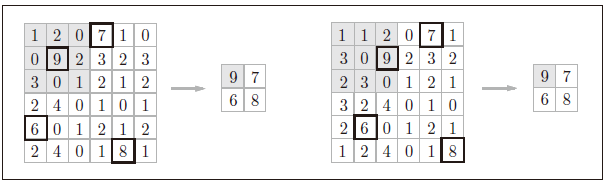
\includegraphics[width=0.9\linewidth]{chapter3_10.png}
    \caption{池化操作对发生偏移的输入具有鲁棒性}
    \label{fig:chapter3_10}
\end{figure}

\section{卷积神经网络分层抽象特性}
为了更好地理解卷积神经网络的分层抽象特性,我们首先简要地介绍生物视觉信息处理的原理。
\subsection{生物视觉系统对信息的分层处理}
1981年来自美国的科学家David Hunter Hubel和来自瑞典的科学家Torsten Wiesel被授予了诺贝尔生理学或医学奖,以表彰他们在探究人类视觉系统信息加工过程中做出的杰出贡献\cite{Hubel1998EarlyEO}。他们的工作成为了所有研究神经生物学学生们的必学内容。
他们使用探针记录了麻醉后猫的大脑视觉皮层神经元的活动\cite{https://doi.org/10.1113/jphysiol.1959.sp006308}。
他们在实验中发现,有一类细胞对一定视野范围内特定朝向上移动的狭长光斑反应强烈,而且反应的产生有明显的边界。方向不对或者超越边界都无法使之产生反应。
当光斑覆盖整个作用区域时,也无法产生刺激反应。这样的细胞被看作是用来感受线条或边缘信号的接收器。后来他们将这样的现象称为神经细胞的朝向选择性,称这样的神经细胞为简单细胞。
他们通过进一步的实验发现,还有一类细胞虽然对特定方向光斑的刺激有强烈反应,但是并没有明显的感受边界。他们发现这样的细胞上游是许多的简单细胞,而且刺激信号均是来自这些简单细胞。
他们称这些具有朝向选择性,但是没有明显的反应边界的细胞为复杂细胞。这一发现初步揭示了猫的视觉系统信息处理具有分层的特点。

\subsection{分层抽象特性}
LeCun\cite{726791}提到过卷积神经网络的设计思想参考了生物视觉信息处理中简单细胞和复杂细胞\cite{hubel1962}的概念。
Kubilius Jonas等人\cite{2019arXiv190906161K}提到了卷积神经网络是最接近还原人类视觉信息加工原理的人工神经网络。在卷积神经网络中,层数较低的卷积核提取的是较为初级的基本特征,层数较高的卷积核提取的特征是比较抽象的特征。
随着输入数据在多层卷积层中逐层传递,一些特征信息逐渐被卷积核提取,提取的信息也逐步抽象。本文将卷积神经网络这种区别于其他人工神经网络的特性称为卷积神经网络的分层抽象特性。
如图\ref{fig:chapter3_13}所示, 图中上半部分展示了一个训练完成的AlexNet\cite{alexnet2017}的8层卷积神经网络结构,下半部分则是参数可视化\cite{Zeiler2014,Mahendran_2015_CVPR}后的效果。
我们可以看到第一个卷积层学到的信息是一些基础的信息,例如边和角;第三层学到了由边和角构成的类似材质的图案;第五层则学到了由图案构成的物体的某个部分;最后,全连接层学到的是整个物体本身。
由此可以看出在卷积神经网络模型中,越靠后面的层次提取的特征越抽象(这里我们称离输入端较近的层次为前面层次,离输出端较近的层次为后面层次),这种现象就解释了我们所说的分层抽象特性。
\begin{figure}
    \centering
    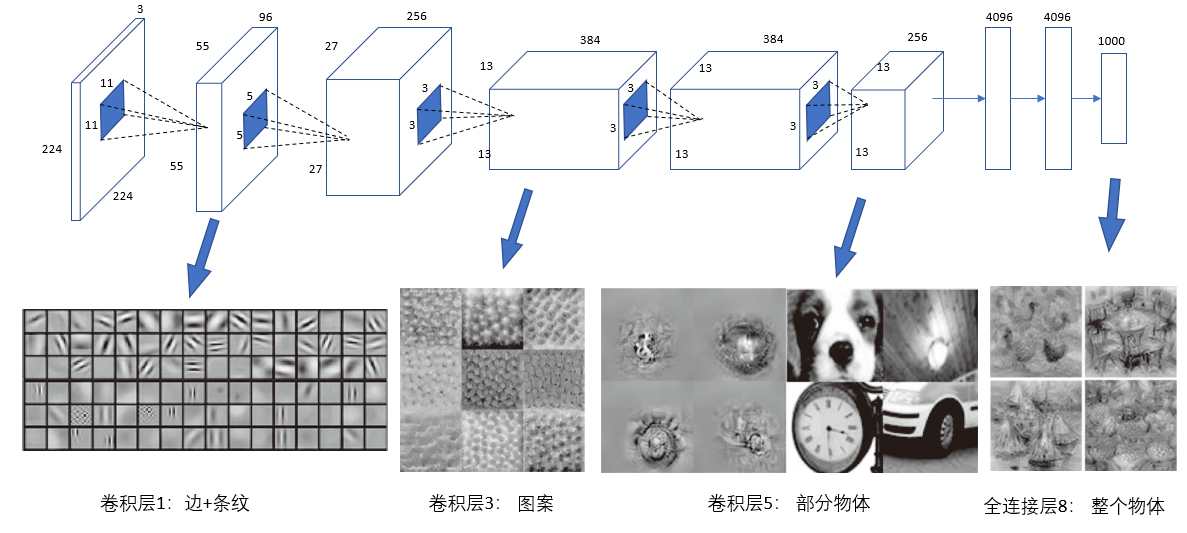
\includegraphics[width=0.9\linewidth]{chapter3_13.png}
    \caption{卷积神经网络的分层抽象特性示意图}
    \label{fig:chapter3_13}
\end{figure}


我们用一个手写两层卷积运算过程的例子来举例说明这种抽象特性。
如图\ref{fig:chapter3_15}所示,图中分为上下两个部分,这两个部分使用两个相同卷积核进行卷积运算,输入数据为图片最左端的的矩阵。$\ast$符号代表卷积运算。将两个卷积运算的结果相加得到了第一卷积层的输出结果。
下面一层也是如此,输入数据经过与两个卷积核运算以后,将运算结果相加,便得到了第一卷积层的输出结果。经过仔细观察后,这张图片的两个卷积核具有明显的特征,上面的卷积核用于提取主对角线的特征,下面的卷积核主要提取次对角线的特征。这些都是较为基本的特征。
经过两个卷积核特征提取后,再将计算结果相加,就得到了两个卷积核特征的相加结果。
\begin{figure}
    \centering
    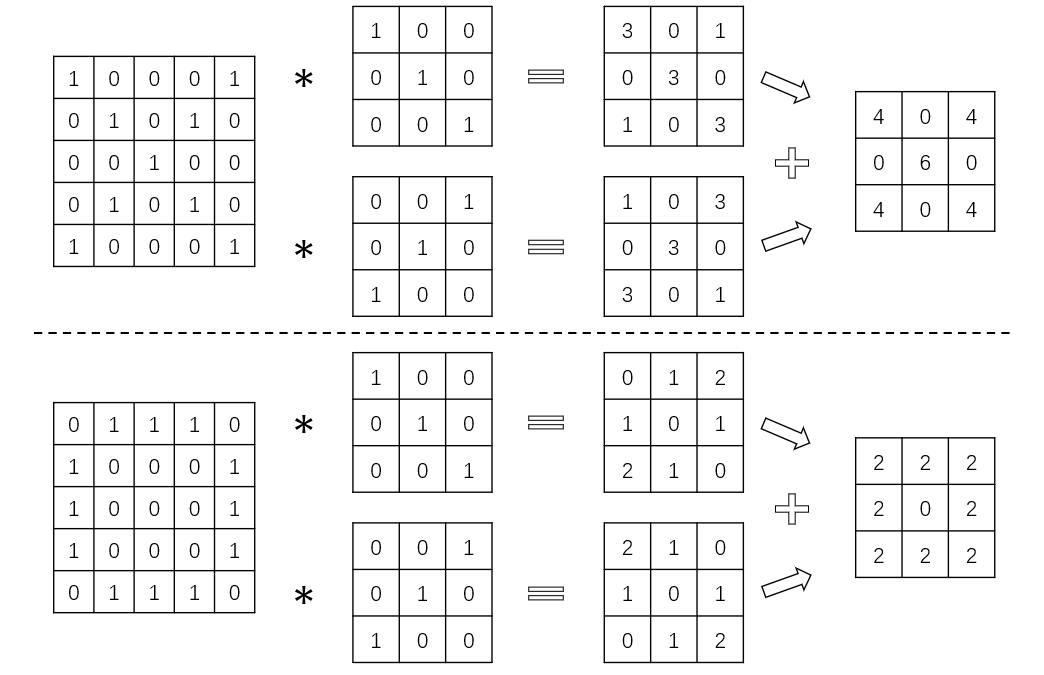
\includegraphics[width=0.9\linewidth]{chapter3_15.png}
    \caption{手写卷积运算示意图1}
    \label{fig:chapter3_15}
\end{figure}

将图\ref{fig:chapter3_15}的输出结果分别再使用两个卷积核进行卷积运算。运算之后分别得到两个运算结果,如图\ref{fig:chapter3_16}所示。
左右两图中分别有两个卷积核,这两个卷积核是对应相等的。仔细观察后可以发现,上面的卷积核主要提取的特征是X形特征的信息;而下面的卷积核主要用于提取O形特征的信息。
图\ref{fig:chapter3_16}(a)中两个卷积运算的结果分别是22和10,这说明图\ref{fig:chapter3_15}上面的输入图片相比于下面的图片更像X形。图\ref{fig:chapter3_16}(b)中两个卷积运算的结果分别是8和16。
这说明图\ref{fig:chapter3_15}下面的输入图片相比于上面的图片更像O形。
相似的结论我们通过肉眼比较也可以得出。通过此例可以明显地感觉到较高层次卷积核的感受野比低层次卷积核的感受野更大。第一卷积层卷积核的感受野是3乘3的方形区域,第二卷积层的感受野是整张图片,即5乘5的方形区域。
由此可见,较高层次的卷积核往往更加关注提取较为抽象的信息,较低层次的卷积核更加关注提取较为基本的信息。
\begin{figure}
    \centering
    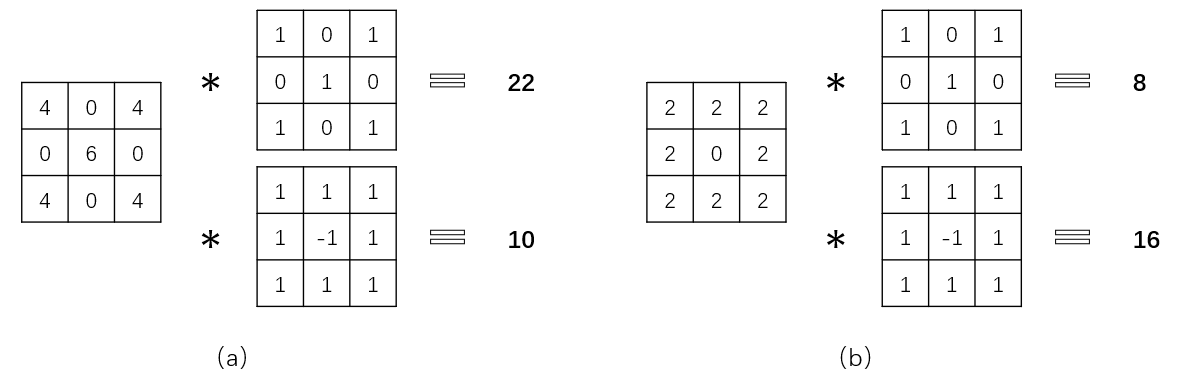
\includegraphics[width=1\linewidth]{chapter3_16.png}
    \caption{手写卷积运算示意图2}
    \label{fig:chapter3_16}
\end{figure}

\section{卷积神经网络遗忘方法介绍}
本节首先介绍遗忘方法的基本思路,然后再讨论遗忘方法的具体步骤。
\subsection{遗忘方法思路}
对一个已经使用数据训练过的神经网络而言,其理想的遗忘效果是,就好像这个神经网络模型从来没有使用要遗忘的数据训练过一样。对于一个用户来说,他不希望自己的数据能够被攻击者窃取或被还原。
当前针对神经网络的攻击方法多种多样,我们与其针对每种攻击方法去设置防御方案,倒不如直接遗忘神经网络模型中指定数据的信息。我们遗忘的信息越多,攻击者得到的信息就越少。遗忘信息的完美情况就是重新训练。
然而重新训练的代价是十分巨大的,一个神经网络模型少则几千个参数,多则高达数亿参数,重新训练的代价是十分昂贵的。所以完全遗忘所有信息看起来是不现实的,我们能做的是尽可能地接近完美情况。
受到卷积神经网络分层抽象特性的启发,我们可以仅遗忘较为抽象的信息,保留一些基本的信息。就像人类视觉信息处理过程一样,卷积神经网络较低层次的卷积层只提取了较为基本的视觉元素,比如边、角、简单的条纹等等。
随着网络层次的提高,抽象程度逐渐提高,比如提取到一些有固定模式的组织,图案等。到卷积神经网络比较高的层次后,卷积核能提取到跟分类息息相关的本质特征,比如不同人脸的区分,以及不同物体的区分,例如猫和狗,飞机和卡车等。
一些基本的特征即使不用窃取,攻击者也能通过类似的模型训练中还原出来。所以攻击者最想获取到的是和分类有关的本质特征信息,而不是基本特征信息。
我们利用这个思路想出了一个既可以遗忘信息,又能不用训练全部参数的折中方案:重置卷积神经网络中靠近输出若干层次的网络参数,再用没有被遗忘的训练集去训练模型,直至模型收敛,同时在训练过程中保持参数没有被重置的层次始终处在冻结状态。
具体过程如图\ref{fig:chapter3_14}所示。
\begin{figure}
    \centering
    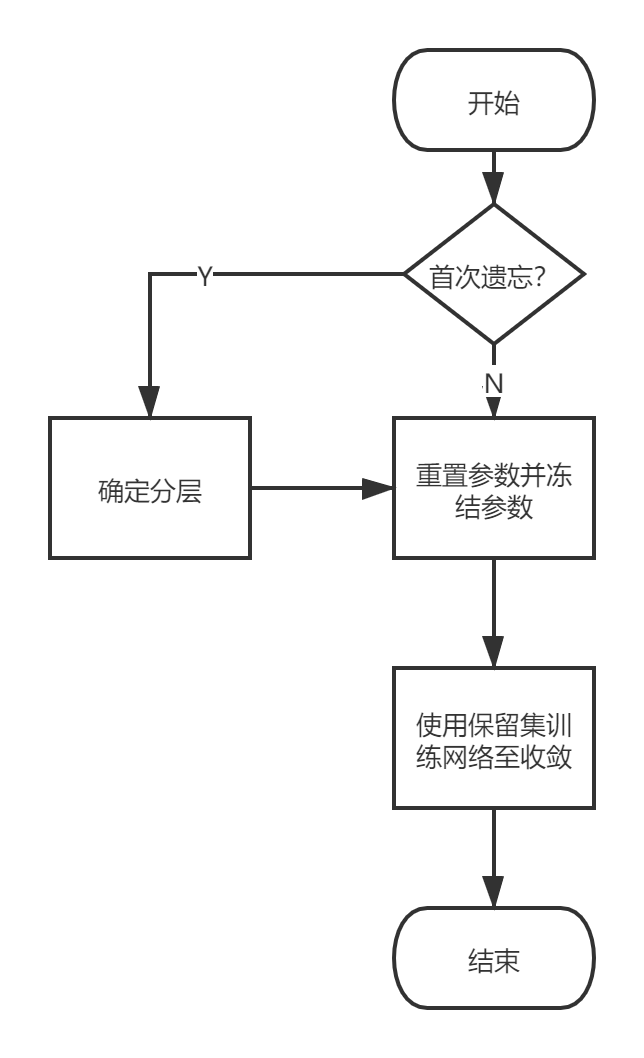
\includegraphics[scale=0.25]{chapter3_14.png}
    \caption{遗忘方法流程图}
    \label{fig:chapter3_14}
\end{figure}

本文主要讲遗忘方法,因此为了表述方便,我们定义需要遗忘的训练数据集为遗忘训练集,原来的训练数据集除去遗忘训练集后称为保留训练集。与数据集的定义类似,在本文我们称要遗忘的类别为遗忘类别,所有类别除去遗忘类别称为保留类别。
测试集中标签是遗忘类别的测试数据组成的集合称为遗忘测试集,由标签是保留类别所组成的测试数据集称为保留测试集。

\subsection{确定分层}
确定如何分层是本方法的一个重要环节,因为重置层数的多少直接影响了遗忘效果的好坏以及重新训练的时间。为了确定分层,我们分两个步骤来进行:第一步是分层预选,第二步是分层评估,下面将分别介绍。

分层的第一步是分层预选,其目的是先找出可能适合分层的层次,排除掉不适合分层的层次。具体方法是通过反向重置冻结参数训练的方法来寻找预选分层。
如图\ref{fig:chapter3_reverse_freeze_1}所示,仍然以8层的AlexNet网络为例。卷积神经网络训练好以后,将其参数分成前后两个部分,分开的方法是从离输入层最近的层次开始分起,离输入层最近的层次作为前面层次,其余所有层次作为后面层次。
\begin{figure}
    \centering
    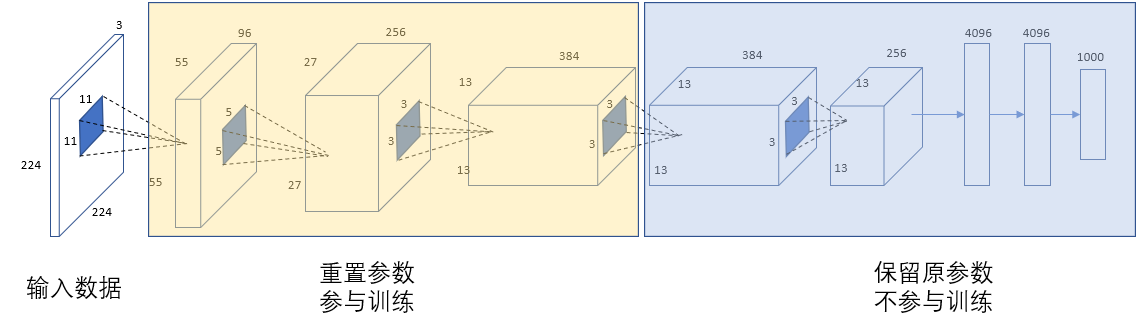
\includegraphics[scale=0.4]{chapter3_reverse_freeze_1.png}
    \caption{反向重置冻结训练方法示意图}
    \label{fig:chapter3_reverse_freeze_1}
\end{figure}
然后,将前面层次的参数初始化成该网络训练之前的对应层次的参数,后面的层次仍然保留原有的参数不变。
最后,将原来的数据集分成两个部分,第一部分仅包含遗忘类别的训练数据,第二部分仅包含保留类别的训练数据。然后用仅包含保留类别的训练数据重新训练网络,直到网络收敛为止,保存训练后的参数。在训练过程中保持只训练前面的参数,后面的参数不参与训练。
经过上述步骤以后,我们再将离输入层较近的两层作为前面的层次,其余层次作为后面的层次。再进行上述步骤,直到网络收敛并保存训练后的参数。以此类推,直到前面参数为全部的参数为止,此时后面的参数为空。

具体方法如算法\ref{algorithm:reverseReset}所示。算法的输入有网络模型的总层数、要遗忘类别的集合、包含所有类别的训练集和测试集。算法最终输出生成模型分别在保留集和遗忘集上准确率的集合。
前两个步骤的作用是初始化神经网络模型并且保存初始化参数,以备后续重置参数时使用。3到4行初始化了两个数组,分别是用于保存保留测试集准确率的数组和用于保存遗忘测试集准确率的数组。
第5行是根据算法\ref{algorithm:dispartDataset}将所有的训练集和所有的测试集根据遗忘的类别分别分成两个部分,一部分只包含遗忘类别的数据,另一部分只包含保留类别的数据。
对于训练集,这两个部分分别称作保留训练集($D_{retain\_train}$)、遗忘训练集($D_{forget\_train}$);对于测试集,这两个部分分别称为保留测试集($D_{retain\_test}$)、遗忘测试集($D_{forget\_test}$)。

\begin{algorithm}
	\renewcommand{\algorithmicrequire}{\textbf{Input:}}
	\renewcommand{\algorithmicensure}{\textbf{Output:}}
	\caption{反向冻结算法 reverseReset}
	\label{algorithm:reverseReset}
	\begin{algorithmic}[1]
        \REQUIRE 模型总层数$totalLayers$,遗忘类别$C_{forget}$,全部训练集$D_{all\_train}$,全部测试集$D_{all\_test}$
        \ENSURE  重置各层的准确率$accRetainArr$和$accForgetArr$
        \STATE $net \gets Initial\ Network$
        \STATE $modelInit \gets net.saveModel()$
        \STATE $accRetainArr \gets []$
        \STATE $accForgetArr \gets []$
        \STATE $D_{retain\_train}, D_{forget\_train}, D_{retain\_test}, D_{forget\_test} \gets dispartDataset(D_{all\_train}, D_{all\_test}, C_{forget})$ (算法\ref{algorithm:dispartDataset})
        \STATE $modelNormal,\_ \gets trainNet(modelInit, trainset, [], T_{threshold})$ (算法\ref{algorithm:trainNet})
        \STATE $modelRetrain,\_ \gets trainNet(modelInit, D_{retain\_train}, [], T_{threshold})$ (算法\ref{algorithm:trainNet})
        \STATE $P_{freeze} \gets []$
        \FOR {$i \to totalLayers$}
            \FOR {$j \to net.params.length$}
                \IF {$net.params[j].layer \leq i$}
                    \STATE $P_{freeze}.push(net.params[j].name)$
                \ENDIF
            \ENDFOR
            \STATE $modelResetBeforeTrain\_i \gets mergeModel(modelInit, modelNormal, totalLayers, totalLayers - i)$  (算法\ref{algorithm:mergeModel})
            \STATE $modelResetAfterTrain\_i \gets$ $trainNet(modelResetBeforeTrain\_i , D_{retain\_test}, P_{freeze}, T_{threshold})$  (算法\ref{algorithm:trainNet})
            \STATE $accRetain \gets getAcc(modelResetAfterTrain\_i, D_{retain\_test})$ (算法\ref{algorithm:getAcc})
            \STATE $accForget \gets getAcc(modelResetAfterTrain\_i, D_{forget\_test})$(算法\ref{algorithm:getAcc})
            \STATE $accRetainArr.push(accRetain)$
            \STATE $accForgetArr.push(accForget)$
        \ENDFOR
        \RETURN $accRetainArr, accForgetArr$
	\end{algorithmic}  
\end{algorithm}
% \begin{algorithm}
% 	\renewcommand{\algorithmicrequire}{\textbf{Input:}}
% 	\renewcommand{\algorithmicensure}{\textbf{Output:}}
% 	\caption{反向冻结算法-内循环 reverseResetInnerCycle}
% 	\label{algorithm:reverseResetInnerCycle}
% 	\begin{algorithmic}[1]
%         \REQUIRE 模型总层数$totalLayers$,初始化参数层数$i$,遗忘类别$C_{forget}$,保留测试集$D_{retain\_test}$,遗忘测试集$D_{forget\_test}$,训练完成模型$modelNormal$,初始化模型$modelInit$
%         \ENSURE  $accReverseRetain\_i, accReverseForget\_i  $

% 		\STATE $modelResetBeforeTrain\_i \gets mergeModel(modelInit, modelNormal, totalLayers, totalLayers - i)$
% 		\STATE $modelResetAfterTrain\_i \gets$ \\
%          $trainNet(modelResetBeforeTrain\_i , D_{retain\_test}, P_{freeze}, T_{threshold})$ 
% 		\STATE $accReverseRetain\_i \gets getAcc(modelResetAfterTrain\_i, D_{retain\_test})$
% 		\STATE $accReverseForget\_i  \gets getAcc(modelResetAfterTrain\_i, D_{forget\_test})$
% 	\end{algorithmic}  
% \end{algorithm}

生成模型的具体方法如算法\ref{algorithm:mergeModel}所示。
\begin{algorithm}
	\renewcommand{\algorithmicrequire}{\textbf{Input:}}
	\renewcommand{\algorithmicensure}{\textbf{Output:}}
	\caption{模型组合算法 mergeModel}
	\label{algorithm:mergeModel}
	\begin{algorithmic}[1]
        \REQUIRE 前部分重置的模型$formerModel$,后部分重置的模型$laterModel$,模型总层数$totalLayers$,后部分重置的层数$resetLayerCount$
        \ENSURE  $mergedModel$
        \FOR {$i \to resetLayerCount$}
            \STATE $formerModel[totalLayers - i] \gets laterModel[totalLayers - i]$
        \ENDFOR
        \STATE $mergedModel \gets formerModel$
        \RETURN $mergedModel$
	\end{algorithmic}  
\end{algorithm}

经过上述过程之后,我们将得到和网络层数相同的训练好的模型。然后分别测量这些网络在遗忘测试数据集上的准确率,然后绘制准确率曲线。绘制的准确率曲线大致趋势如图\ref{fig:chapter3_reverse_freeze_2}所示。
\begin{figure}
    \centering
    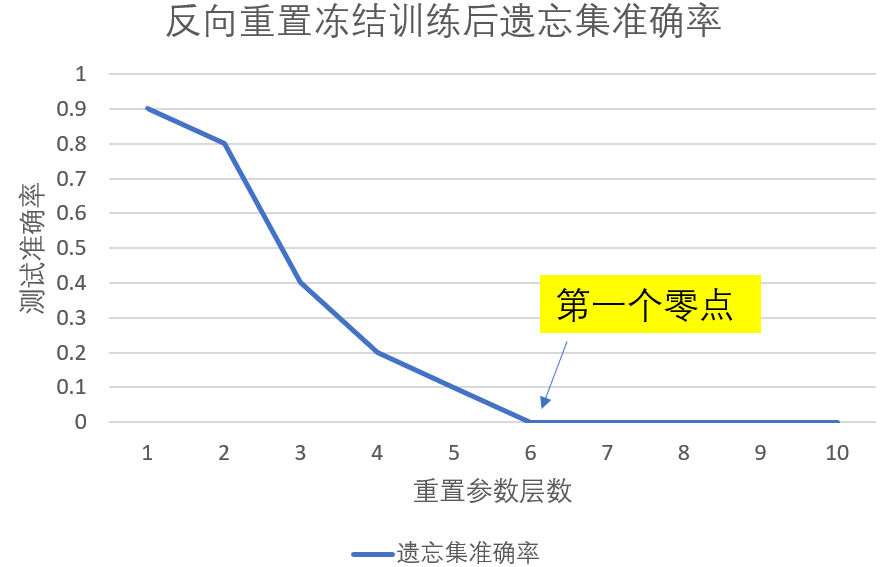
\includegraphics[scale=0.4]{chapter3_reverse_freeze_2.png}
    \caption{反向重置冻结训练后遗忘准确率曲线}
    \label{fig:chapter3_reverse_freeze_2}
\end{figure}
图中展示了反向重置训练后遗忘测试集准确率的大致曲线。重置参数层数较少时,遗忘集测试准确率仍然有较高的数值,说明需要遗忘的数据并没有被遗忘。直到某个点接近零后,后面所有的层次全部为零。我们称第一个近似为零的点为“第一个零点”。
这也是我们预选分层的地方。我们将“第一个零点”的位置作为我们确定分层的预选位置。于是,我们就完成了确定分层的第一个步骤。

预选分层以后,我们仍然不能确定实施该分层后的遗忘效果。为了更好地确定分层,我们进行确定分层的第二个步骤,分层评估。其具体做法是通过正向重置冻结训练的方法测试各个层次的评价指标,然后综合这些评价指标来最终确定分层。
正向重置冻结参数训练的方法如图\ref{fig:chapter3_reset_freeze}所示。首先,将网络参数分成前后两个部分。分开的方法仍然是逐层进行。
第一次先将离输出层最近的一层作为后面层次,其余层次作为前面层次。第二次将离输出层最近的两层作为后面层次,其余层次作为前面层次。以此类推,直到所有层次均作为后面层次,前面层次为空为止。
然后,将后面的层次初始化,将前面的层次保持原有状态不动。
最后,将原来的数据集分成两个部分,第一部分仅包含遗忘类别的数据,第二部分仅包含保留类别的数据。使用仅包含保留类别的数据去训练重置参数后的模型,直到模型收敛为止。在训练过程中,保持前面层数保持冻结,不参与参数更新过程。
\begin{figure}
    \centering
    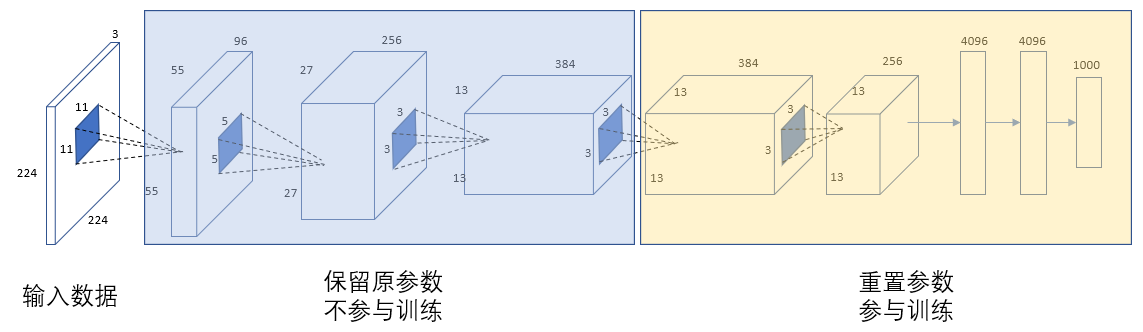
\includegraphics[scale=0.4]{chapter3_reset_freeze.png}
    \caption{正向重置冻结训练方法示意图}
    \label{fig:chapter3_reset_freeze}
\end{figure}
其具体过程如算法\ref{algorithm:normalResetMain}所示。
\begin{algorithm}
	\renewcommand{\algorithmicrequire}{\textbf{Input:}}
	\renewcommand{\algorithmicensure}{\textbf{Output:}}
	\caption{正向冻结算法-外循环 normalResetMain}
	\label{algorithm:normalResetMain}
	\begin{algorithmic}[1]
        \REQUIRE 模型总层数$totalLayers$,遗忘类别$C_{forget}$,全部测试集$D_{all\_train}$,全部测试集$D_{all\_test}$,初始网络模型$net$
        \ENSURE  $accNormalFreezeRetainArr,accNormalFreezeForgetArr,$\\$distanceNormalFreezeRetainArr,distanceNormalFreezeForgetArr,T_{convergeArr}$
        \STATE $accNormalFreezeRetainArr,accNormalFreezeForgetArr,$\\$distanceNormalFreezeRetainArr,distanceNormalFreezeForgetArr,T_{convergeArr} = []$
        \STATE $D_{retain\_train}, D_{forget\_train}, D_{retain\_test}, D_{forget\_test} \gets dispartDataset(D_{all\_train}, D_{all\_test}, C_{forget})$(算法\ref{algorithm:dispartDataset})
        \STATE $modelInit \gets net.saveModel()$
        \STATE $modelNormal,\_ \gets trainNet(modelInit, trainset, P_{freeze}, T_{threshold})$(算法\ref{algorithm:trainNet})
        \STATE $modelRetrain,\_ \gets trainNet(modelInit, D_{retain\_train}, [], T_{threshold})$(算法\ref{algorithm:trainNet})
        \FOR {$i \to totalLayers$}
            \STATE $accNormalFreezeRetain\_i,accNormalFreezeForget\_i,$\\
            $distanceNormalFreezeRetain\_i,distanceNormalFreezeForget\_i,T_{converge\_i} \gets normalFreezeResetInnerCycle(totalLayers, i, C_{forget}, D_{retain\_train}, D_{retain\_test}, D_{forget\_test}, $\\$modelRetrain)$(算法\ref{algorithm:normalFreezeResetInnerCycle})
            \STATE $accNormalFreezeRetainArr.push(accNormalFreezeRetain\_i)$
            \STATE $accNormalFreezeForgetArr.push(accNormalFreezeForget\_i)$
            \STATE $distanceNormalFreezeRetainArr.push(distanceNormalFreezeRetain\_i)$
            \STATE $distanceNormalFreezeForgetArr.push(distanceNormalFreezeForget\_i)$
            \STATE $T_{convergeArr}.push(T_{converge\_i})$
        \ENDFOR
        \RETURN $accNormalFreezeRetainArr,accNormalFreezeForgetArr,$\\$distanceNormalFreezeRetainArr,distanceNormalFreezeForgetArr,T_{convergeArr}$
	\end{algorithmic}  
\end{algorithm}
\begin{algorithm}
	\renewcommand{\algorithmicrequire}{\textbf{Input:}}
	\renewcommand{\algorithmicensure}{\textbf{Output:}}
	\caption{正向冻结算法-内循环 normalFreezeResetInnerCycle}
	\label{algorithm:normalFreezeResetInnerCycle}
	\begin{algorithmic}[1]
        \REQUIRE 模型总层数$totalLayers$,初始化参数层数$i$,遗忘类别$C_{forget}$,保留训练集$D_{retain\_train}$,保留测试集$D_{retain\_test}$,遗忘测试集$D_{forget\_test}$,对比模型$modelCmp$
        \ENSURE  $accNormalFreezeRetain\_i,accNormalFreezeForget\_i,$\\$distanceNormalFreezeRetain\_i,distanceNormalFreezeForget\_i,T_{converge\_i}$
		\STATE $modelResetBeforeTrain\_i \gets mergeModel(modelNormal, modelInit, totalLayers, i)$(算法\ref{algorithm:mergeModel})
        \STATE $modelResetAfterTrain\_i,T_{converge\_i} \gets trainNet(modelResetBeforeTrain\_i , D_{retain\_train},$\\$ P_{freeze}, T_{threshold})$(算法\ref{algorithm:trainNet})
        \STATE $accNormalFreezeRetain\_i \gets getAcc(modelResetAfterTrain\_i, D_{retain\_test})$(算法\ref{algorithm:getAcc})
        \STATE $accNormalFreezeForget\_i  \gets getAcc(modelResetAfterTrain\_i, D_{forget\_test})$(算法\ref{algorithm:getAcc})
        \STATE $distanceNormalFreezeRetain\_i \gets getDistance(model, modelCmp, D_{retain\_test})$(算法\ref{algorithm:getDistance})
        \STATE $distanceNormalFreezeForget\_i \gets getDistance(model, modelCmp, D_{forget\_test})$(算法\ref{algorithm:getDistance})
        \RETURN $accNormalFreezeRetain\_i,accNormalFreezeForget\_i,$\\$distanceNormalFreezeRetain\_i,distanceNormalFreezeForget\_i,T_{converge\_i}$
	\end{algorithmic}  
\end{algorithm}

训练好模型后,我们将得到和参数层数数量相同的模型。分别测试这些模型的相应指标:首先是准确率。准确率分为两大类,一类是只使用遗忘数据集测试的遗忘测试准确率,另一类则是只使用保留数据集测得的保留测试准确率。
选择这个指标是出于实际应用的考虑。因为我们训练神经网络模型的目的是用于分类,所以一个最基本的要求就是要在保留的数据集上有较高的分类准确率,在遗忘的数据集上要有和重新训练的模型类似的准确率。
其次是重新训练时间,这也是十分重要的指标。重新训练时间如果长于完全重新训练的时间,那么本方法就没有了存在的价值。
有了上述确定分层的指标,我们就可以对分层结果进行评价。具体的评价原则是:首先,尽可能地接近预选层数。其次,对于遗忘类别准确率尽可能为0,对于保留类别准确率尽可能地高。对于收敛时间,要尽可能地低。
尽可能地接近预选层数是为了保证遗忘的效果。因为通过实验我们发现虽然重置较后面的层次能够达到较高的保留准确率和较低的遗忘准确率和较快的收敛时间,但是并不能保证激活距离与完全重新训练保持足够的接近。
实验数据表明,重置参数层数越多,激活距离越接近。预选层数可以满足这一要求,通过预选层数,我们可以知道到了哪一层才与最终的分类直接相关。尽可能地接近预选层数,也就是要尽可能多地重置与分类相关的层次。
再有,通过考虑遗忘准确率、保留准确率还有收敛时间,我们可以保证遗忘后的使用效果和训练过程时间的可控。

需要说明的一点是,在本方法中我们无需在每次遗忘时均确定分层,仅需在首次使用时确定分层。实验结果表明,确定一次分层可以很好地支持神经网络进行连续的遗忘操作。
在实际寻找预选层次过程中,我们无需对网络的每一个层次均进行测试,可以使用二分查找的方法来加速查找过程。
比如使用一个层数为10层的卷积神经网络时,假设“第一次零点”是从输入层开始的第四层。我们可以先查找第5层,因为第5层的遗忘准确率为0,我们再利用一次二分查找,这次是第3层。
结果发现第3层的遗忘集准确率不为0,再利用一次二分查找,这次是第4层。当我们发现第4层的遗忘测试准确率为0时,我们就能确定预选层数是第4层,这可以使得预选层数的查找算法复杂度从$O(n)$降到$O(\log n)$。

\subsection{重置并冻结参数}
确定好如何分层后,就要重置从分层点开始到输出层的所有参数,并且将没有被重置的参数冻结,防止在训练中被更新。重置并冻结参数的原因是为了减少遗忘数据在原网络中的信息,并且保留和分类关系不密切的基本信息。
对于重置和冻结参数,我们将分开进行解释。

重置参数就是将一些层次的参数使用另外一些数值代替。如果替代的参数选择不当,可能会导致模型无法收敛,或导致无法达到全局最优等问题。
为了防止这样的由于参数初始化不当而带来的问题,我们选取的策略是,保存模型的初始化参数。当网络中某些层次需要重置参数时,我们将保存下来的相应层次最初的网络参数补充到需要重置参数的层次当中。
这样做的原因是,既然这个网络模型初始化参数能够使得网络达到收敛状态,就说明这个参数是一个较为合理的初始化参数,没有均值过大或过小,方差过大或过小的异常情况。
经过实验证明,这种做法能够达到理想的效果,在实验中并未发现由于重置参数不当而带来的网络训练无法收敛的问题。

对于冻结网络,需要关注的问题是冻结网络的必要性。为了探究是否有必要冻结参数,本文设计了冻结参数与非冻结参数的对比实验,实验过程和结果将在下一章中展示。

\subsection{训练网络}
重置并冻结参数后,我们要使用保留集继续训练被重置的参数,直至网络再次收敛。再次训练网络时,使用的数据集是保留训练集。
重新训练网络的目的是为了还原保留类别的信息。因为重置了一部分网络参数后,所有的训练数据中涉及到的分类信息已经全被消除掉了。
此时网络攻击者根据网络输出还原训练数据的信息几乎是不可能的。为了保证保留类别还原重置参数以前的效果,我们使用保留集对重置的参数进行还原。

在重新训练网络的过程中,待更新的参数数量对比完全重新训练的参数数量,少了冻结层次的参数,因此训练网络中不需要对冻结的参数计算梯度。
从理论上看,训练参数的降低将加快网络参数的收敛速度。为了检验收敛速度提升情况,我们专门设计了对比实验,分别记录完全重新训练所花费的训练批次数和使用本文遗忘方法训练所需要花费的训练批次数。

\section{遗忘效果的衡量指标} \label{forget_evaluation_index}
在本节,我们引用了一些用来评价遗忘效果的指标。这些指标可以帮助我们从各个方面了解当前网络模型的遗忘状态。具体有三个指标,分别是测试准确率、收敛时间和激活距离。

\subsection{测试准确率}
训练神经网络的过程中,我们不仅要利用训练数据去训练网络,也需要用测试集去测试训练网络的泛化成果,目的是为了检测训练的网络是否出现过拟合情况。我们将测试集根据遗忘需求分为两个部分,仅有遗忘类别的遗忘测试集和仅有保留类别的保留测试集。
使用遗忘测试集的测试结果可以反映网络对于遗忘类别的遗忘程度。单从测试准确率这一个指标上来看,使用本文方法遗忘后的网络与完全重新训练后的网络在遗忘测试集的准确率上越接近,遗忘的效果就越好。
同理,使用保留测试集的测试结果可以反映网络对于保留类别的保留情况。单从测试准确率这个指标上来看,在保留测试集上的准确率越高,代表保留类别的保留效果越明显。获取准确率具体方法如算法\ref{algorithm:getAcc}所示。
\begin{algorithm}
	\renewcommand{\algorithmicrequire}{\textbf{Input:}}
	\renewcommand{\algorithmicensure}{\textbf{Output:}}
	\caption{记录测试准确率算法  getAcc}
	\label{algorithm:getAcc}
	\begin{algorithmic}[1]
        \REQUIRE 待测模型$model$,测试集$D_{test}$
        \ENSURE  测试准确率$acc$
        \STATE $total \gets 0$
        \STATE $corrects \gets 0$
        \FOR {$i \to D_{test}$}
            \STATE $inputs, labels \gets D_{test}[i]$
            \STATE $net.loadModel(model)$
            \STATE $outputs \gets net(inputs)$
            \STATE $predict \gets max(outputs.data)$
            \STATE $total \gets total + D_{test}[i].length$
            \FOR{$j \to D_{test}[i].length$}
                \IF{$predict[j] == labels[j]$}
                    \STATE $corrects \gets corrects + 1$
                \ENDIF
            \ENDFOR
        \ENDFOR
        \STATE $acc \gets corrects {\ } / {\ } total$
        \RETURN acc
	\end{algorithmic}  
\end{algorithm}

\subsection{收敛时间}
收敛时间用于衡量本文遗忘方法在时间上的节约程度。规定从用保留集进行训练开始,到当前训练批次损失函数输出的平均值小于一定限值为止,这中间过程的训练批次数称为收敛时间。
这么定义的目的是因为具体的时间间隔会因实验环境的不同而不同,比如实验用的CPU,内存,硬盘,显卡,神经网络结构和数据集等都有可能发生变化。本文使用了两台配置不同的实验主机,因此我们要寻找一个既能反映训练过程长短又能不随实验环境变化的量。
训练批次数刚好符合这个条件,Epoch是训练数据训练完成的轮数。
因此无论训练环境如何变化,只要BATCH\_SIZE(一次批处理运算包含的训练样例个数)和学习率(Learnnig Rate,LR,网络训练过程中的超参数,参数变更的实际大小=计算出变更大小 $\times$ LR)是相同的,使用的时间可能有快有慢,但是训练过程计算的次数是相同的。

为了便于实验结果的对比,我们给收敛时间确定了一个计算公式。我们将收敛时间定义为网络训练过程中,本轮Epoch中平均的损失函数值首次下降到指定阈值时所花费的Epoch数。在本文的实验中取了三个阈值,分别是0.1,0.05和0.03。

将从保留集开始训练的时刻作为起始时间是因为确定分层步骤是一次性的步骤,对于同一个网络结构,确定网络分层仅在第一次遗忘时确定一次,以后遗忘时沿用上次的网络分层即可。

获取收敛时间以及训练网络具体方法如算法\ref{algorithm:trainNet}所示。
\begin{algorithm}
	\renewcommand{\algorithmicrequire}{\textbf{Input:}}
	\renewcommand{\algorithmicensure}{\textbf{Output:}}
	\caption{训练网络与记录收敛时间算法  trainNet}
	\label{algorithm:trainNet}
	\begin{algorithmic}[1]
        \REQUIRE 初始模型$modelInit$,训练数据$Dataset$,冻结参数集合$P_{freeze}$,收敛时间限值$T_{threshold}$
        \ENSURE  $newModel,T_{converge} $
        \STATE $EPOCH \gets init\_hyper\_parameter\_value$
        \STATE $criterion \gets crossEntropyLoss$
        \STATE $T_{converge} \gets null$
        \STATE $net.loadModel(modelInit)$
        \FOR {$i \to net.params.length$}
            \IF {$net.params[i].name \in P_{freeze}$}
                \STATE $net.params[i].requires\_grad \gets True$
            \ENDIF
        \ENDFOR
        \FOR {$epoch \to EPOCH$}
            \STATE $loss\_sum \gets 0$
            \STATE $dataLength \gets Dataset.length$
            \FOR {$j \in dataLength$}
                \STATE $inputs,labels \gets Dataset[j]$
                \STATE $outputs \gets net(inputs)$
                \STATE $loss \gets criterion(outputs, labels)$
                \STATE $loss.backward()$
                \STATE $loss\_sum \gets loss\_sum + loss.value$
            \ENDFOR
            \IF {$(loss\_sum {\ } / {\ } dataLength < T_{threshold}) and (T_{converge} == null)$}
                \STATE $T_{converge} \gets epoch$
            \ENDIF
        \ENDFOR
        \STATE $newModel \gets net.saveModel()$
        \RETURN $newModel, T_{converge}$
	\end{algorithmic}  
\end{algorithm}

\subsection{激活距离}
激活距离是指遗忘后模型与完全重新训练模型在测试集上的平均距离。它用于衡量遗忘后模型与完全重新训练模型在网络输出结果上的相似程度。它的计算公式是
\begin{equation}
I_{distance} = {\mathbb{E}}_{x\in {\mathcal{D}_{test}}}[{\Vert softmax(f_w(x)) - softmax(f_{w_{\mathcal{D}_R}}) \Vert}_2 ] \label{equation:index_distance}
\end{equation}
具体计算方法如算法\ref{algorithm:getDistance}所示。
\begin{algorithm}
	\renewcommand{\algorithmicrequire}{\textbf{Input:}}
	\renewcommand{\algorithmicensure}{\textbf{Output:}}
	\caption{记录激活距离算法  getDistance}
	\label{algorithm:getDistance}
	\begin{algorithmic}[1]
        \REQUIRE 待测模型$model$,对照模型$modelCmp$,保留测试集$D_{test}$
        \ENSURE  激活距离$distance$
        \STATE $normTotal \gets 0$
        \STATE $total \gets D_{test}.length$
        \FOR {$i in D_{test}$}
            \STATE $inputs, labels \gets D_{test}[i]$
            \STATE $net.loadModel(model)$
            \STATE $outputs \gets net(inputs)$
            \STATE $probabilityToTest \gets softmax(outputs)$
            \STATE $net.loadModel(modelCmp)$
            \STATE $outputsTarget \gets net(inputs)$
            \STATE $probabilityTarget \gets softmax(outputsTarget)$
            \STATE $diff \gets probabilityToTest - probabilityTarget $
            \FOR {$i \to diff.length$}
                \STATE $normTotal \gets normTotal + norm(diff[i],2)$
            \ENDFOR
        \ENDFOR
        \STATE $distance \gets normTotal {\ } / {\ } total$
        \RETURN $distance$
	\end{algorithmic}  
\end{algorithm}

$f_w(x)$代表完全重新训练网络的输出结果,$f_{w_{\mathcal{D}_R}}$代表使用本文遗忘方法训练网络的输出结果。
两个模型输出结果Softmax函数输出的差值向量的第二范数在测试集上的期望就是激活距离。


\section{本章小结}
本章对本文所使用的遗忘方法做了系统性的描述。为了讲清卷积神经网络的分层抽象特性,本章首先介绍了卷积神经网络技术的基本原理,包括卷积操作以及卷积层和池化层的作用。
其次依托于生物视觉信息处理过程和手写卷积运算的例子,介绍了卷积神经网络的分层抽象特性,这也是本文所使用方法的理论依据。
然后分步骤介绍了本文所使用的遗忘方法。本文遗忘方法可以分为三个步骤:确定冻结层次、重置并冻结参数和训练网络。最后介绍了本文用来评价遗忘效果的主要指标,包括测试准确率、收敛时间和激活距离。

% !TeX root = ../thuthesis-example.tex

\chapter{遗忘方法的实现与验证}

\section{实验介绍}

\subsection{实验环境介绍}
我们用到的实验设备是两台服务器,如表\ref{tab:experiment-deivce}所示。
\begin{table}
    \centering
    \caption{实验设备情况}
    \begin{tabular}{lll}
      \toprule
      属性  & 设备1 & 设备2  \\
      \midrule
      CPU   & Core(TM) i9-9900K CPU @ 3.60GHz & Core(TM) i7-6700K CPU @ 4.00GHz \\
      内存大小  & 32G & 32G                    \\
      硬盘类型 & SSD  & SSD  \\
      显卡类型 & Nvidia Geforce 2080  & Nvidia Geforce 1080  \\
      显卡数量 & 1  & 3  \\
      操作系统 & Ubuntu 16.04LTS  & Ubuntu 16.04LTS  \\
      Python版本 & 3.8.7  & 3.8.8  \\
      Pytorch版本 & 1.7.1  & 1.8.0  \\
      显卡驱动版本 & 460.56  & 455.23.05  \\
      CUDA版本 & 11.2  & 11.1  \\
      \bottomrule
    \end{tabular}
    \label{tab:experiment-deivce}
\end{table}

我们使用的深度学习框架是Pytorch,数据集是CIFAR-10\cite{cifar10_2009},正常训练集有50000张图片,测试集有10000张图片。这个数据集共有10个类别,每个类别有5000张训练数据和1000张测试数据。
在确定冻结层数实验中,我们默认遗忘两个类别。因此遗忘训练集是从正常训练集分离出来的10000张图片,遗忘测试集2000张图片。保留训练集是指正常训练集除去了遗忘集以外的数据集合。
保留训练集40000张图片,保留测试集8000张图片。我们使用的神经网络框架是Resnet18\cite{He_2016_CVPR},是一个具有代表性的卷积神经网络。

在训练时我们使用了自适应学习率的方法,自适应的策略是如果该轮训练后测试集的准确率连续3次低于历史最好值,则学习率减半。每次训练数量(BATCH\_SIZE)是100,初始学习率(LEARNING\_RATE)为0.1。训练的方法使用随机梯度下降(SGD)训练方法,权重衰减参数(WEIGHT\_DECAY)为0.0005,冲量参数(MOMENTUM)为0.9。

\subsection{实验设计}
\subsubsection{确定冻结层数实验}
\begin{figure}
    \centering
    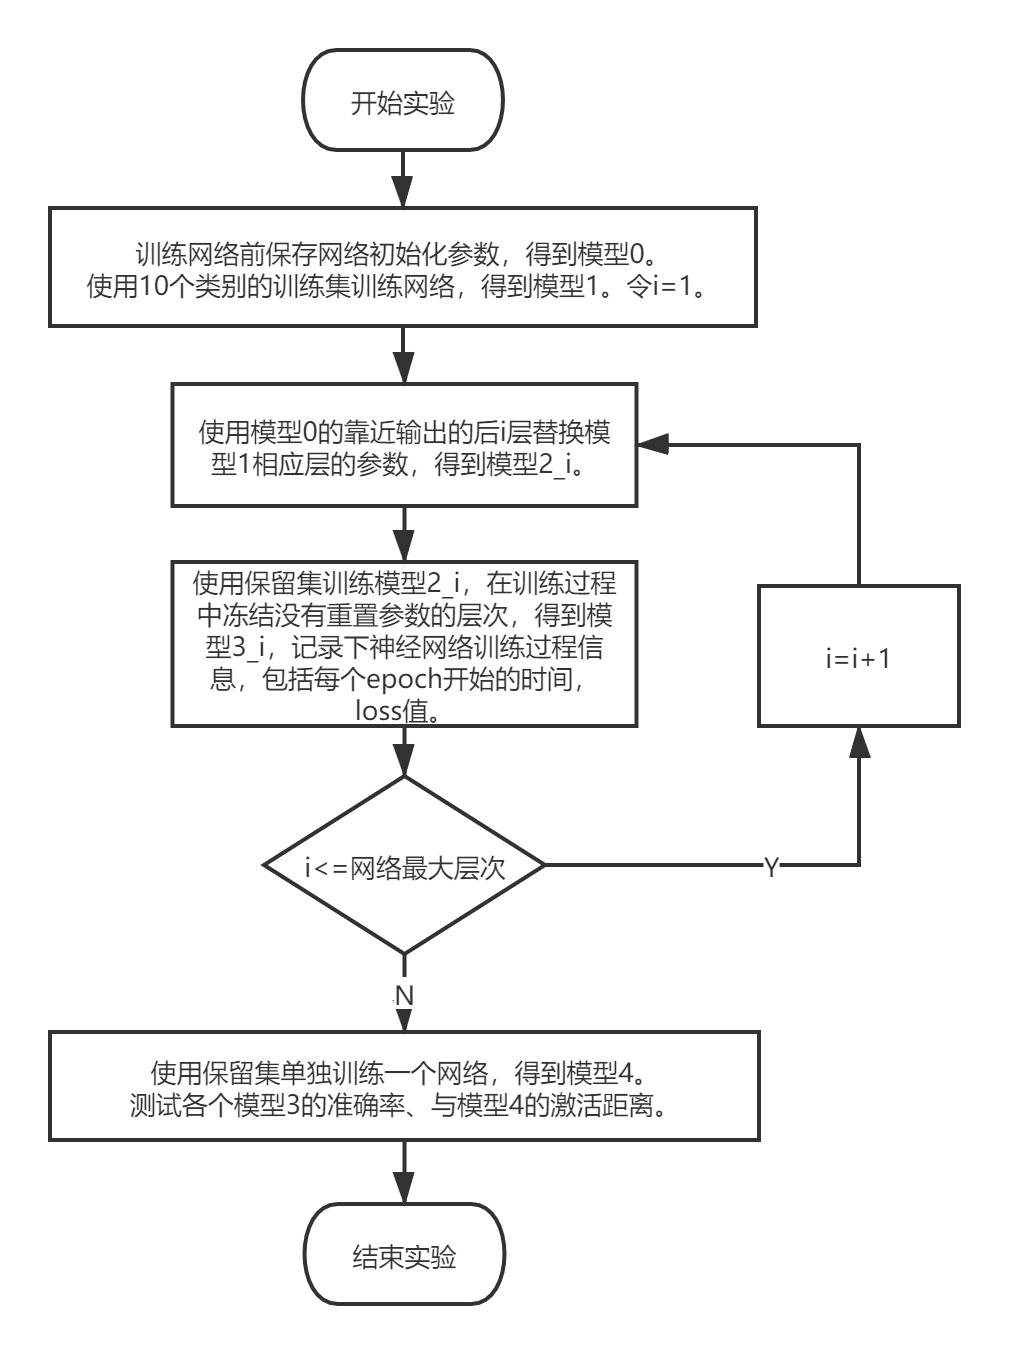
\includegraphics[scale=0.32]{chapter4_process_1.png}
    % 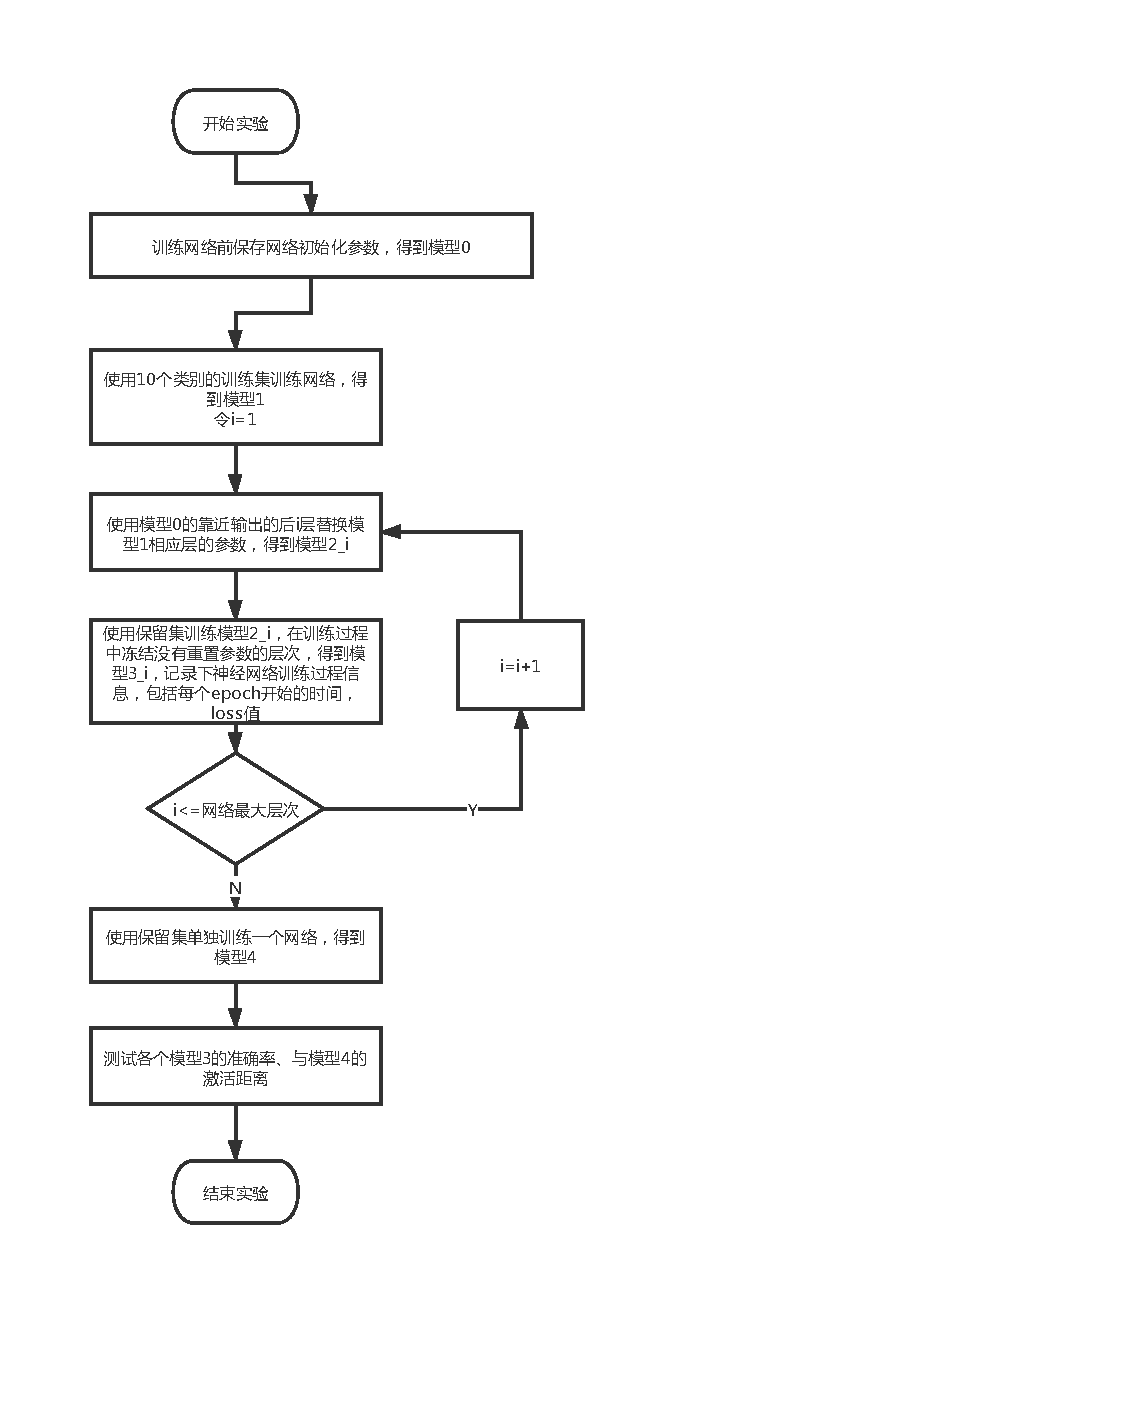
\includegraphics{chapter4_process_1.pdf}
    \caption{确定冻结层数实验流程图}
    \label{fig:chapter4_process_1}
\end{figure}

这个实验的目的是通过实验确定网络冻结的层次数。确定的标准是根据\ref{forget_evaluation_index}章节中介绍的三个指标。具体流程如图\ref{fig:chapter4_process_1}所示。
我们首先使用正常训练集去训练神经网络,直至训练集准确率收敛,获得模型1。在训练网络之前保存神经网络训练的初始参数,记为模型0。
将模型1的最后一层(全连接层)的参数替换为模型0的最后一层参数,模型1其余层数的参数保持不变,由此得到模型2\_1。
将模型2\_1加载到一个新的神经网络中,使用保留训练集去训练这个新的网络,直至训练准确率收敛。在训练过程中保持除全连接层以外层次的参数不被更新(即冻结)。训练收敛后得到模型3\_1。
然后再将模型1的后两层参数替换为模型0的后两层参数,得到模型2\_2。将模型2\_2用保留训练集去训练至模型收敛,训练过程中保持未被重置的参数冻结。模型收敛后得到模型3\_2。
以此类推,逐层重置并冻结参数,使用保留训练集训练至模型收敛。
最后再使用保留训练集完全重新训练一个神经网络,获得模型4。
将每个模型3测量准确率、收敛时间和与模型4的激活距离,根据实验结果综合分析确定冻结层数。

本实验使用的遗忘测试集包含CIFAR10中轮船和卡车的测试数据,保留训练集包含CIFAR10中除了轮船和卡车以外所有的训练数据,保留测试集包含除了轮船和卡车以外所有的测试数据。

\subsubsection{冻结必要性验证实验}
\begin{figure}
    \centering
    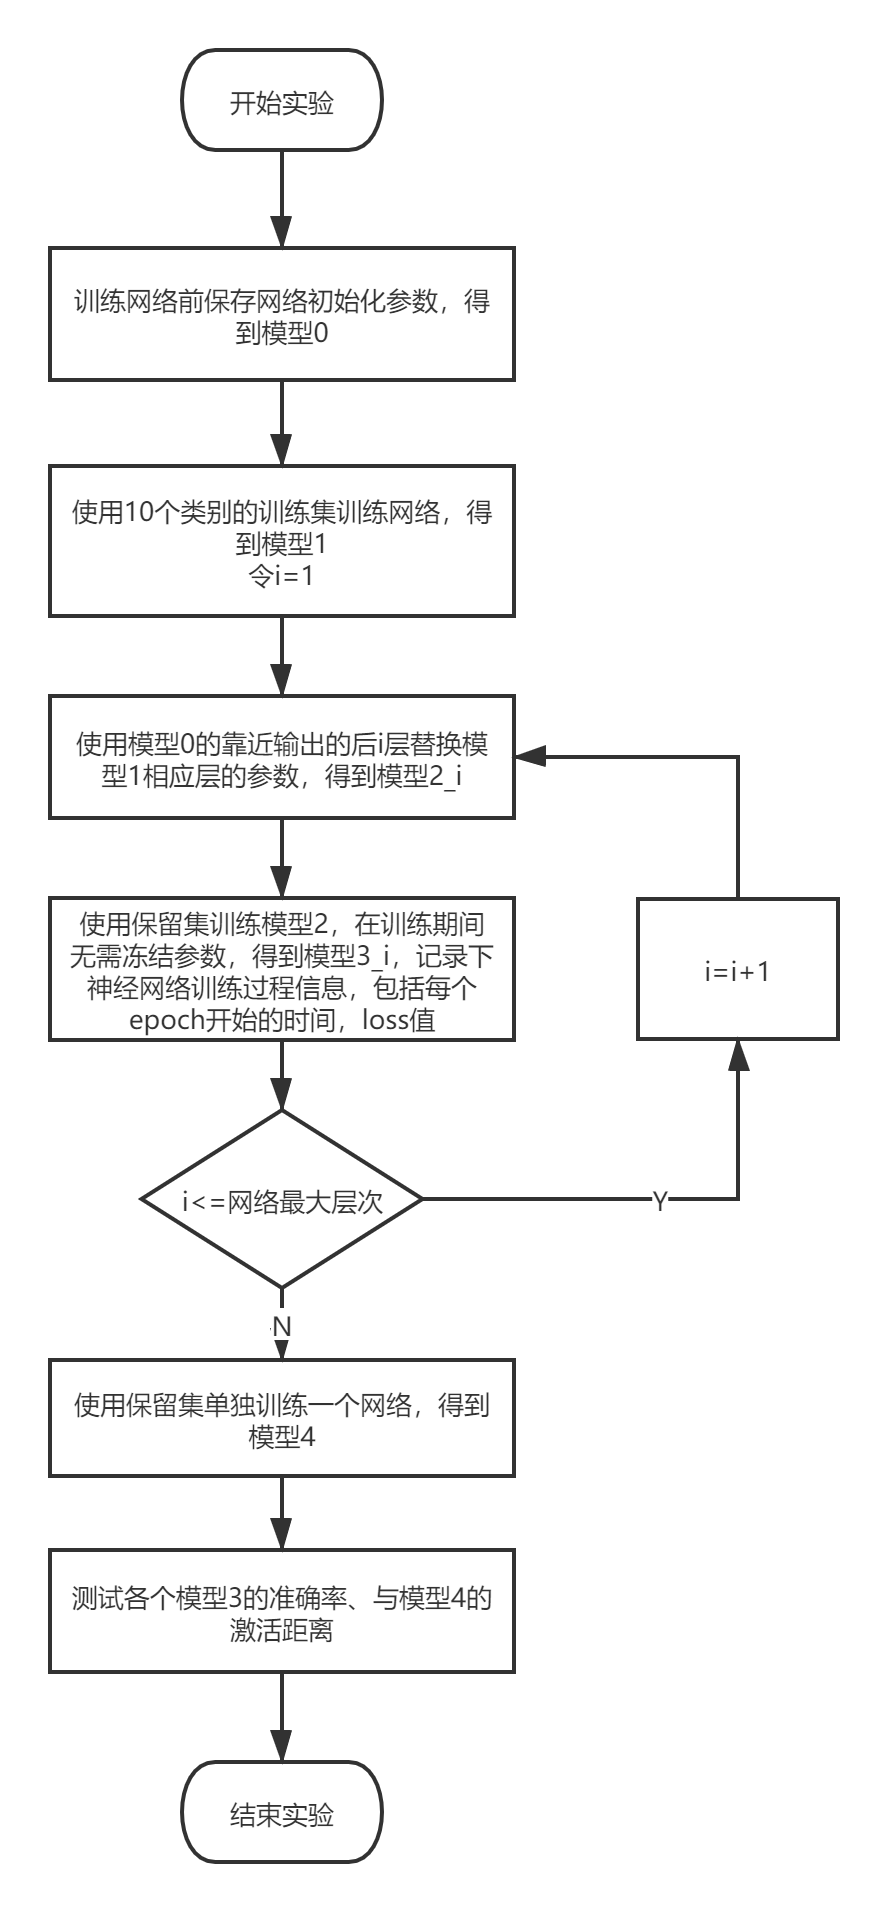
\includegraphics[scale=0.32]{chapter4_process_2.png}
    \caption{冻结必要性实验流程图}
    \label{fig:chapter4_process_2}
\end{figure}

通过本实验可以验证冻结较低层次的参数是否对加快遗忘训练收敛速度有一定的贡献。
本实验的实验过程和确定冻结层数实验大致相同。不同的地方在于训练模型至收敛的过程中无需冻结参数,以对比冻结参数对遗忘效果的影响程度。如图\ref{fig:chapter4_process_2}所示。
我们首先使用正常训练集去训练神经网络,直至训练集准确率收敛,获得模型1。在训练网络之前保存神经网络训练的初始参数,记为模型0。
将模型1的最后一层的参数替换为模型0的最后一层参数,模型1其余层数的参数保持不变,由此得到模型2\_1。
将模型2\_1加载到一个新的神经网络中,使用保留训练集去训练这个新的网络,直至训练准确率收敛。在训练过程中所有参数都将会得到更新。训练收敛后得到模型3\_1。
然后再将模型1的后两层参数替换为模型0的后两层参数,得到模型2\_2。将模型2\_2用保留训练集去训练至模型收敛,在训练过程中所有参数都将会得到更新。模型收敛后得到模型3\_2。
以此类推,逐层重置并且不冻结参数,使用保留训练集训练至模型收敛。
最后再使用保留训练集完全重新训练一个神经网络,获得模型4。
将模型3\_i测量准确率、收敛时间和与模型4的激活距离,根据实验结果综合测算冻结参数的必要性。

本实验中使用的遗忘测试集、保留训练集和保留测试集均和确定冻结层数实验中的相同。

\subsubsection{反向冻结验证实验}
\begin{figure}
    \centering
    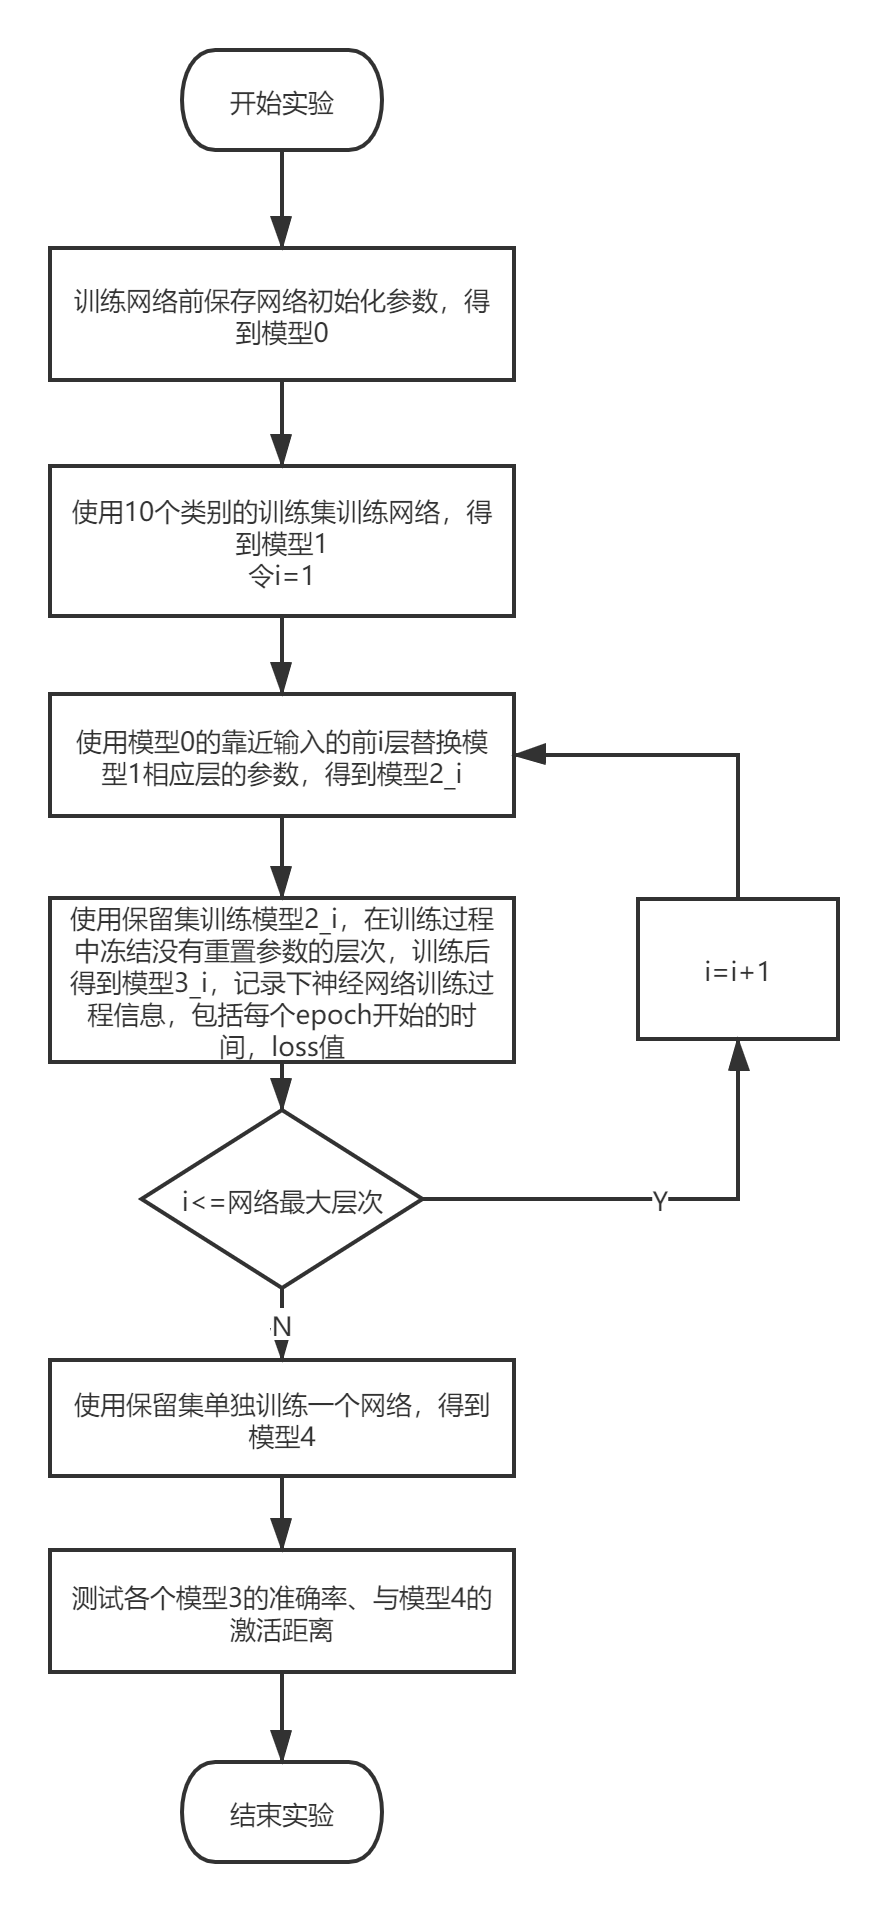
\includegraphics[scale=0.32]{chapter4_process_3.png}
    \caption{反向冻结验证实验流程图}
    \label{fig:chapter4_process_3}
\end{figure}

本实验是为了验证卷积神经网络的分层抽象特性,与正向冻结实验进行对照。
为了便于说明,我们称从输入端开始冻结网络的方式为正向冻结,称从输出端开始冻结网络的方式为反向冻结。
如图\ref{fig:chapter4_process_3}所示,
用正常训练集训练神经网络得到模型1,在正常训练集训练之前保留网络参数得到模型0。
用模型0的第一卷积层参数(我们称离输入层最近的卷积层为第一卷积层),替换模型1的第一卷积层参数,得到模型2\_1。
用神经网络加载模型2\_1,除了第一卷积层外,其余层数的参数全部冻结。用保留训练集训练至准确率收敛,得到模型3\_1。
然后再将模型0的第一层和第二层卷积参数替换掉模型1的相应层数的参数,得到模型2\_2。将模型2\_2除了前两层以外的全部参数冻结,使用保留训练集训练至模型收敛,得到模型3\_2。
以此类推,分别重置第一卷积层至最后一层全连接层参数,重复上述步骤至只有最后一层参数参与训练完成为止。在实验过程中记录下每个Epoch开始时间以及损失函数Loss值。

本实验中使用的遗忘测试集、保留训练集和保留测试集均和确定冻结层数实验中的相同。

\subsubsection{遗忘可持续性验证实验}
\begin{figure}
    \centering
    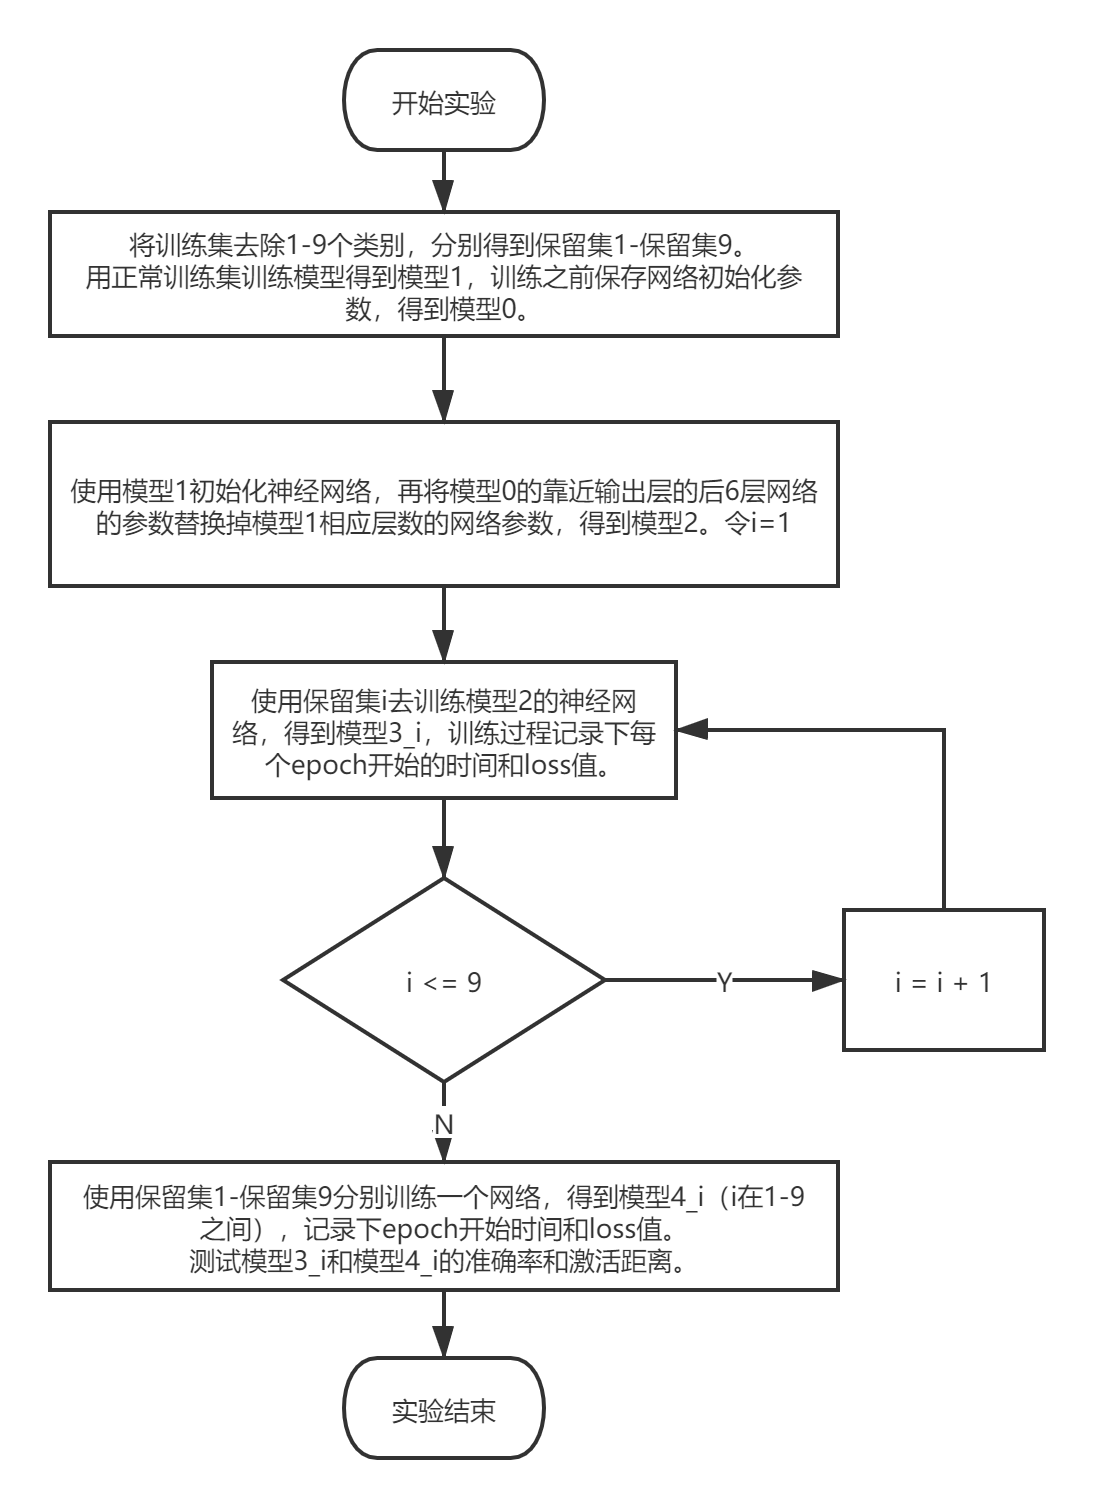
\includegraphics[scale=0.32]{chapter4_process_4.png}
    \caption{遗忘可持续性验证实验流程图}
    \label{fig:chapter4_process_4}
\end{figure}

本实验为了检验冻结重置方法随着遗忘类别数量的增多,其性能是否会发生明显变化。如图\ref{fig:chapter4_process_4}所示,
首先,将训练数据去除一个类别的数据,得到了保留集1;接着将原来完整的训练数据再去掉两个类别的数据便得到了保留集2。以此类推,一共得到9个保留集。这9个保留集均是保留训练集。
用正常训练集训练神经网络得到模型1,在正常训练集训练之前保留网络参数得到模型0。
用神经网络加载模型1,然后把神经网络全连接层和靠近输出层的5层卷积层的参数重置为模型0的相应层次的参数,得到模型2\_1到模型2\_9。
然后分别用保留集1-保留集9去训练模型,训练过程中冻结除了全连接层和后5层卷积层的参数。得到模型3\_1到模型3\_9。
然后使用保留集1-保留集9分别重新训练模型,得到模型4\_1到模型4\_9。
训练过程中记录各Epoch开始时间和损失函数Loss值。
与取得保留训练集类似,我们将测试集去掉一个类别的测试数据便得到保留测试集1,去掉2个类别的测试数据便得到保留测试集2。以此类推,一共得到9个保留测试集。
然后用9个保留测试集分别测试模型3\_1到模型3\_9,还有模型4\_1到模型4\_9的准确率、收敛时间以及激活距离。

\section{实验结果}
\subsection{确定冻结层数实验}
\begin{figure}
    \centering
    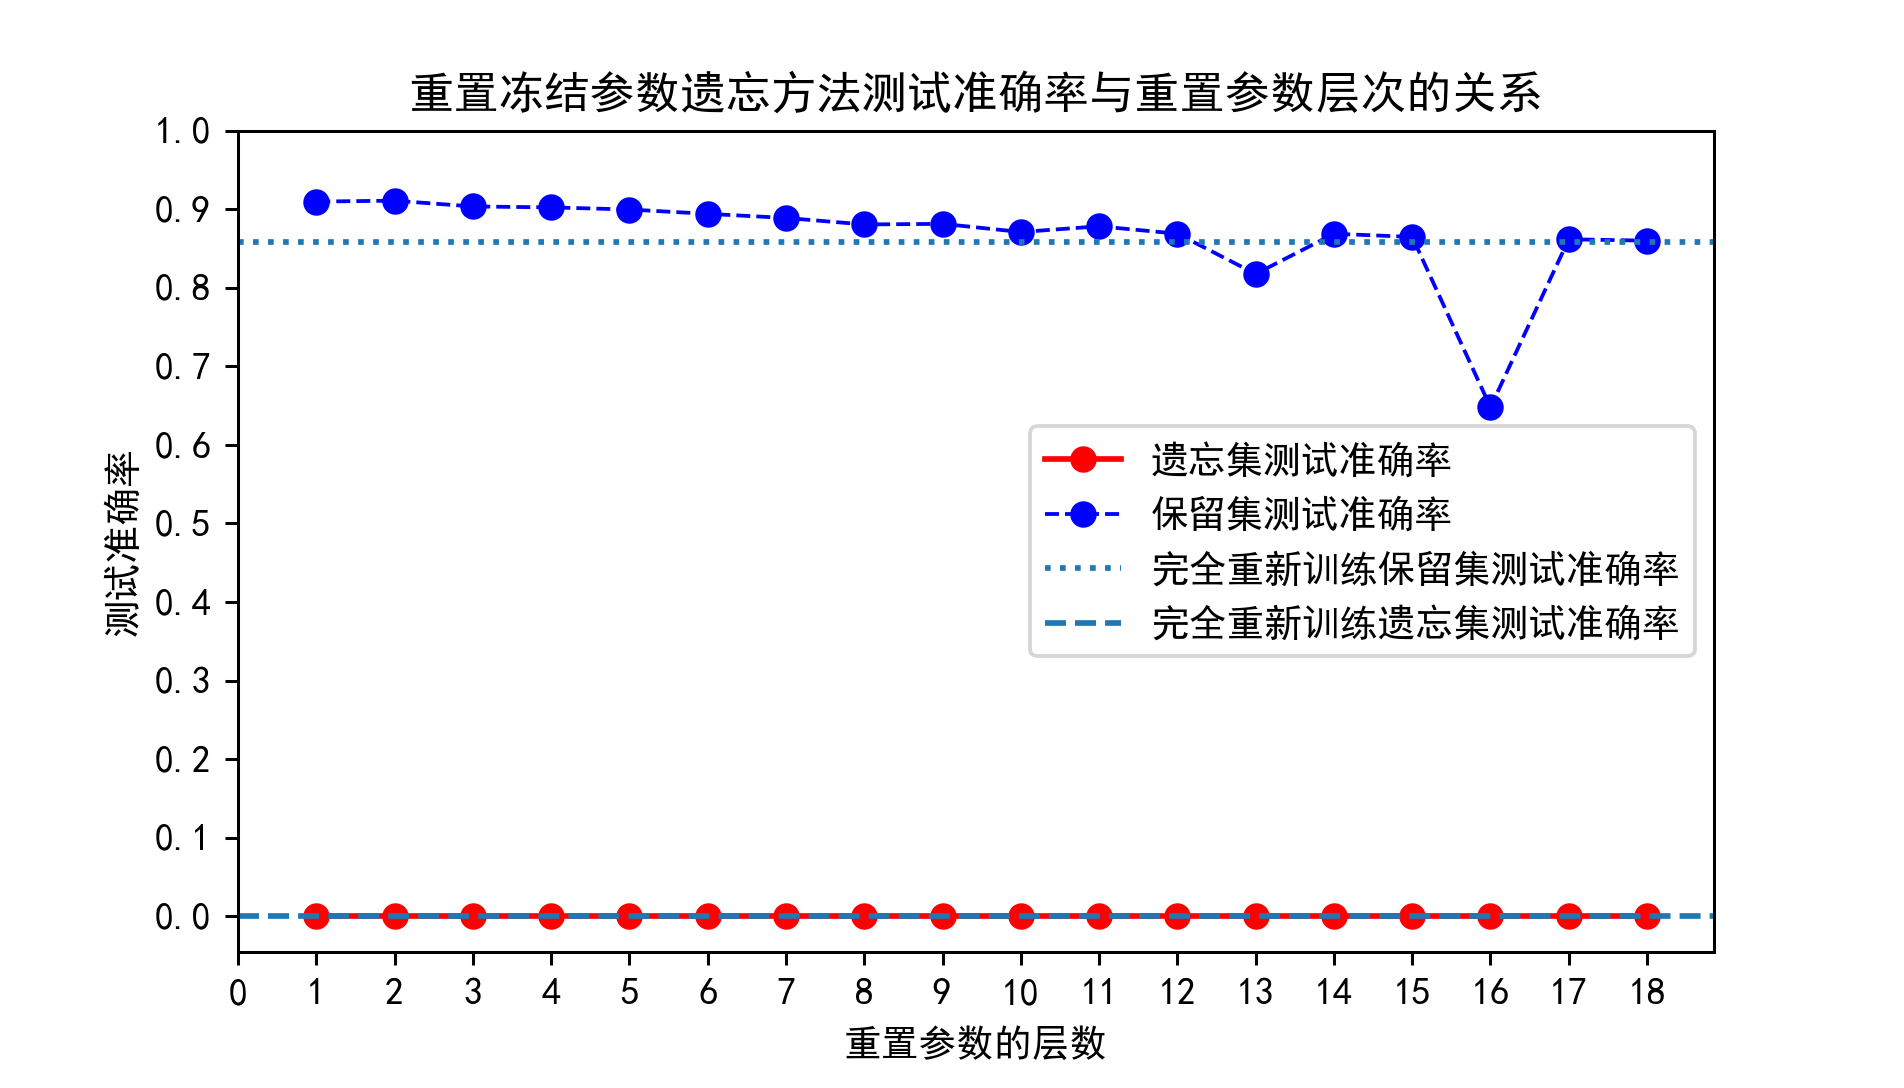
\includegraphics[width=0.9\linewidth]{chapter4_1.png}
    \caption{重置冻结参数遗忘方法测试准确率与重置参数层次的关系}
    \label{fig:chapter4_1}
\end{figure}

如图\ref{fig:chapter4_1}所示,图中展示了本文所讲述的重置冻结参数遗忘方法训练的网络用遗忘测试集和保留测试集测试之后得到准确率。
蓝色的折线代表利用保留测试集测试的准确率,红色的折线代表使用遗忘测试集测试的准确率。
从红线可以看出,遗忘测试集的准确率全是0。这样的结果与完全重新训练得到的模型在遗忘测试集上的准确率完全相同。这说明使用本文提出的冻结重置参数方法,无论重置多少层参数,在遗忘集上均能达到理想的效果。
从蓝线与上面的点线可以看出,本方法得到的模型在保留集测试准确率上在大部分情况下均好于完全重新训练得到的模型在保留集上的准确率。
从蓝色圆点虚线中也发现随着重置参数的层数的增加,其保留集测试准确率有下降趋势,逐渐接近完全重新训练模型在保留集上的测试结果。

\begin{figure}
    \centering
    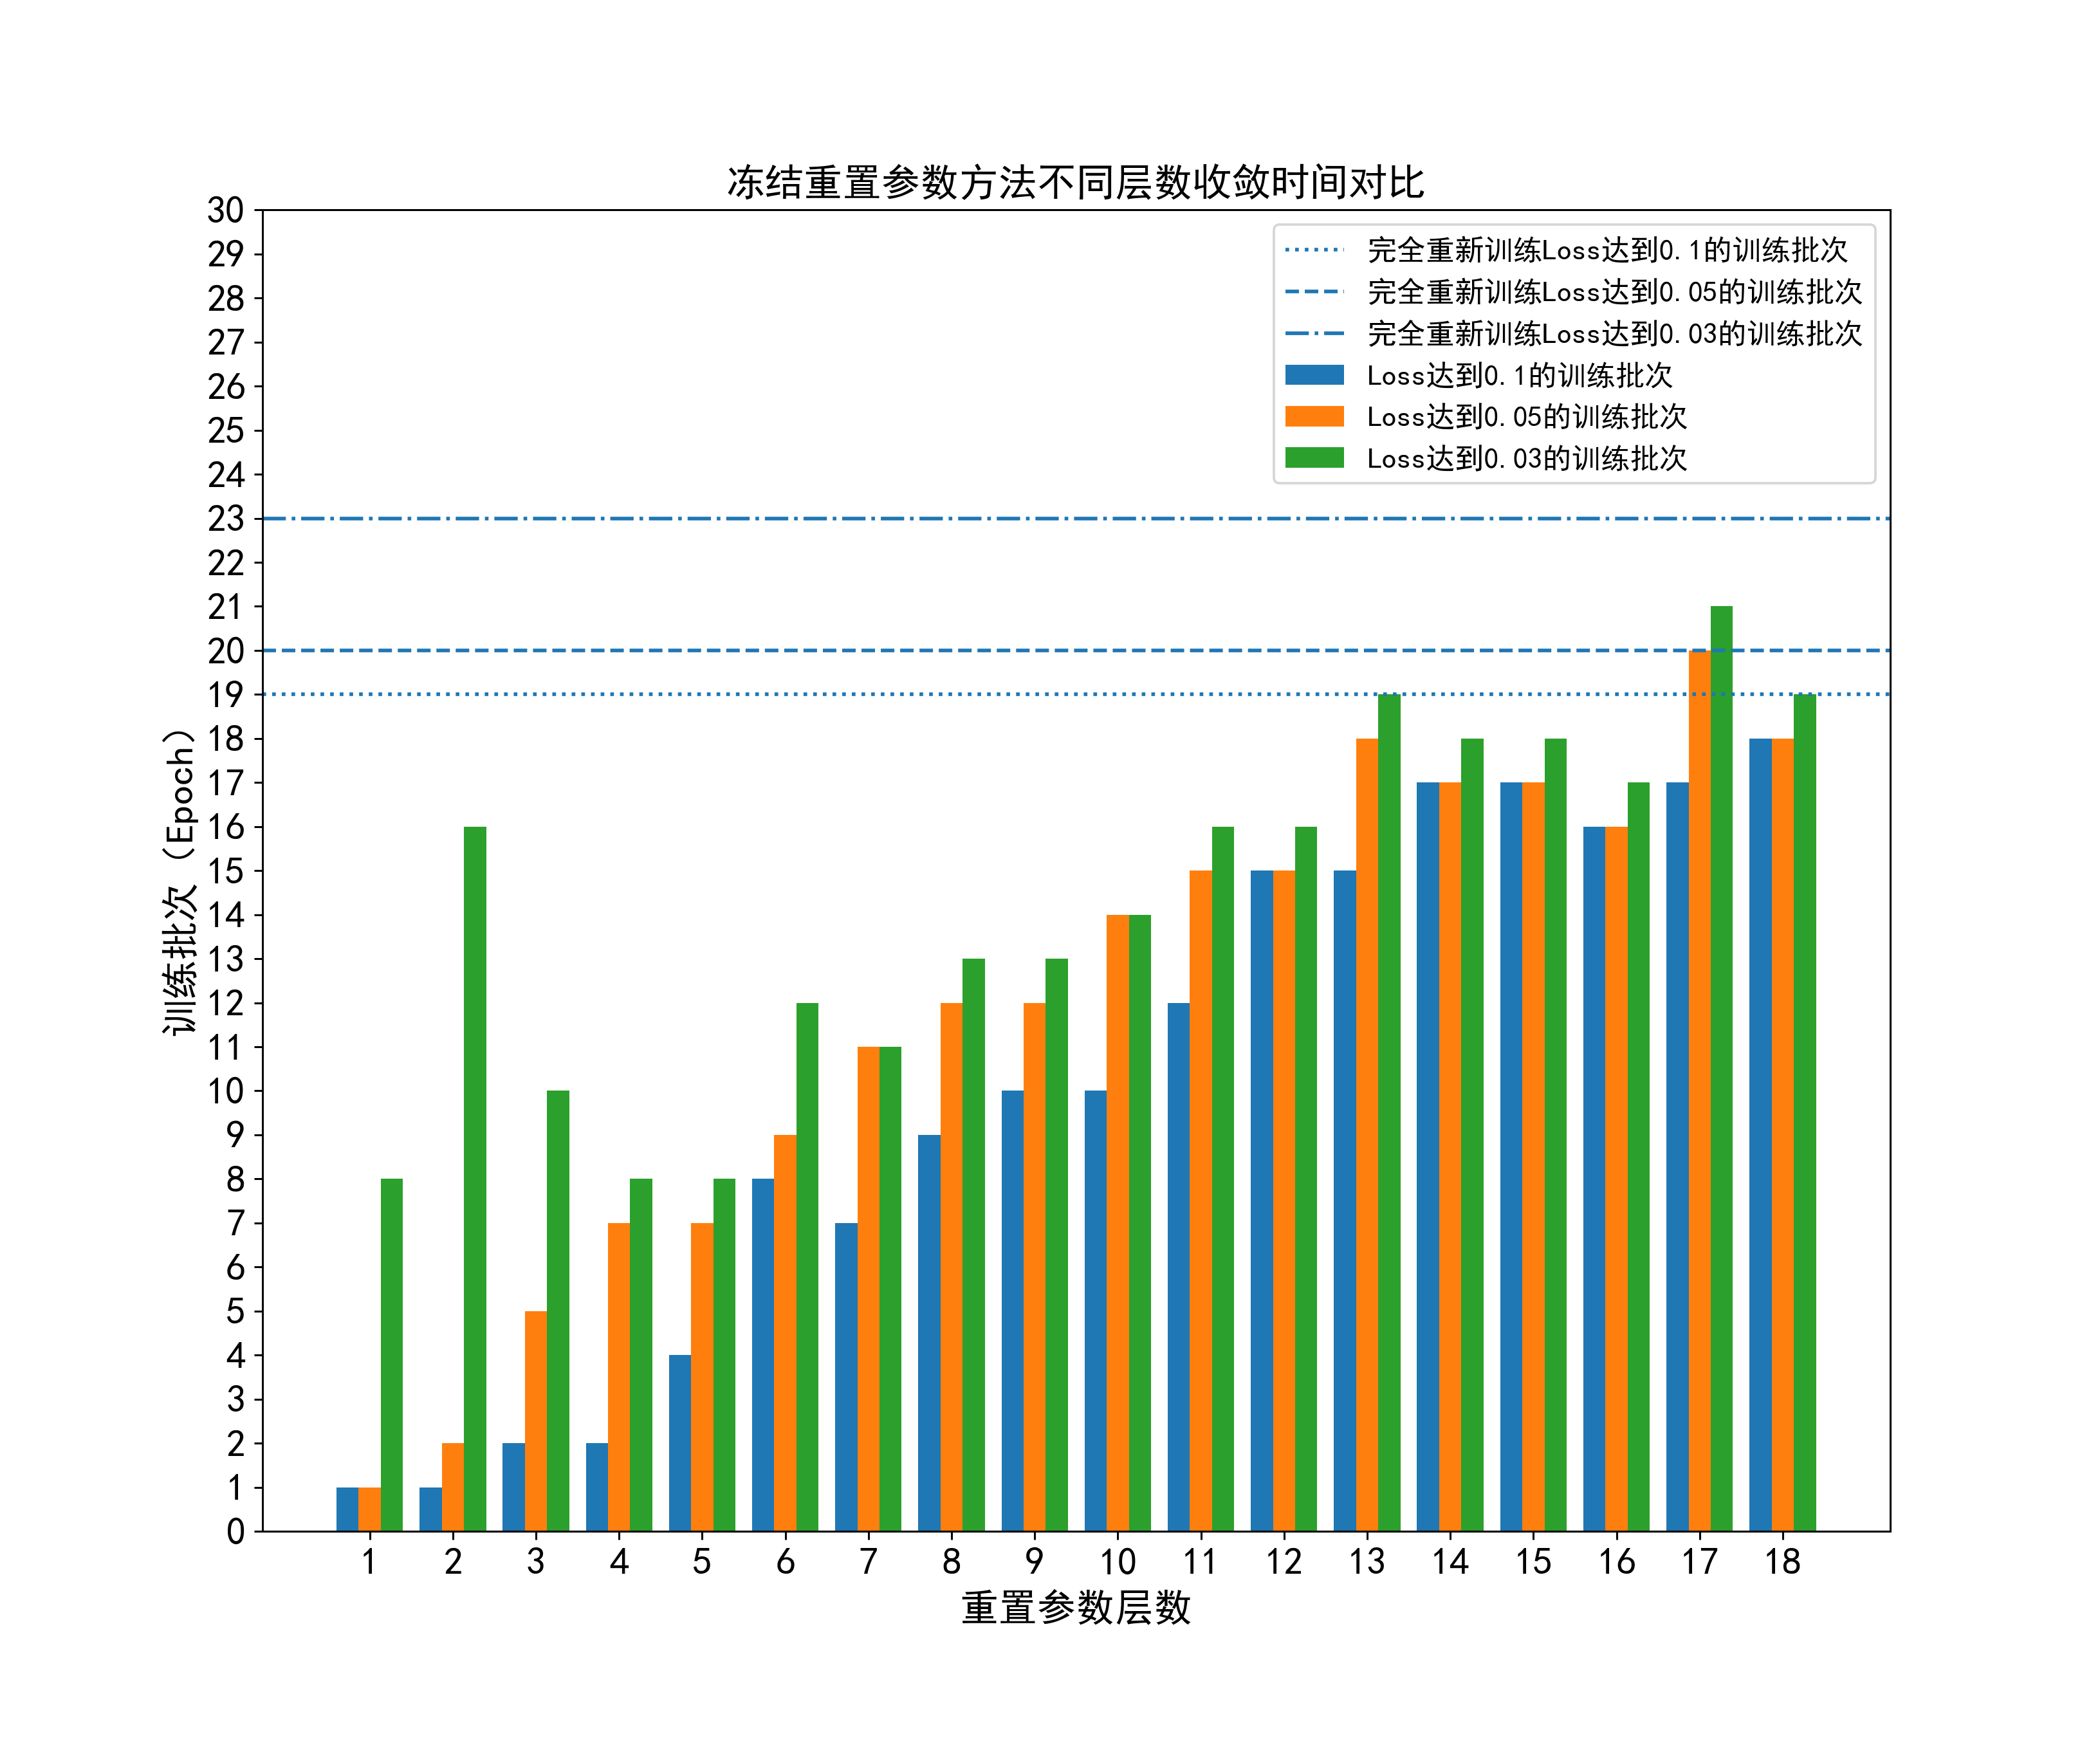
\includegraphics[width=1\linewidth]{chapter4_time_1.png}
    \caption{冻结重置参数方法不同层数收敛时间对比}
    \label{fig:chapter4_time_1}
\end{figure}

如图\ref{fig:chapter4_time_1}所示,图中展示了本文所讲述的重置冻结参数遗忘方法在重置不同层次参数上使用保留集训练后收敛时间的对比。
图中展示了三套柱图的对比,蓝色柱图、黄色柱图和绿色柱图分别代表使用保留训练集训练网络时,该训练批次(Epoch)的平均损失函数Loss的值首次降到0.1,0.05和0.03以下时的训练批次(Epoch)数。
批次数越小,说明训练的收敛时间越快。上面有三条不同线型的横线,分别代表完全重新训练网络时,该训练过程的平均损失函数值首次降到0.1,0.05和0.03以下时的训练批次(Epoch)数。
这三条横线的作用是与本文提到的方法进行收敛时间上的对比。
从图中的柱状图可以看出,随着重置参数的层数逐渐增多,其收敛的Epoch逐渐增大,逐渐接近完全重新训练时收敛的Epoch。
其实这也不难理解,随着重置参数的层数增多,网络中需要更新的参数也逐渐增多,其状态也越来越接近完全重新训练的情况,所以收敛时间也逐步接近完全重新训练。
我们希望选择的层次是选择该层次后,训练后的准确率越高越好,训练收敛时间越快越好。
所以综合图\ref{fig:chapter4_1}和\ref{fig:chapter4_time_1},可以备选的层次是前7层均在可以接受的范围内,重置参数层数越小,准确率越高,收敛时间也越快。
\begin{figure}
    \centering
    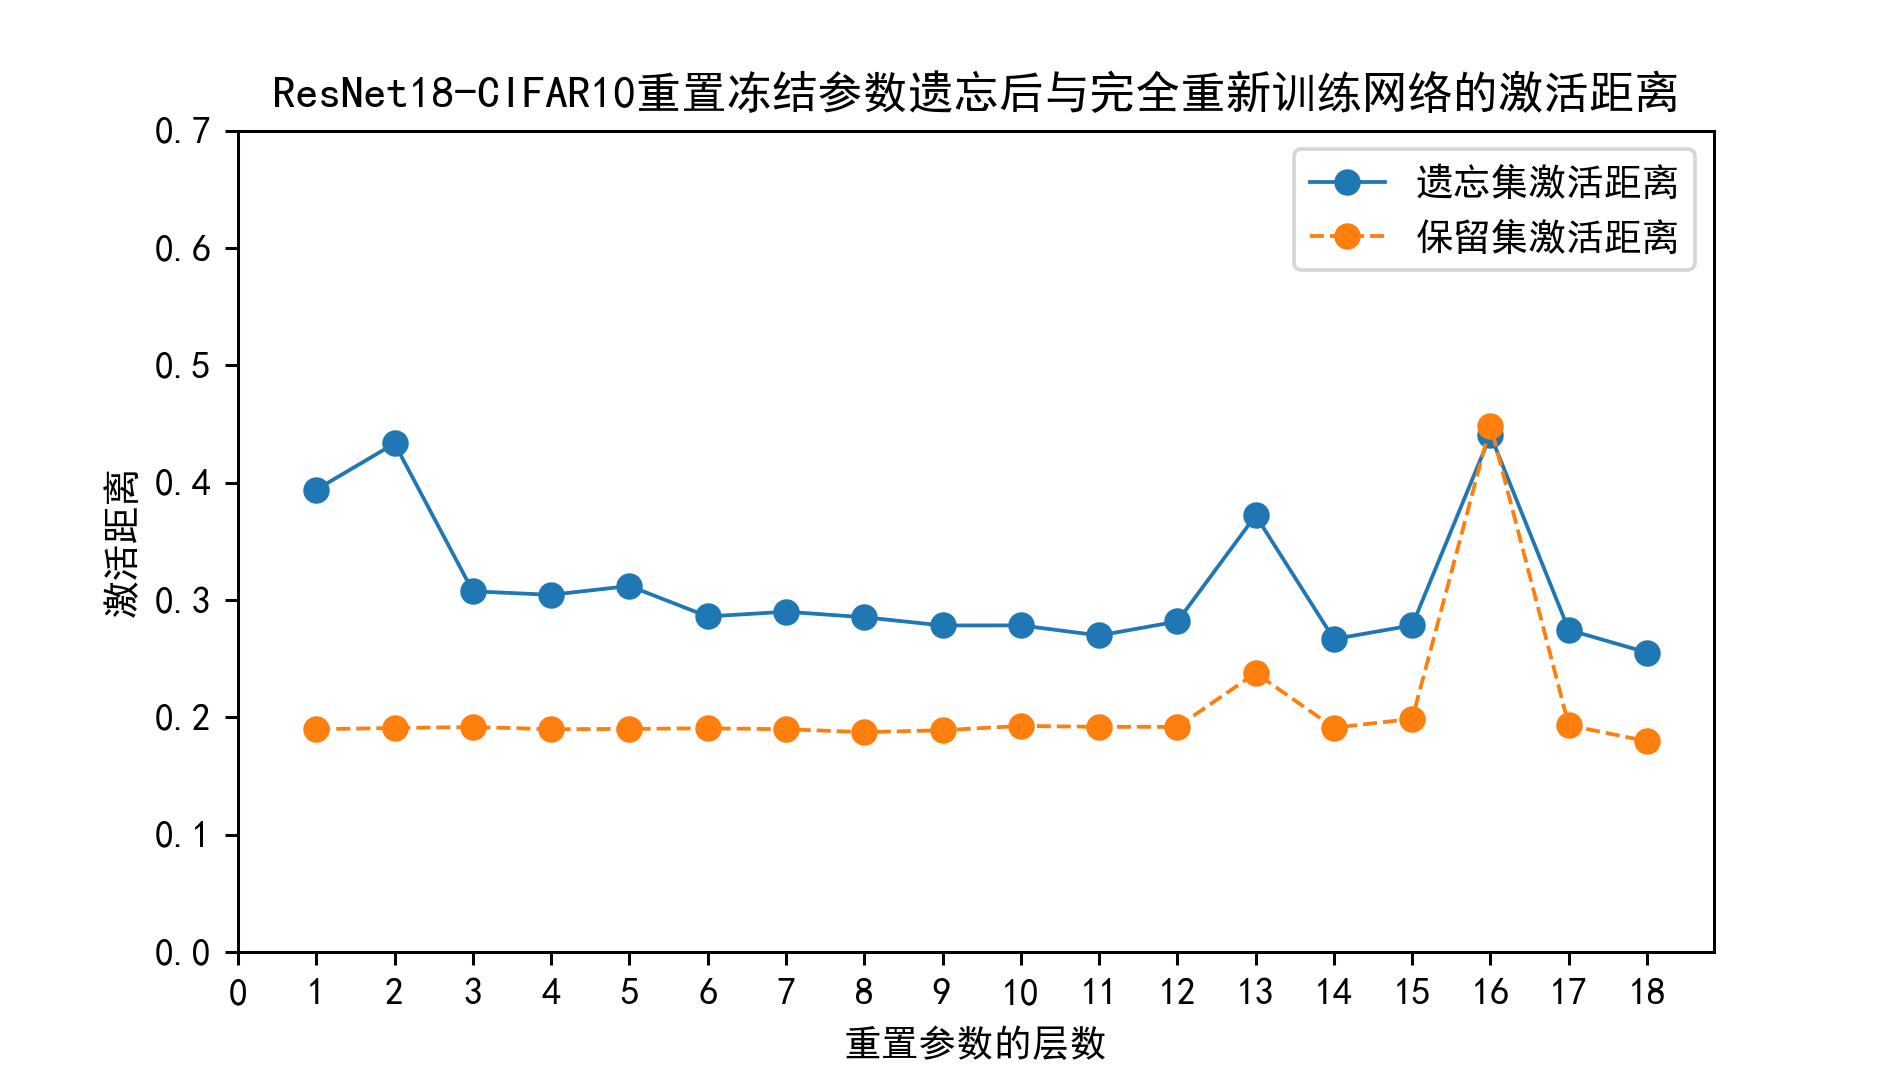
\includegraphics[width=0.9\linewidth]{chapter4_distance_1.png}
    \caption{重置冻结参数遗忘后与完全重新训练网络的激活距离}
    \label{fig:chapter4_distance_1}
\end{figure}

如图\ref{fig:chapter4_distance_1}所示,图中展示了本文所讲述的重置冻结参数遗忘方法训练的网络与完全重新训练的网络之间对于测试集输出之间的激活距离。
激活距离在上一节有具体讲到,是两个网络输出向量差的绝对值的第二范数值在测试数据集上的期望。
蓝色折线代表两个网络在遗忘测试集上的激活距离,橙色折线代表两个网络在保留集上的激活距离。从图中可以看出,两个网络在遗忘测试集上的激活距离要高于在保留测试集上的激活距离。
我们对于两个网络激活距离的期望是越小越好,在前7层可以看到保留测试集的激活距离普遍稳定地保持较低数值,而对于遗忘测试集的激活距离前2层的数值相对较大,3、4、5层数值也略大,从第6层开始,数值变得平稳。
因此,综合图\ref{fig:chapter4_1}和图\ref{fig:chapter4_time_1}和图\ref{fig:chapter4_distance_1}的分析结果,我们选择第6层作为重置冻结参数遗忘方法对于ResNet18网络重置参数的层数。
\subsection{冻结必要性验证实验}
\begin{figure}
    \centering
    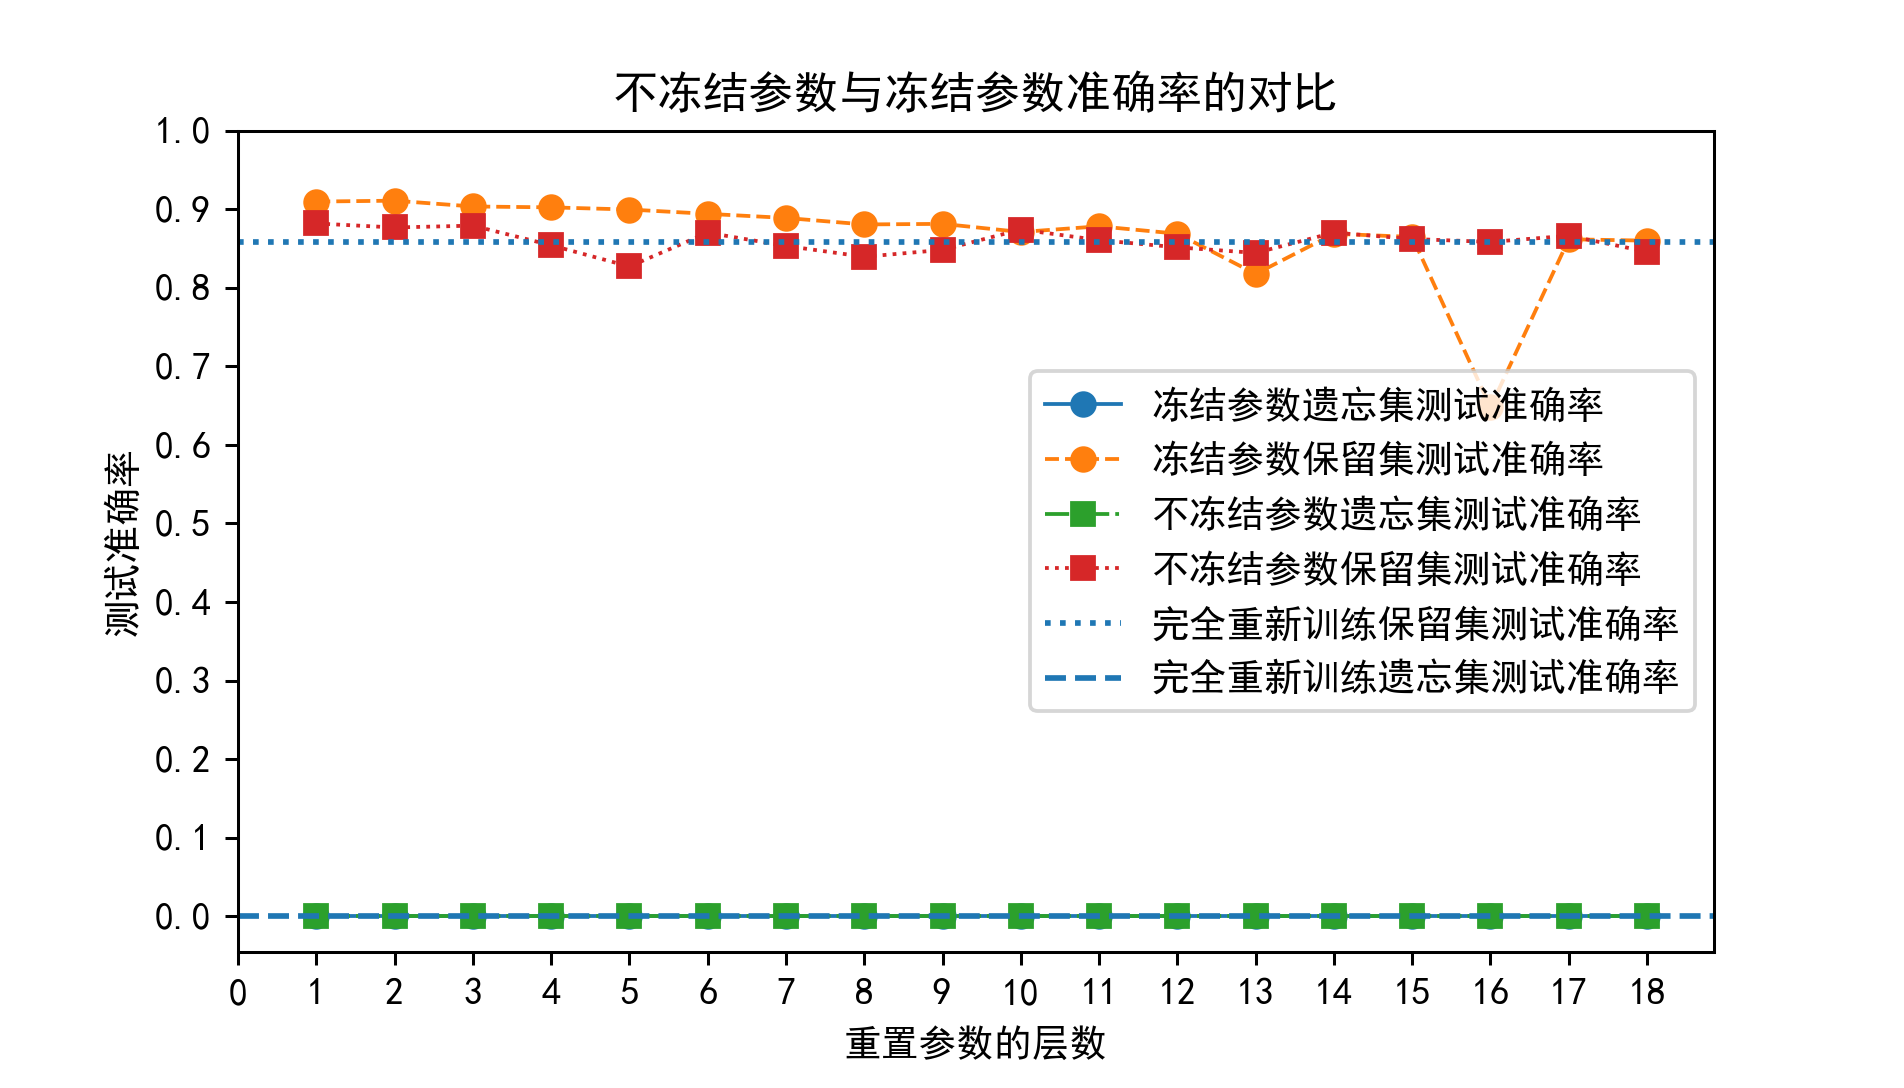
\includegraphics[width=0.9\linewidth]{chapter4_2.png}
    \caption{不冻结参数与冻结参数准确率的对比}
    \label{fig:chapter4_2}
\end{figure}

如图\ref{fig:chapter4_2}所示,图中展示了重置一定参数后冻结参数与不冻结参数训练对遗忘类别和保留类别准确率的影响。
橘黄色圆点折线代表冻结参数情况下网络在保留测试集上的准确率,蓝色圆点折线代表该网络在遗忘测试集上得到的准确率。
红色方格折线代表不冻结参数的情况下在保留测试集上的准确率,绿色方格折线代表该网络在遗忘测试集上得到的准确率。
除此之外,图中还画了两条横线,点线代表完全重新训练的网络模型在保留测试集上得到的准确率,虚线代表完全重新训练的网络模型在遗忘测试集上得到的准确率。
这两条横线的主要作用是作为冻结参数和不冻结参数准确率的参照。通过橘黄色圆点折线和红色方格折线可以看出冻结参数与不冻结参数在保留测试集的准确率上总体相差不大,但是冻结参数的方法要略好于不冻结参数方法。
在遗忘测试集的准确率上,两种方法效果相同,均为0。
\begin{figure}
    \centering
    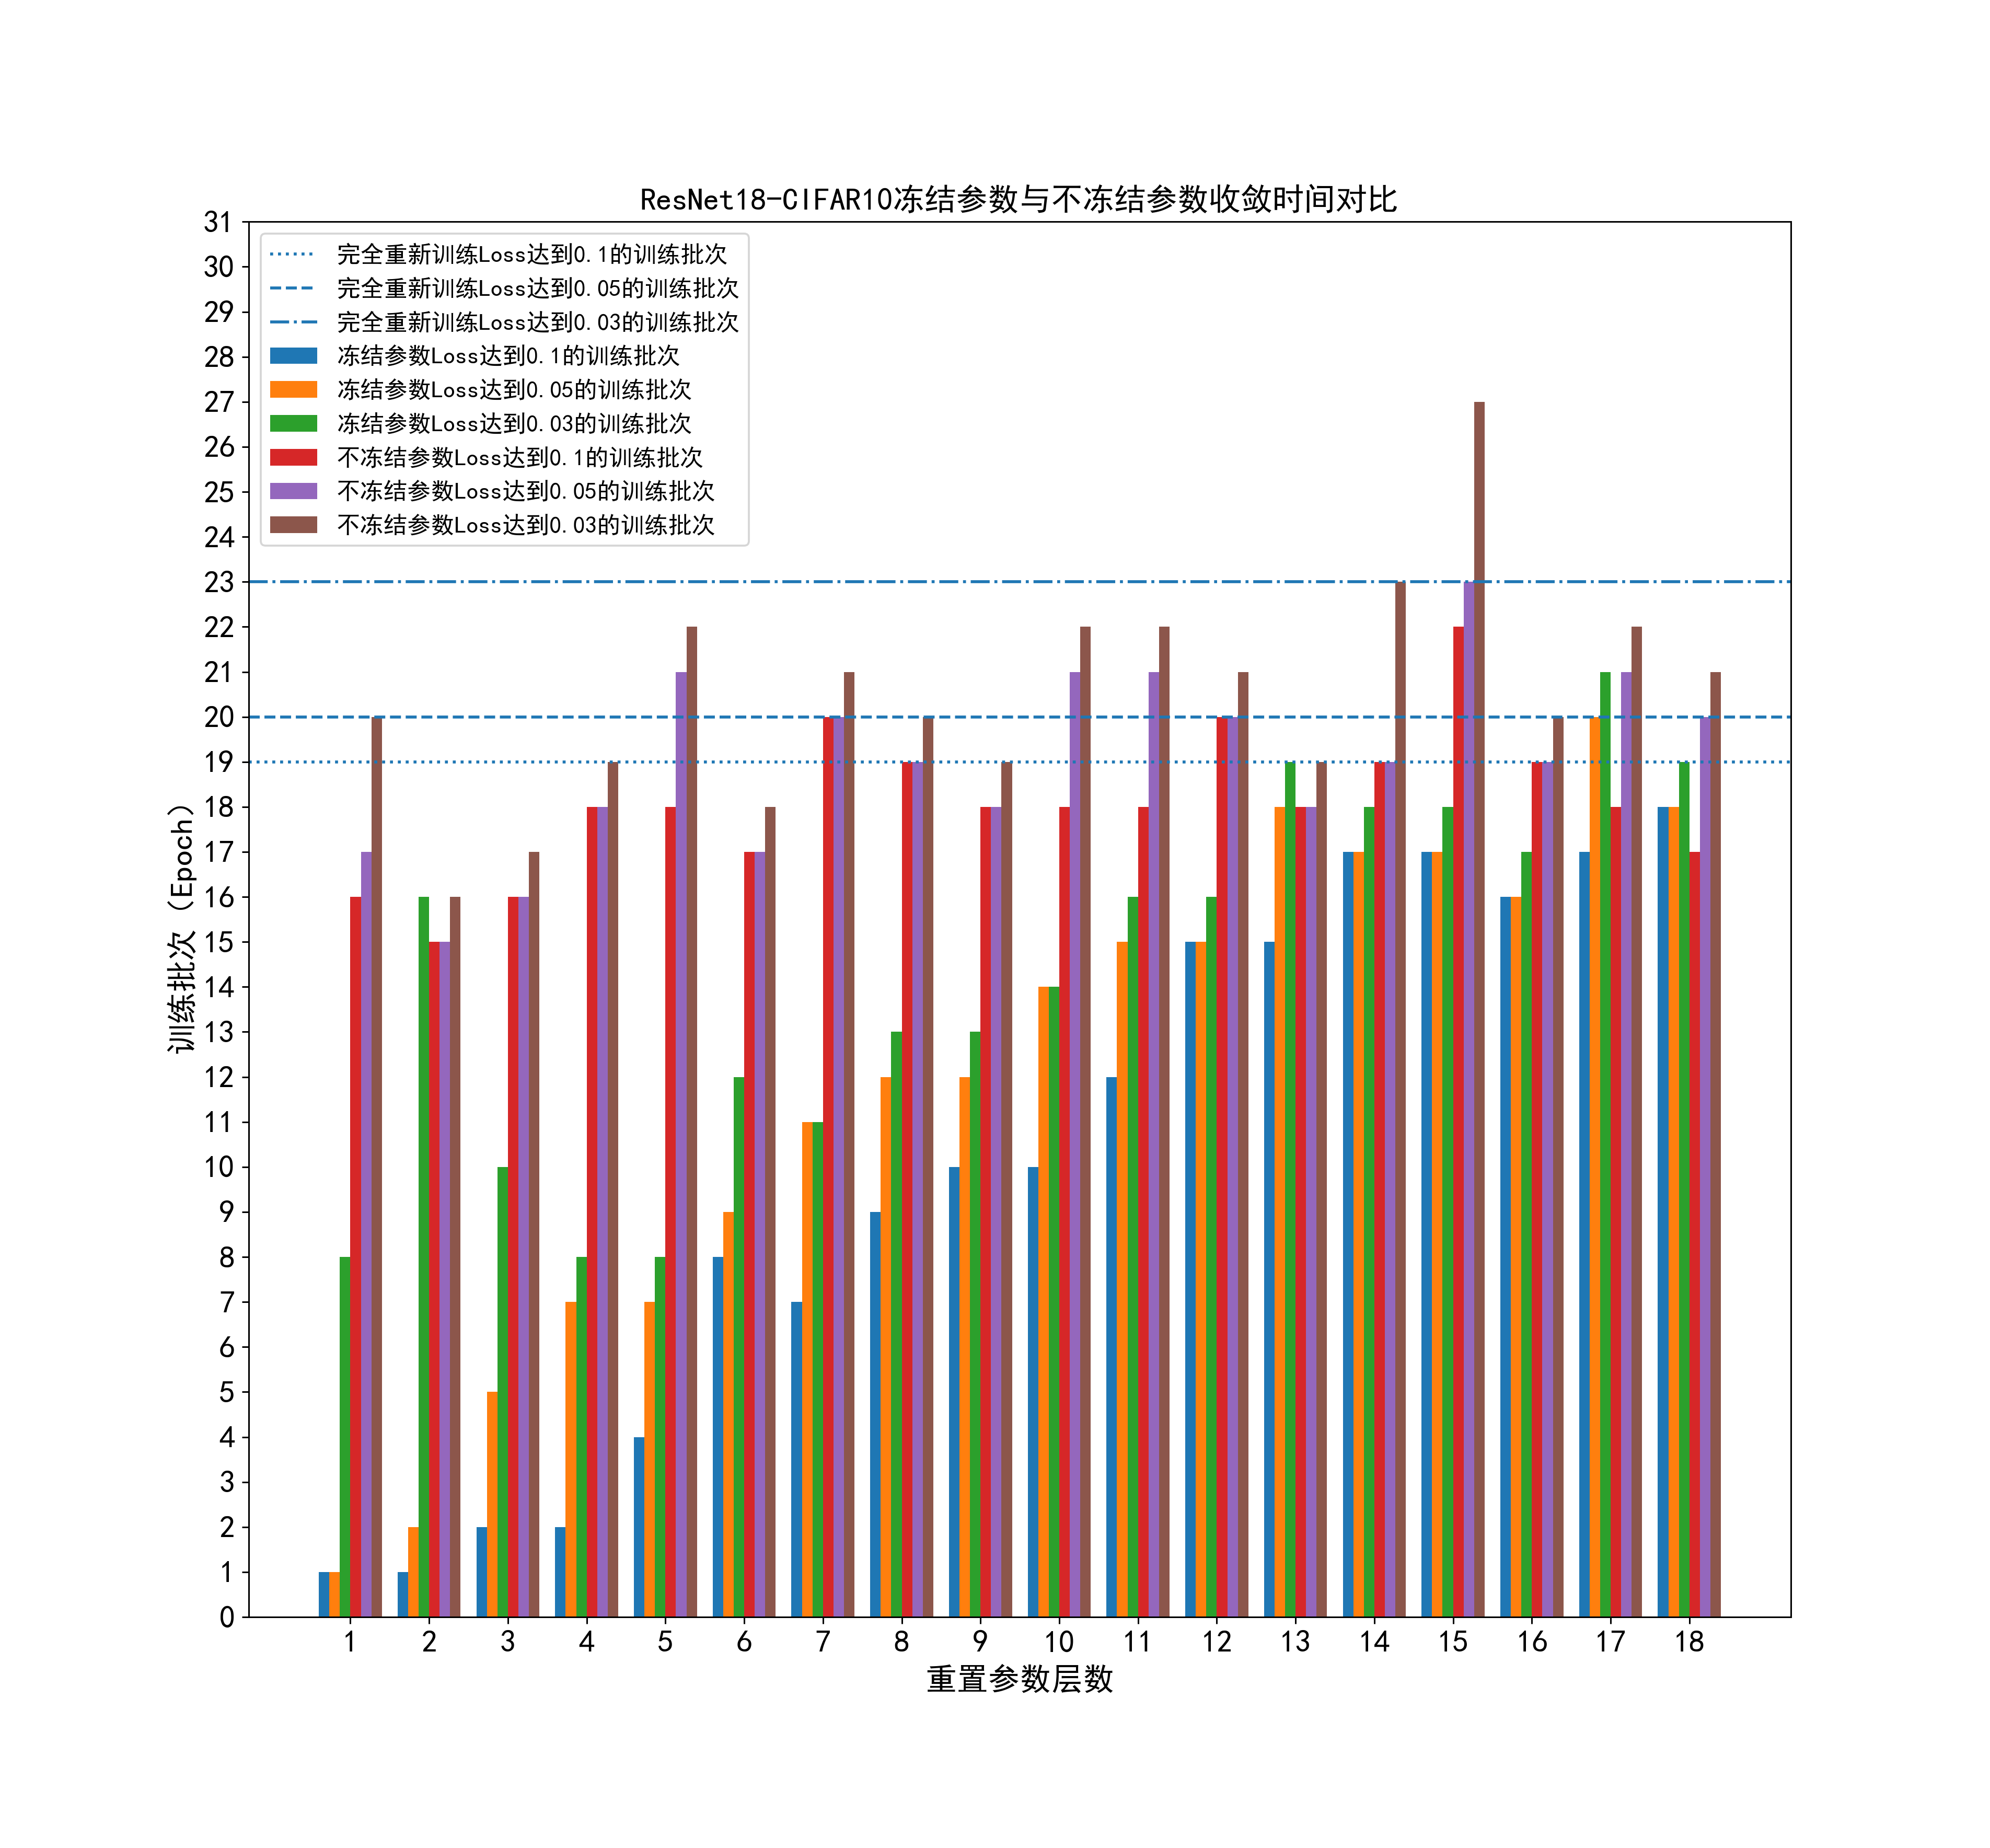
\includegraphics[width=1\linewidth]{chapter4_time_2.png}
    \caption{冻结参数与不冻结参数收敛时间对比}
    \label{fig:chapter4_time_2}
\end{figure}

如图\ref{fig:chapter4_time_2}所示,图中展示了冻结参数与不冻结参数重置参数后使用保留训练集训练网络的收敛时间。
蓝色、黄色和绿色柱图分别代表冻结参数情况下网络的平均损失函数值收敛到0.1、0.05和0.03时所花费的训练周期,即Epoch数。
粉色、紫色和棕色柱图分别代表非冻结参数情况下网络的平均损失函数收敛到0.1、0.05和0.03时所花费的训练周期数。
上面画出的三条横线,点线、虚线和点划线分别代表完全重新训练网络过程中,网络的平均损失函数值收敛至0.1、0.05和0.03时所花费的训练周期数。其主要作用是用来提供参照。
通过观察冻结参数和不冻结参数的柱状图可以发现,冻结参数后训练的收敛时间从整体上要少于不冻结参数训练网络收敛时间。这个现象也是符合逻辑的。
冻结参数后,一部分参数不需要计算更新,而没有冻结参数的网络则需要计算所有参数的更新。所以从计算量上分析,不冻结参数训练网络所需要的工作量是比冻结参数要大的。
通过图\ref{fig:chapter4_2}和图\ref{fig:chapter4_time_2}的结果可以初步得出结论,冻结参数训练网络的方法要好于不冻结参数训练网络的方法。
\begin{figure}
    \centering
    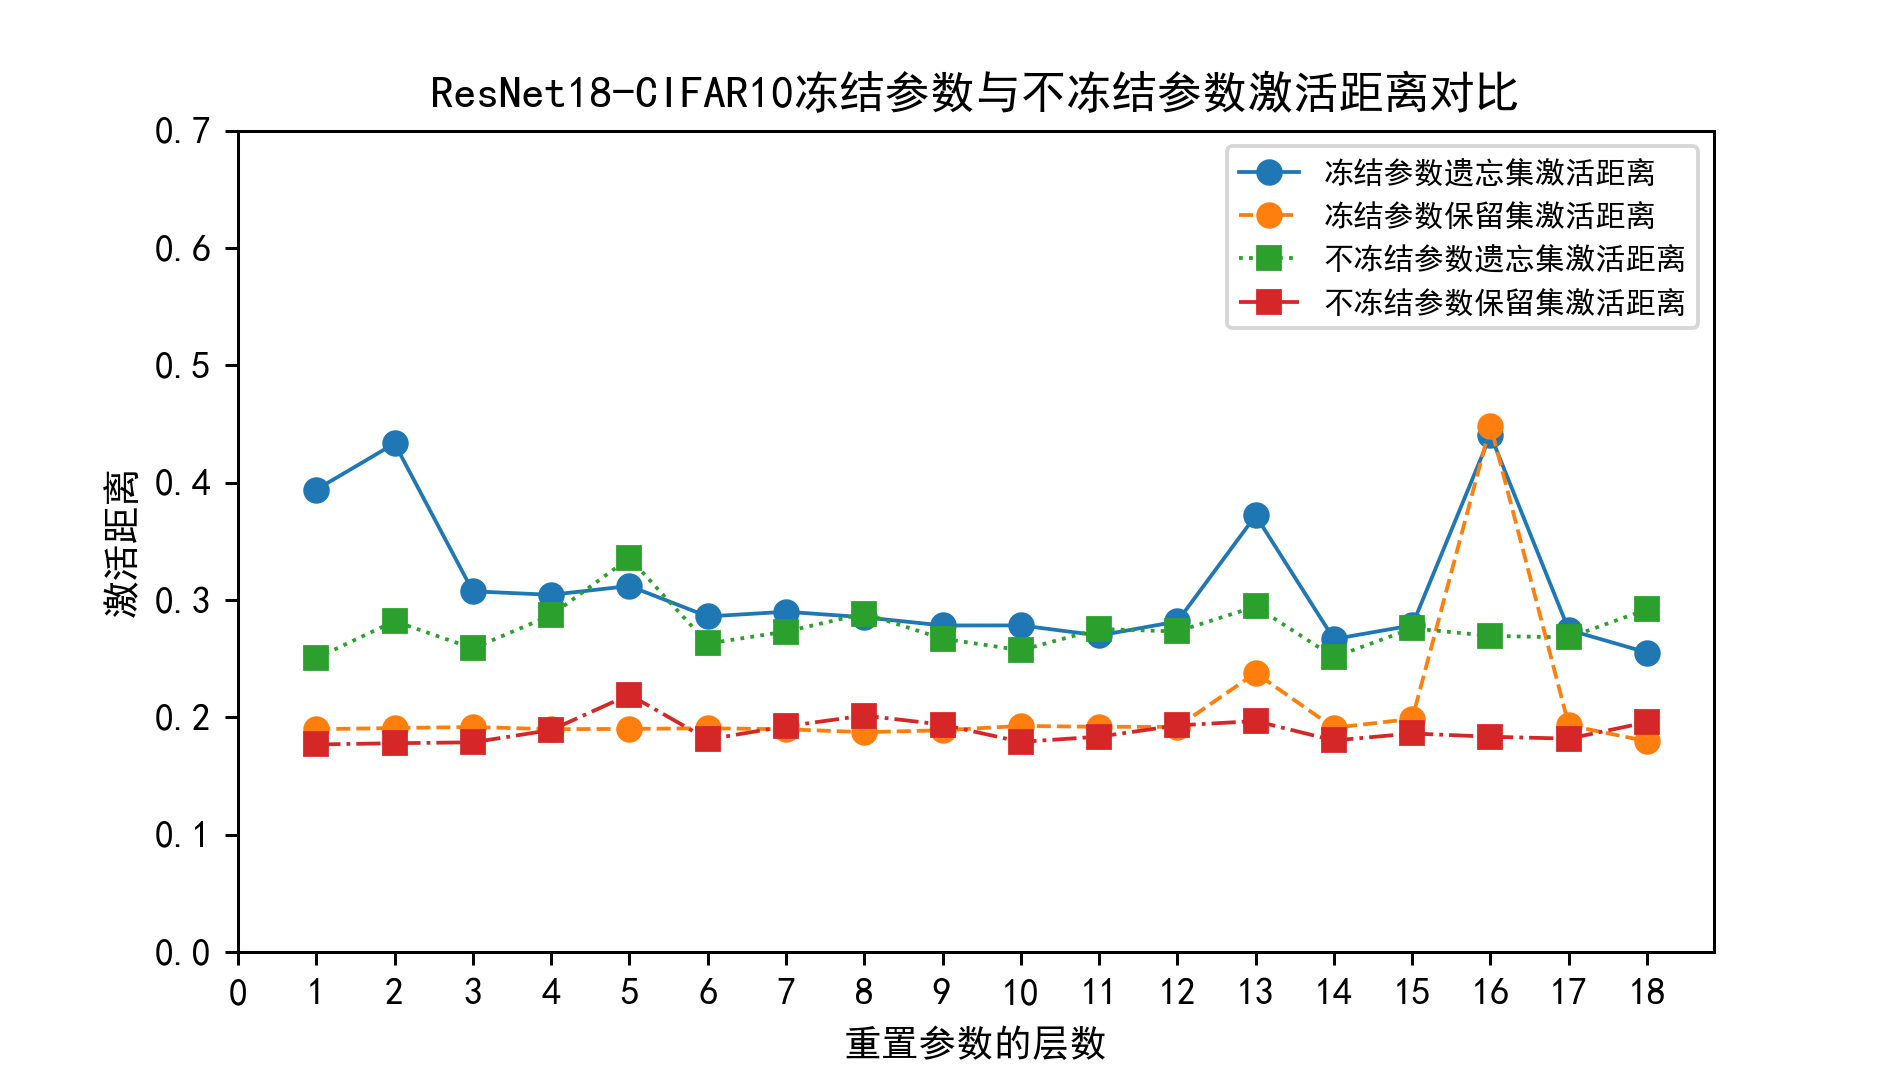
\includegraphics[width=0.9\linewidth]{chapter4_distance_2.png}
    \caption{冻结参数与不冻结参数激活距离对比}
    \label{fig:chapter4_distance_2}
\end{figure}

如图\ref{fig:chapter4_distance_2}所示,图中展示了冻结参数与不冻结参数的两个网络在激活距离上的对比。这两个网络参照的对象均是完全重新训练生成的网络。
蓝色圆点折线和黄色圆点折线分别代表冻结参数的情况下,分别使用遗忘测试集和保留测试集测试网络,两个网络的输出与重新训练网络的输出距离。
同样,绿色方块折线和红色方块折线分别代表在不冻结参数情况下分别用遗忘测试集和保留测试集进行测试,两个网络的输出与重新训练网络输出的距离。
从图中可以看出,冻结参数的方法和不冻结参数的方法,在保留测试集上的激活距离相差无几,并且从整体水平上低于在遗忘测试集上产生的激活距离。
在用遗忘测试集测试的网络输出距离上,冻结参数的方法在前三层时激活距离比不冻结参数的要大,可是从第三层往后的层次冻结与不冻结的激活距离很相近。因此重置参数的层数选择第三层以后,这个差异是可以忽略不计的。

\subsection{反向冻结验证实验}
\begin{figure}
    \centering
    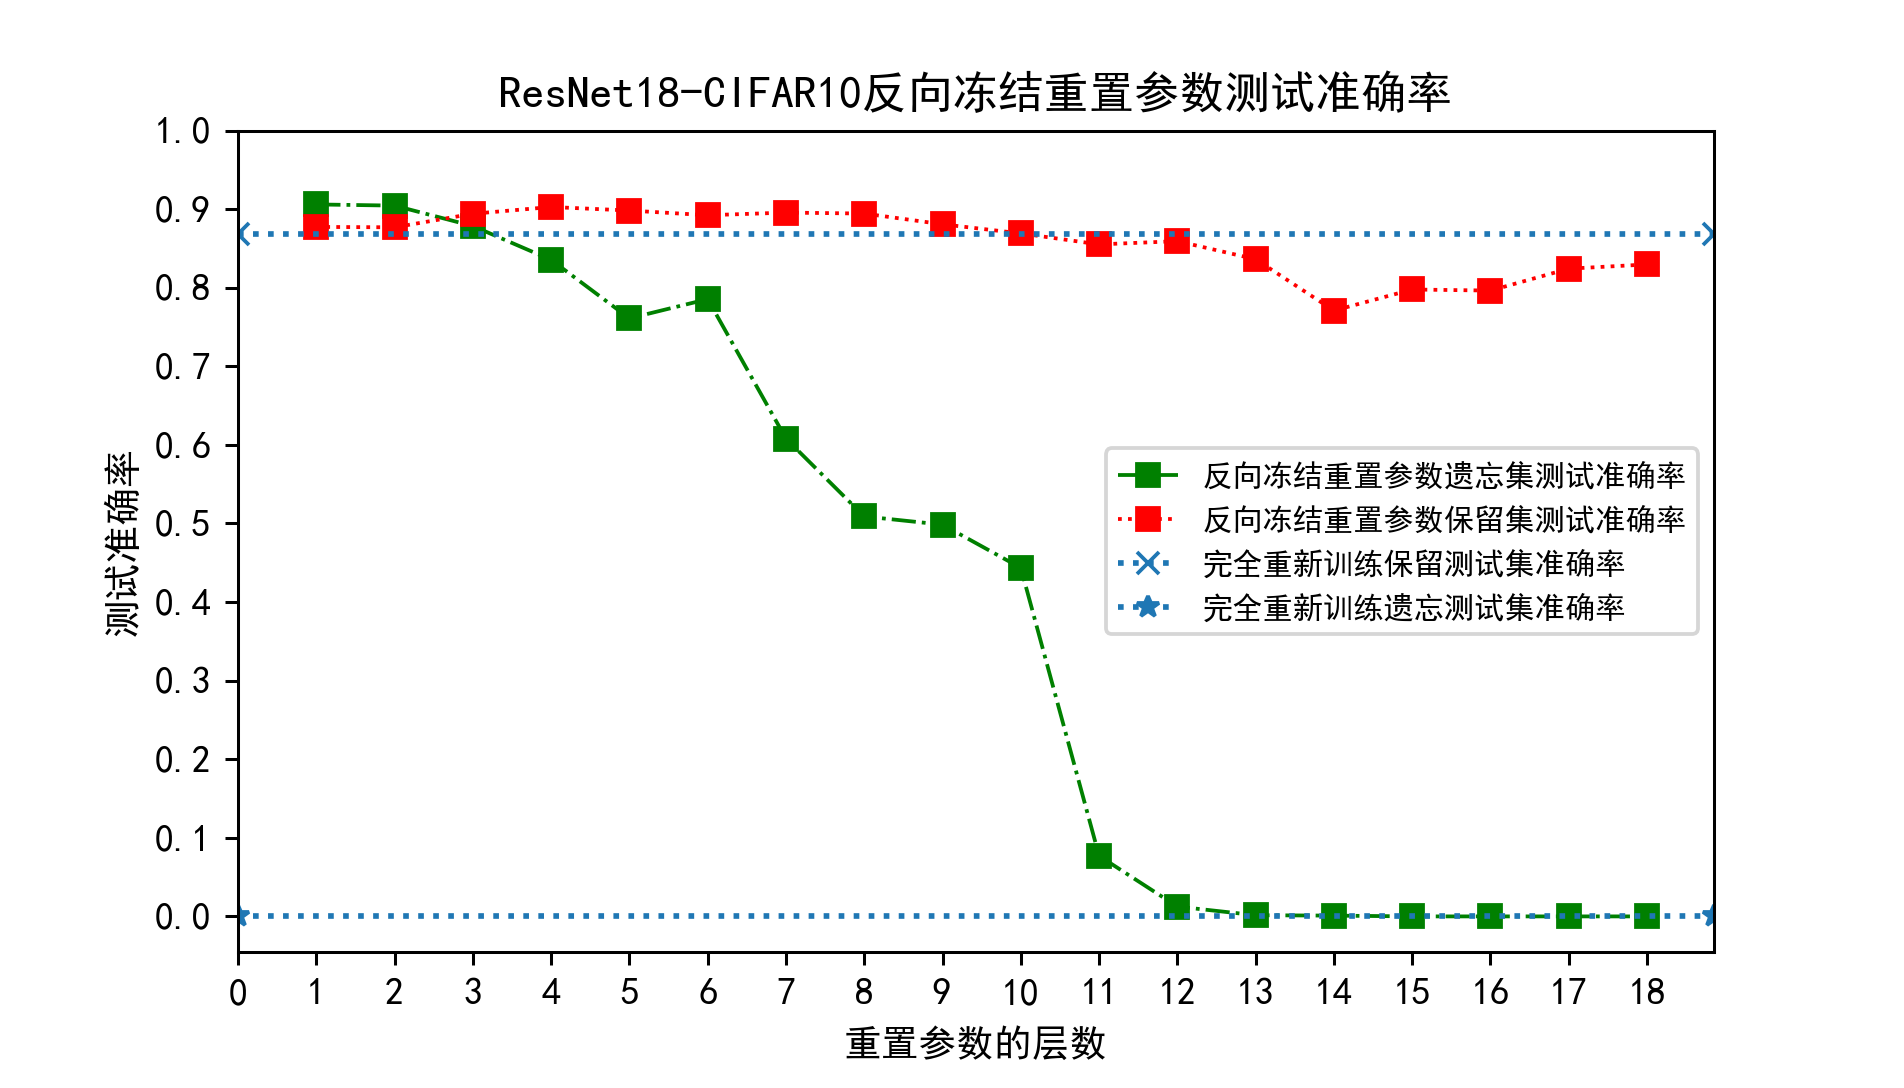
\includegraphics[width=0.9\linewidth]{chapter4_3.png}
    \caption{反向冻结重置参数与正向冻结重置参数测试准确率对比}
    \label{fig:chapter4_3}
\end{figure}

如图\ref{fig:chapter4_3}所示,图中展示了正向冻结参数与反向冻结参数训练后测试准确率的对比。
蓝色圆点和黄色圆点折线分别代表正向冻结参数时遗忘测试集和保留测试集上准确率的数据。绿色方块和红色方块折线分别代表反向冻结参数时遗忘测试集和保留测试集的准确率数据。
为了进行对比,图中还加了两条横线,点线代表完全重新训练网络在保留测试集上的测试结果,虚线代表完全重新训练网络在遗忘测试集上的准确率数据。
从图中可以看出,经过反向冻结后,保留测试集的准确率和正向冻结参数的准确率十分相近。图中,反向冻结与正向冻结最大的不同是蓝色圆点折线和绿色方块折线,他们都是在遗忘测试集下的准确率。
使用正向重置参数方法在遗忘测试集的准确率一直为0,而使用反向冻结参数方法在遗忘测试集上的准确率却是逐步在减少的。在前12层重置参数后利用保留训练集进行训练,遗忘测试集的准确率不为0。
这说明,重置前12层参数时并没有把遗忘类别很好地遗忘掉,有一些通过重置参数而丢失的信息可以通过保留训练集的学习补充回去。

如果将卷积神经网络看成一半是特征提取器,另一半是分类器。这张图很好地说明了哪里是特征提取器和分类器的分界线,就是第13层,倒数第6层。
如绿色方块折线所展示的,在第13层以前,遗忘类别的分类器总能通过保留训练集学到的特征而产生一定的准确率。直到参数重置到了第13层,遗忘类别的分类器无法通过保留训练集学习到的特征而对遗忘集进行准确分类。
这就说明从第一层到第13层均有一定程度的特征提取的作用。从第13层以后,主要作用是用作分类器。我们为了彻底遗忘某个类别,我们应当是重置特征提取器的参数还是分类器的参数呢?
在这里作者认为应当更新分类器的参数。举一个例子,人类都有眼睛、鼻子和耳朵,可是影响一个人识别另一个人的因素往往不是看这个人有没有鼻子,有没有眼睛,因为人人都有鼻子和眼睛。一个人区分不同人靠的是眼睛和鼻子的大小以及眼睛和鼻子等其他器官之间的距离信息。
在卷积神经网络中也是一样,低层的参数就好像在提取最基本的特征,高层的参数去提取这些基本特征之间的位置关系。所以最终影响分类的不是有没有基本特征,而是这些基本特征之间的搭配关系。
在本图中,前12层的参数被更新后,通过学习保留训练集,仍然能学习到遗忘训练集分类所用到的基本特征,所以后6层才是影响遗忘类别分类的主要参数。
\begin{figure}
    \centering
    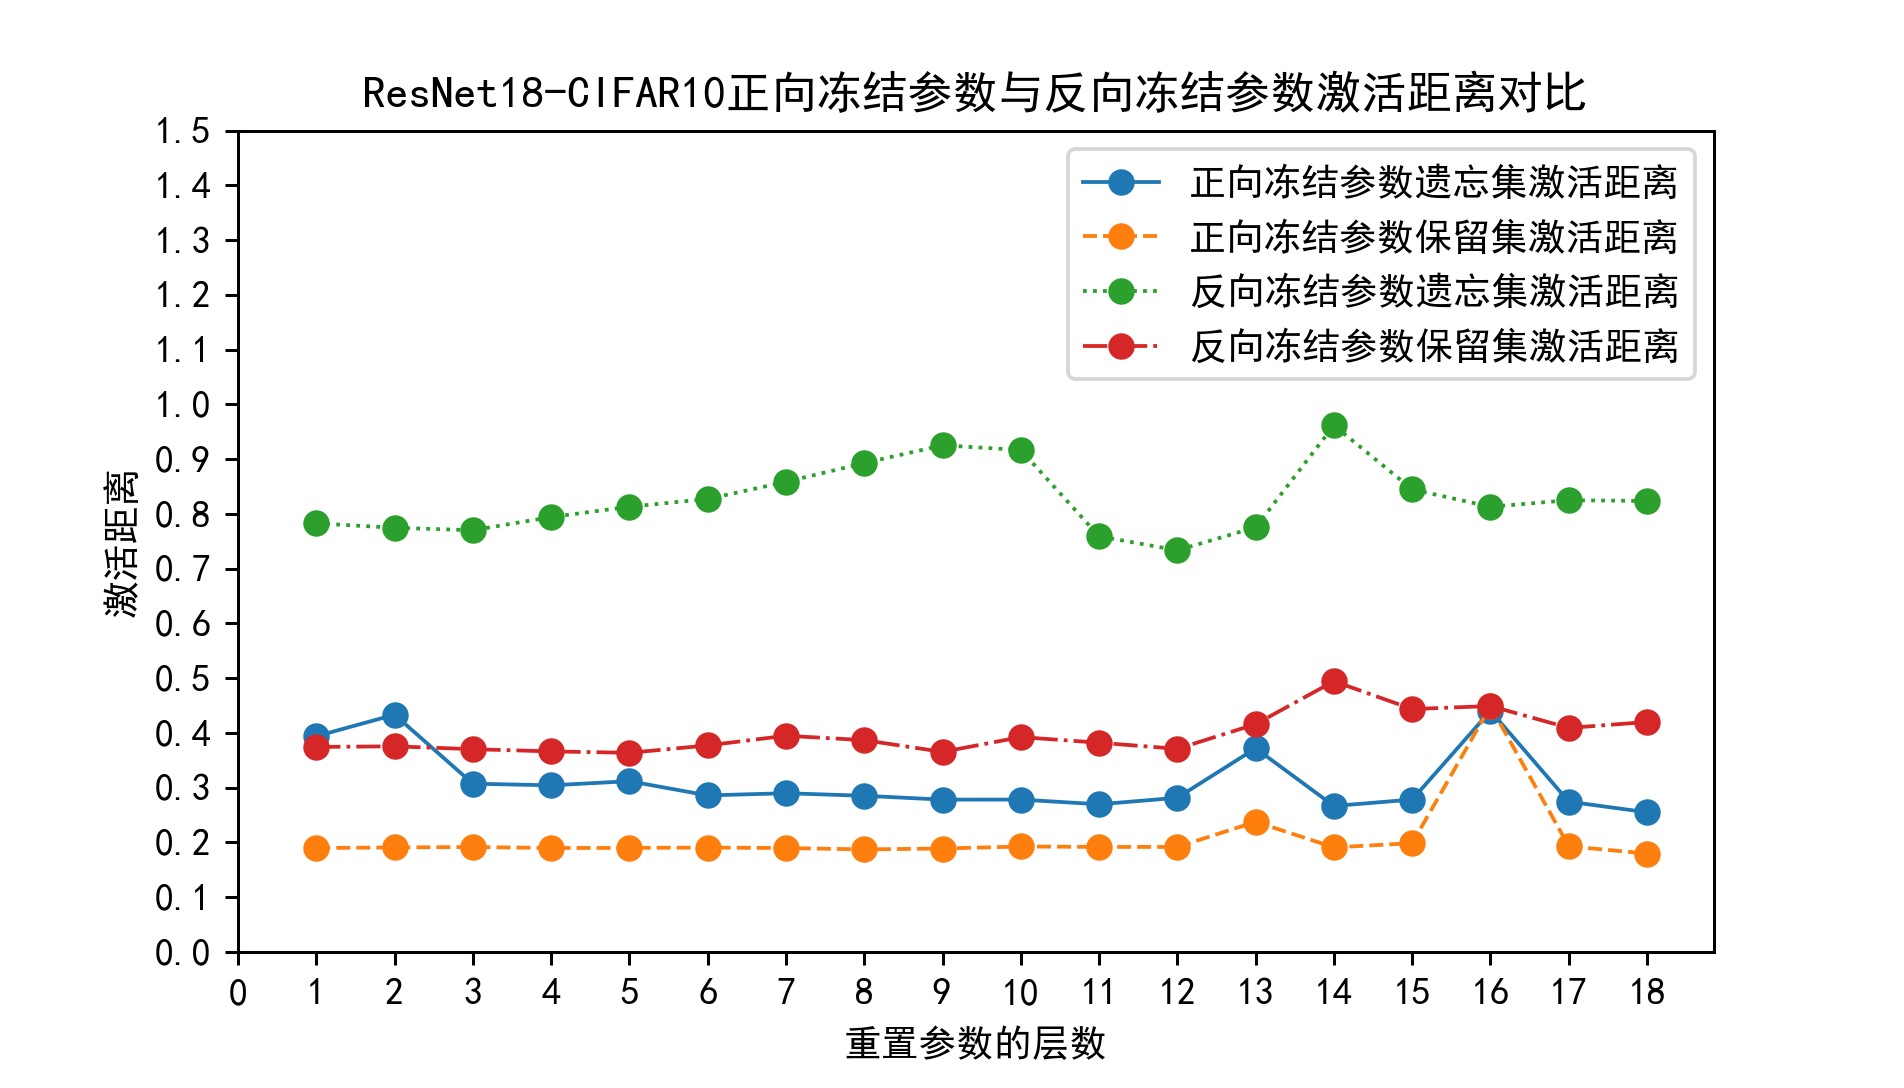
\includegraphics[width=0.9\linewidth]{chapter4_distance_3.png}
    \caption{正向冻结参数与反向冻结参数激活距离对比}
    \label{fig:chapter4_distance_3}
\end{figure}

如图\ref{fig:chapter4_distance_3}所示,图中展示了正向冻结参数与反向冻结参数的情况下,通过保留集去训练网络,再通过遗忘测试集和保留测试集分别测试网络输出距离的对比。
蓝色圆点折线和黄色圆点折线分别代表正向冻结参数的情况下,在遗忘测试集和保留测试集上的网络输出距离的结果。绿色方块折线和红色方块折线分别代表反向冻结参数的情况下,在遗忘测试集和保留测试集上的网络输出距离结果。
从图中可以看出,蓝色圆点折线和黄色圆点折线在激活距离上面从整体上要低于绿色方块折线和红色方块折线。这说明正向冻结参数的方法要好于反向冻结参数的遗忘方法。
\subsection{遗忘可持续性验证实验}
\begin{figure}
    \centering
    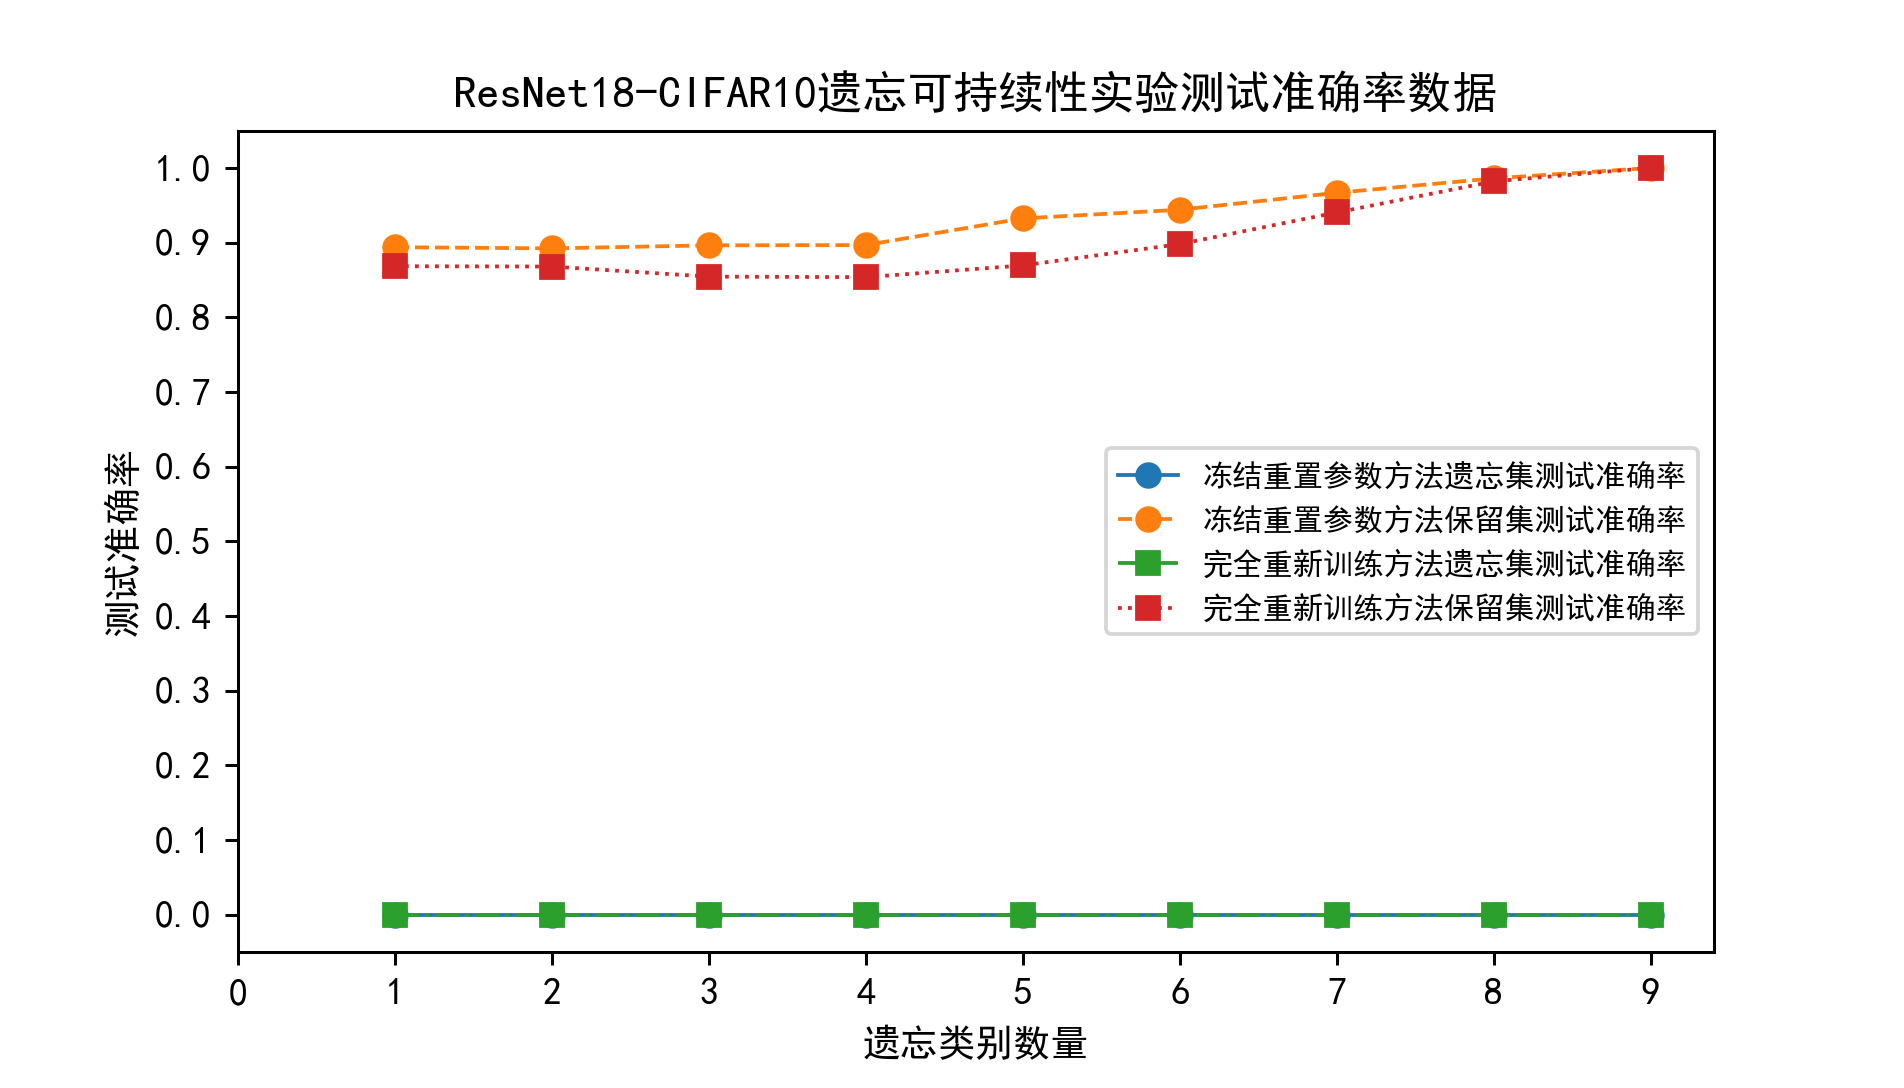
\includegraphics[width=0.9\linewidth]{chapter4_4.png}
    \caption{遗忘可持续性实验测试准确率数据}
    \label{fig:chapter4_4}
\end{figure}

如图\ref{fig:chapter4_4}所示,图中展示了遗忘可持续性实验测试准确率的结果。
图中的横轴代表遗忘类别的数量,本文使用的数据集是CIFAR-10数据集,一共有10个类别,因此遗忘类别的数量最大是9个。图中纵轴则是测试的准确率。
图中蓝色圆点折线和黄色圆点折线分别代表在冻结重置参数方法下在遗忘测试集和保留测试集上的准确率数据。绿色方块折线和红色方块折线分别代表完全重新训练后,在遗忘测试集和保留测试集上得到的准确率数据。
从图中可以看出无论遗忘类别如何变化,遗忘测试集的准确率始终为0,保留集的准确率始终处于较高水平。和完全重新训练相比,冻结重置参数方法在保留集的测试准确率上还略高于完全重新训练的准确率。
这说明无论遗忘掉多少类别,冻结重置参数的方法在测试准确率上均能取得很好效果。

\begin{figure}
    \centering
    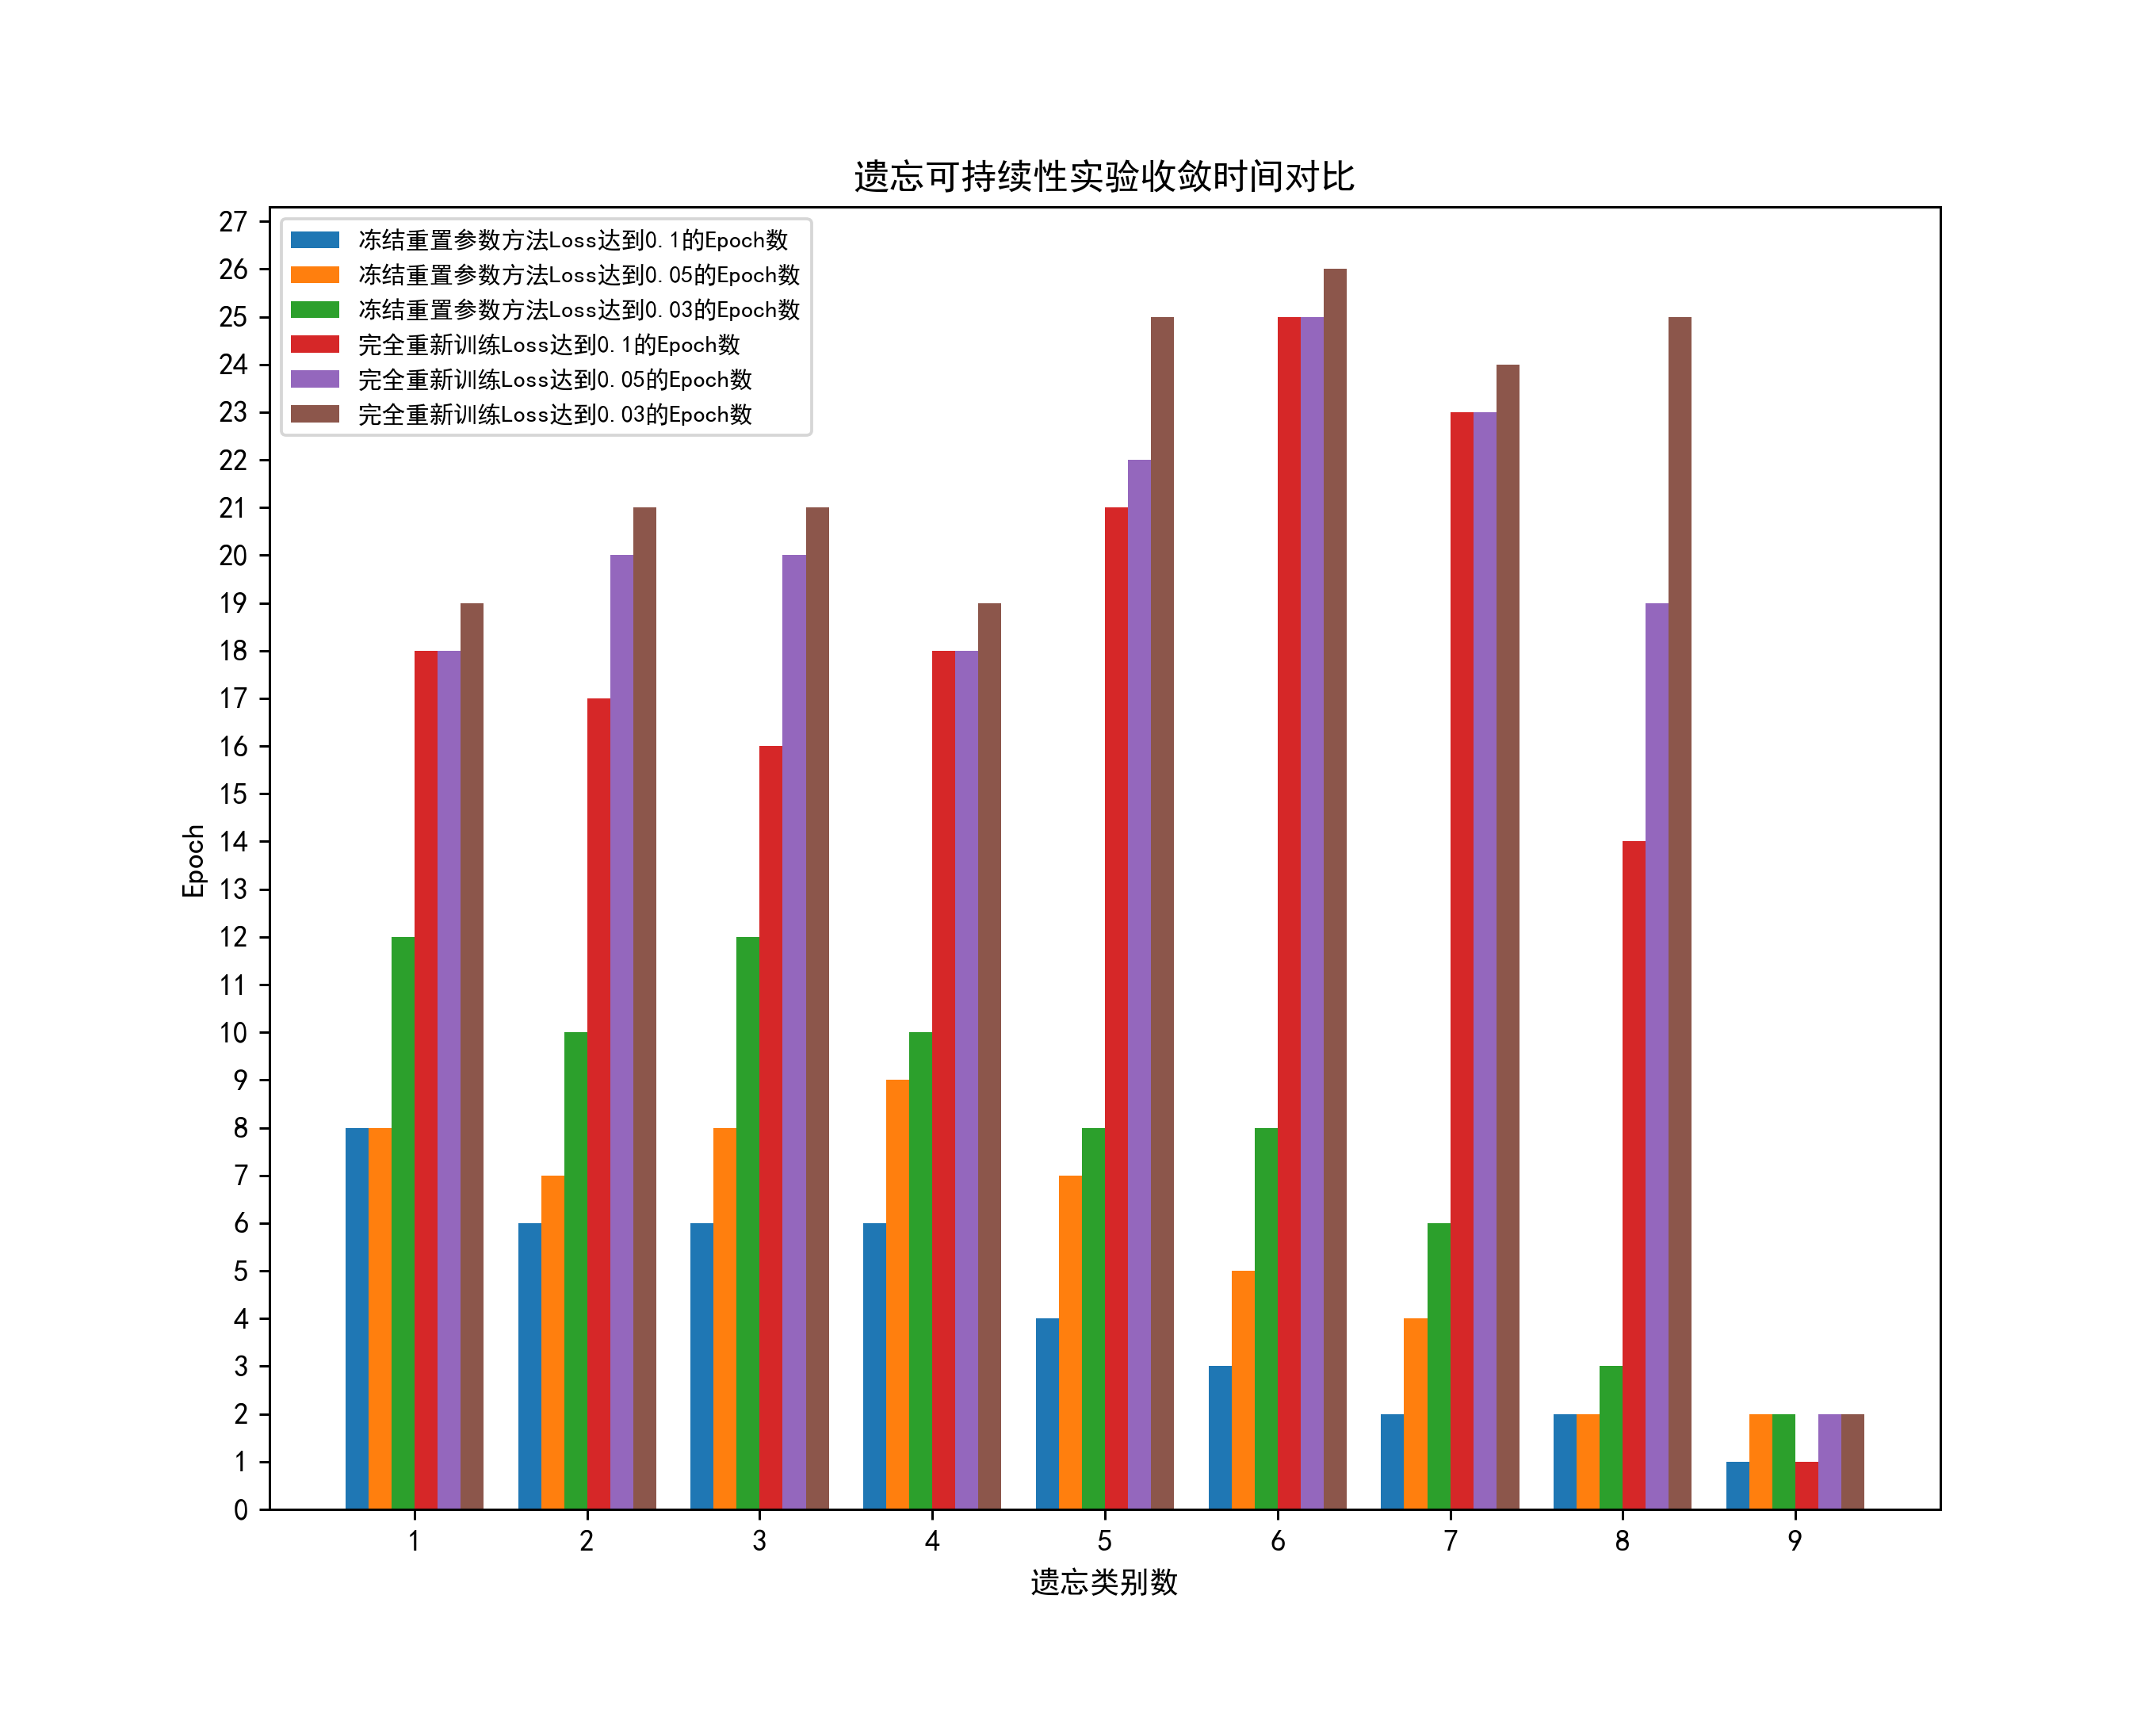
\includegraphics[width=1\linewidth]{chapter4_time_3.png}
    \caption{遗忘可持续性实验收敛时间对比}
    \label{fig:chapter4_time_3}
\end{figure}

如图\ref{fig:chapter4_time_3}所示,图中展示了遗忘可持续性实验不同遗忘类别数下收敛时间的对比情况。
图中横轴是遗忘类别数,纵轴是收敛时间。
图中蓝色、黄色和绿色柱图代表冻结重置参数方法在本文遗忘方法下训练收敛的批次数。红色、紫色和棕色柱图分别代表完全重新训练的收敛批次数。
从图中可以看出,除了遗忘9个类别以外,其余遗忘类别数冻结重置参数方法的收敛时间从整体上要低于完全重新训练的收敛时间。因此无论需要遗忘多少类别,冻结重置参数方法在时间上与完全重新训练相比是节省时间的。

\begin{figure}
    \centering
    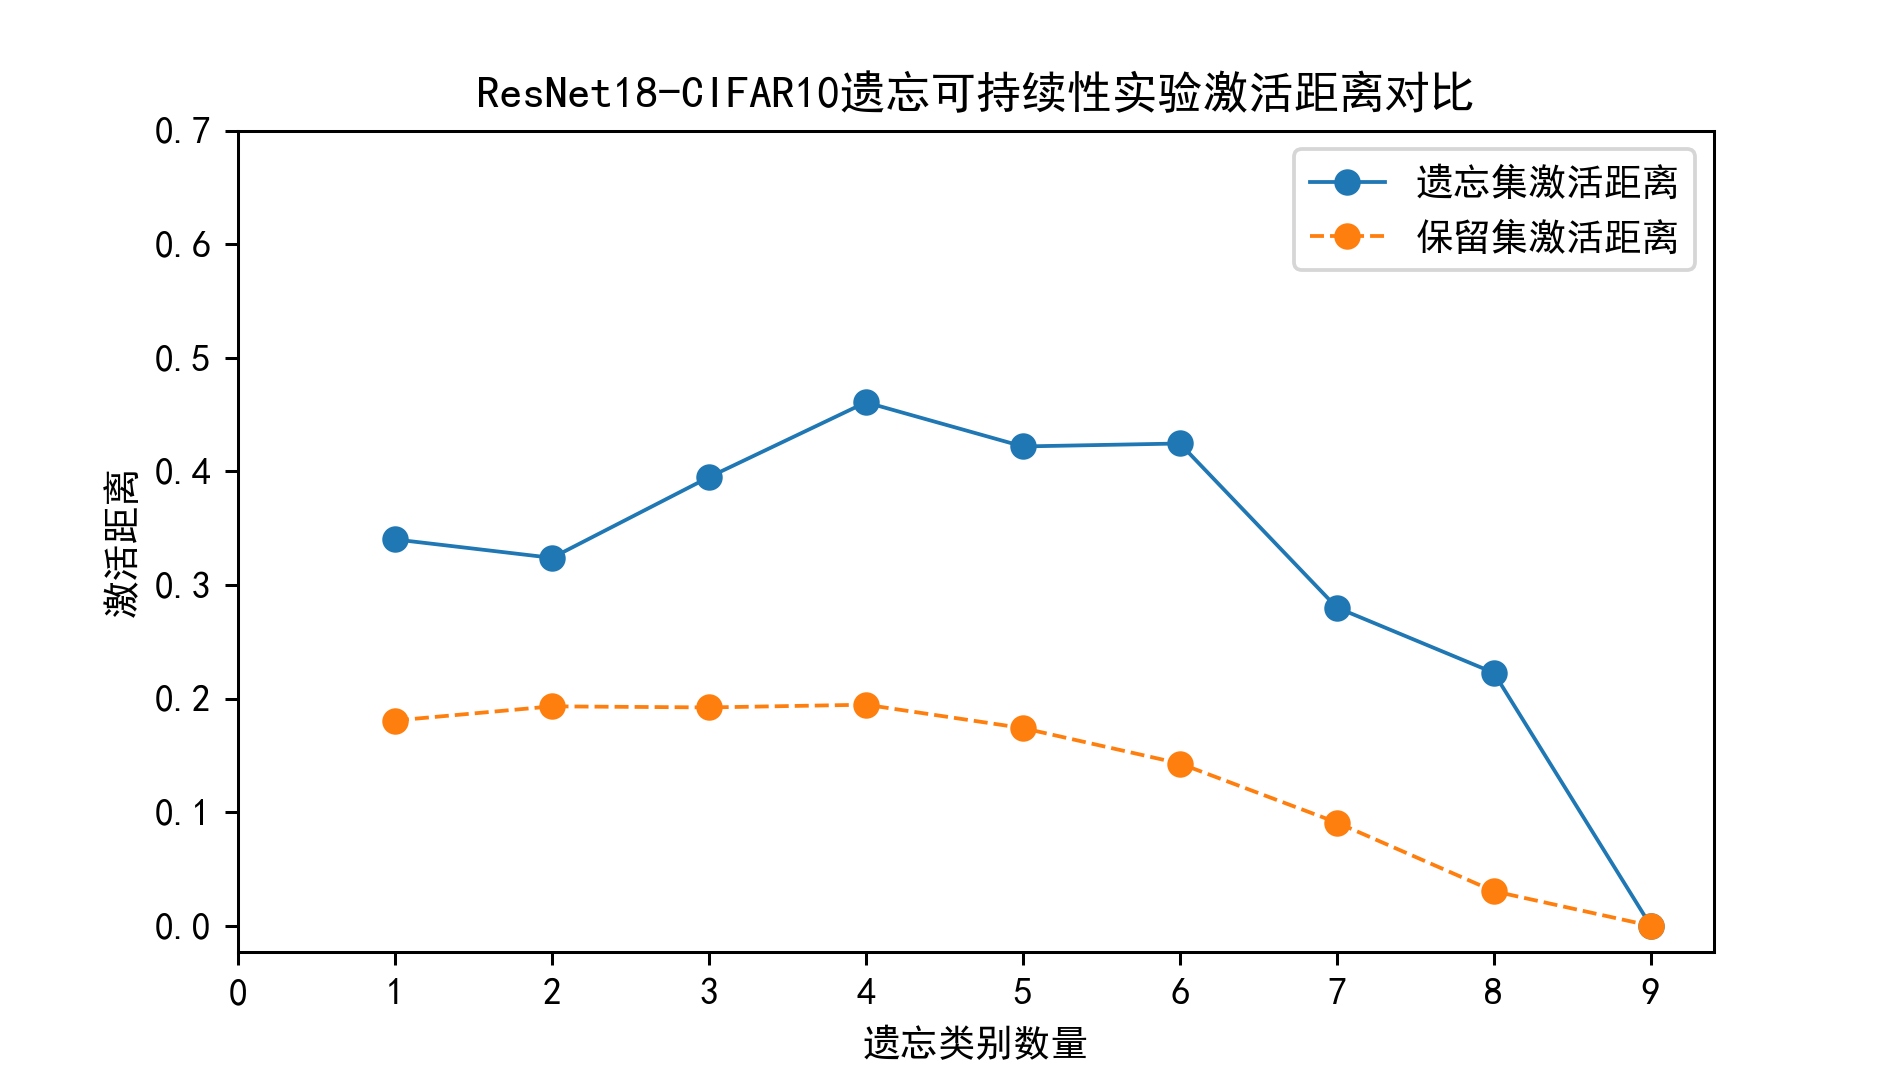
\includegraphics[width=0.9\linewidth]{chapter4_distance_4.png}
    \caption{遗忘可持续性实验激活距离对比}
    \label{fig:chapter4_distance_4}
\end{figure}

如图\ref{fig:chapter4_distance_4}所示,图中展示了遗忘可持续性实验随着遗忘类别的增加激活距离的对比情况。
图中蓝色实线代表经过冻结重置方法遗忘过后的网络,在遗忘测试集上与完全重新训练网络的输出距离。黄色虚线则代表两个网络在保留集上的激活距离。
从图中可以看出,无论是遗忘测试集还是保留测试集,激活距离在整体上是处于较小的数值,这就说明无论遗忘多少类别,本文的遗忘方法与完全重新训练的模型在激活距离上保持得很近。

\section{本章小结}
本章对第三章提出的冻结重置参数的遗忘方法进行了实验验证。首先我们设计了确定重置参数层次的实验。确定的准则通过三个指标来综合考量。
其次,我们设计了冻结和不冻结参数的对比试验,目的是验证冻结参数是有必要的。结果很好地支持了本文提出的方法。
再次,我们设计了反向重置参数与正向重置参数训练的对比试验,其目的是验证卷积神经网络的分层抽象特性,同时也作为正向冻结参数方法的对比实验。
通过反向重置参数的遗忘准确率曲线可以看出,反向重置参数并不能使得遗忘类别达到很好的遗忘效果。而正向重置参数却可以达到很好的遗忘效果,从而验证卷积神经网络的分层抽象特性。
最后为了验证遗忘方法的遗忘可持续性,我们设计了遗忘可持续性实验。通过在准确率、激活距离和收敛时间上面的观察,可以发现无论遗忘类别的数量有多少,冻结重置参数的方法均能达到很好的效果。


% !TeX root = ../thuthesis-example.tex

\chapter{总结与展望}

\section{研究工作总结}

本文通过理论假设和实验验证的方法针对卷积神经网络如何遗忘的问题进行了系统研究。
第一章引言中首先介绍了遗忘问题产生的背景与研究的意义。随着以人脸识别为代表的人工智能技术的广泛应用,越来越多的隐私问题逐渐浮出水面。
研究者发现仅仅通过神经网络的输出数据就能对神经网络模型的输入数据进行还原,或者对神经网络模型训练出来的参数进行抽取,或者能判断出某个输入是否曾经被用于训练该模型。
这些攻击手段的出现给我们发出的一个明显信号就是神经网络模型中包含重要的信息,很可能会由于通过对机器学习模型的攻击而泄露个人隐私数据。这是数据遗忘的用户需求。
从法律角度上看,无论是欧盟出台的GDPR还是美国加州颁布的CCPA,从法律层面上规定了用户拥有“被遗忘权”。当用户需要删除数据时,数据管理者应当及时地履行约定。这是数据需要遗忘的法律要求。
面对这些现实需求,我们研究卷积神经网络的遗忘具有重要的现实意义。
然后,我们介绍了本文设计遗忘方法的主要贡献和本文的文章架构。

在第二章中,本文主要介绍了关于共享网络参数的人工神经网络相关工作和关于机器学习模型遗忘方法的相关工作。
迁移学习的思想和本文的思路在某种程度上是契合的,目的都是无需重新训练整个模型就能够快速地实现模型知识的迁移。
增量学习技术的出发点是克服神经网络本身固有灾难性遗忘。随着新的训练数据继续在网络中训练,原先已经训练过的类别在准确率上有不同程度的降低。
为了解决这个问题,研究人员尝试了多种在无需重新训练全部模型的情况下,想办法将新的类别加入到原有的网络模型当中的方法。其中一类方法就是共享网络参数的方法。
这种方法虽然有网络规模不断扩大的缺点,但是其共享网络参数的思想对本文具有借鉴意义。
在遗忘学习的研究方面,可以大致分为两个类别,一个是基于非神经网络的遗忘方法,这类方法虽然有时可以取得很好的效果,但是面对神经网络时却不能适用。
另一个基于神经网络的遗忘方法。研究者使用了各种方法来尝试还原网络参数,有的通过在权重上增加噪音,有的通过牛顿更新的方法去更新权重。但目前在卷积神经网络的遗忘方面尚没有一套成熟的解决方案。

第三章是本文的核心章节,在第三章为了让读者更好地理解卷积神经网络的分层抽象特性,我们首先介绍了卷积神经网络基本结构和原理。接着介绍了生物视觉信息处理的特点。
然后介绍了卷积神经网络的分层抽象特性。从这个特性出发我们设计了一套遗忘方法,方法可以分为三个步骤:首先确定分层的数值,然后重置并冻结参数,最后使用保留训练集进行训练,直至模型收敛。
我们为了测试遗忘的效果,选取了三个不同方面的测试指标,分别是测试准确率,收敛时间和激活距离。

第四章是对第三章遗忘方法的实验验证。我们设计了四个实验来进行验证,分别是确定冻结层数实验,冻结必要性验证实验,反向冻结验证实验和遗忘可持续性验证实验。确定冻结层数实验,目的是确定冻结参数的层次。
实验结果表明,对于ResNet18的网络结构来说,重置倒数6个层次的参数是个很好的选择。
冻结必要性实验的目的是验证对网络进行冻结的必要性。实验中设计了一套对比实验,通过三个指标的对比表明,冻结参数对提高遗忘效果是有必要的。
反向冻结实验作为本文遗忘方法的一个对照实验,同时也用来验证分层抽象特性的有效性。从实验结果来看,分层抽象特性的效果是明显的。
最后一个实验是遗忘可持续性验证实验,这个实验旨在探究本文提到的遗忘方法是否能够用来连续进行遗忘操作。最终实验结果表明,无论需要遗忘多少类别,本方法均可以达到理想的遗忘效果。

\section{存在问题与展望}
在机器学习模型会泄露个人隐私的背景下,本文对卷积神经网络模型的遗忘方法进行了研究。本文虽然在一定的范围内取得了很好的效果,但是仍有以下几点不足。

第一,本文只能适用于卷积神经网络。通用的机器学习遗忘方法还有待进一步探索和研究。

第二,本方法只能针对保留数据集的情况下使用。有一些实际情况是训练数据不是实时可用,这就导致重置网络参数后无法恢复保留类别原有的准确率。如何不用保留数据集就能实现很好的遗忘效果是一个值得后续研究的方向。

第三,本方法只适用于遗忘整个类别的情况,对于遗忘单个数据的操作,本方法不能做到很好地支持。作者认为有一些数据一旦被用于学习以后,其影响是无法消除的,因此无法被遗忘,有一些相关工作\cite{2018arXiv181205159T}的结论也支持这一点。

\section{本章小结}
本章对全文进行了概括性的总结并对本文目前尚未做到的工作进行了说明,同时又进行了一定的展望。随着卷积神经网络的普遍应用,用户隐私越来越受到重视,基于卷积神经网络的遗忘方法的相关研究势在必行。
% \input{data/chap06}
%\input{data/chap07}
% \input{data/chap08}

% 其他部分
\backmatter

% 参考文献
\bibliography{ref/refs}  % 参考文献使用 BibTeX 编译
% \printbibliography       % 参考文献使用 BibLaTeX 编译

% 附录
\appendix
% % !TeX root = ../thuthesis-example.tex

\begin{survey}
\label{cha:survey}

\title{Title of the Survey}
\maketitle


\tableofcontents


本科生的外文资料调研阅读报告。


\section{Figures and Tables}

\subsection{Figures}

An example figure in appendix (Figure~\ref{fig:appendix-survey-figure}).

\begin{figure}
  \centering
  
\includegraphics[width=0.6\linewidth]{example-image-a.pdf}
  \caption{Example figure in appendix}
  \label{fig:appendix-survey-figure}
\end{figure}


\subsection{Tables}

An example table in appendix (Table~\ref{tab:appendix-survey-table}).

\begin{table}
  \centering
  \caption{Example table in appendix}
  \begin{tabular}{ll}
    \toprule
    File name       & Description                                         \\
    \midrule
    thuthesis.dtx   & The source file including documentaion and comments \\
    thuthesis.cls   & The template file                                   \\
    thuthesis-*.bst & BibTeX styles                                       \\
    thuthesis-*.bbx & BibLaTeX styles for bibliographies                  \\
    thuthesis-*.cbx & BibLaTeX styles for citations                       \\
    \bottomrule
  \end{tabular}
  \label{tab:appendix-survey-table}
\end{table}


\section{Equations}

An example equation in appendix (Equation~\eqref{eq:appendix-survey-equation}).
\begin{equation}
  \frac{1}{2 \uppi \symup{i}} \int_\gamma f = \sum_{k=1}^m n(\gamma; a_k) \mathscr{R}(f; a_k)
  \label{eq:appendix-survey-equation}
\end{equation}


\section{Citations}

Example citations in appendix.
\cite{abrahams99tex}
\cite{salomon1995advanced}
\cite{abrahams99tex,salomon1995advanced}


\bibliographystyle{unsrtnat}
\bibliography{ref/appendix}

\end{survey}
       % 本科生:外文资料的调研阅读报告
% % !TeX root = ../thuthesis-example.tex

\begin{translation}
\label{cha:translation}

\title{书面翻译题目}
\maketitle

\tableofcontents


本科生的外文资料书面翻译。


\section{图表示例}

\subsection{图}

附录中的图片示例(图~\ref{fig:appendix-translation-figure})。

\begin{figure}
  \centering
  
\includegraphics[width=0.6\linewidth]{example-image-a.pdf}
  \caption{附录中的图片示例}
  \label{fig:appendix-translation-figure}
\end{figure}


\subsection{表格}

附录中的表格示例(表~\ref{tab:appendix-translation-table})。

\begin{table}
  \centering
  \caption{附录中的表格示例}
  \begin{tabular}{ll}
    \toprule
    文件名          & 描述                         \\
    \midrule
    thuthesis.dtx   & 模板的源文件,包括文档和注释 \\
    thuthesis.cls   & 模板文件                     \\
    thuthesis-*.bst & BibTeX 参考文献表样式文件    \\
    thuthesis-*.bbx & BibLaTeX 参考文献表样式文件  \\
    thuthesis-*.cbx & BibLaTeX 引用样式文件        \\
    \bottomrule
  \end{tabular}
  \label{tab:appendix-translation-table}
\end{table}


\section{数学公式}

附录中的数学公式示例(公式~\eqref{eq:appendix-translation-equation})。
\begin{equation}
  \frac{1}{2 \uppi \symup{i}} \int_\gamma f = \sum_{k=1}^m n(\gamma; a_k) \mathscr{R}(f; a_k)
  \label{eq:appendix-translation-equation}
\end{equation}


\section{文献引用}

文献引用示例\cite{abrahams99tex}。


% 书面翻译的参考文献
\bibliographystyle{unsrtnat}
\bibliography{ref/appendix}

% 书面翻译对应的原文索引
\begin{translation-index}
  \nocite{salomon1995advanced}
  \bibliographystyle{unsrtnat}
  \bibliography{ref/appendix}
\end{translation-index}

\end{translation}
  % 本科生:外文资料的书面翻译
% % !TeX root = ../thuthesis-example.tex

\chapter{补充内容}

附录是与论文内容密切相关、但编入正文又影响整篇论文编排的条理和逻辑性的资料,例如某些重要的数据表格、计算程序、统计表等,是论文主体的补充内容,可根据需要设置。


\section{图表示例}

\subsection{图}

附录中的图片示例(图~\ref{fig:appendix-figure})。

\begin{figure}
  \centering
  
\includegraphics[width=0.6\linewidth]{example-image-a.pdf}
  \caption{附录中的图片示例}
  \label{fig:appendix-figure}
\end{figure}


\subsection{表格}

附录中的表格示例(表~\ref{tab:appendix-table})。

\begin{table}
  \centering
  \caption{附录中的表格示例}
  \begin{tabular}{ll}
    \toprule
    文件名          & 描述                         \\
    \midrule
    thuthesis.dtx   & 模板的源文件,包括文档和注释 \\
    thuthesis.cls   & 模板文件                     \\
    thuthesis-*.bst & BibTeX 参考文献表样式文件    \\
    thuthesis-*.bbx & BibLaTeX 参考文献表样式文件  \\
    thuthesis-*.cbx & BibLaTeX 引用样式文件        \\
    \bottomrule
  \end{tabular}
  \label{tab:appendix-table}
\end{table}


\section{数学公式}

附录中的数学公式示例(公式~\eqref{eq:appendix-equation})。
\begin{equation}
  \frac{1}{2 \uppi \symup{i}} \int_\gamma f = \sum_{k=1}^m n(\gamma; a_k) \mathscr{R}(f; a_k)
  \label{eq:appendix-equation}
\end{equation}


% 致谢
% !TeX root = ../thuthesis-example.tex

\begin{acknowledgements}
  衷心感谢导师刘云浩教授和丁旋助理研究员对本人毕业论文的悉心指导!
  
  在刘老师的指导下,我价值观得到了很大的提升,使我从一个刚进校门的本科毕业生成长为一个具有国际视野,主动掌握科研前沿讯息的研究生,他的言传身教使我终身受益。
  也十分感谢刘老师在本文关键的地方提出的指导意见。
  
  感谢丁旋老师对这篇论文在构思、素材和格式等方面给予的指导和帮助,也十分感谢丁老师为这篇论文的写作营造了一个严谨、自由的课题组环境,提供了非常专业的实验设备。

  感谢段春晖教授在本论文开题时对开题材料的细心审阅。
  
  感谢我的爸爸潘贵州先生、妈妈孙淑娟女士一直以来的加油打气。
  
  感谢杨一诺同学和李茵学姐在实验设备资源紧张时的慷慨礼让。
  
  感谢室友庞在余和刘斌对我在寝室深夜写论文时发出的噪音表示理解和同情。

  感谢刘琛琦同学在精神上的支持,在我最需要找人倾诉时伸出援手。

  最后感谢所有实验室同学,在我情绪低落的时候给予了精神上的鼓励。
\end{acknowledgements}


% 声明
\statement
% 生成的声明页是否要插入页眉和页脚(默认 empty)
% 仅在需要进行电子签名时,才需要打开这一选项
% 插入的扫描声明页总是会生成页眉(研究生)和页脚,不受这一选项影响
% \statement[page-style=plain]
% 将签字扫描后的声明文件 scan-statement.pdf 替换原始页面
% \statement[file=scan-statement.pdf]

% 个人简历、在学期间完成的相关学术成果
% !TeX root = ../thuthesis-example.tex

\begin{resume}

  \section*{个人简历}

  1989 年 8 月 28 日出生于辽宁黑山县。

  2008 年 9 月考入江苏大学汽车与交通工程学院车辆工程专业,2012 年 7 月本科毕业并获得工学学士学位。

  2012 年 7 月进入上海海马汽车研发有限公司工作,在底盘动力部担任自动变速器标定工程师。

  2015 年 10 月进入九州证券股份有限公司工作,在互联网金融部担任后端研发工程师。

  2018 年 9 月通过全国研究生入学统一考试进入清华大学软件学院攻读软件工程专业工程硕士至今。


  \section*{在学期间完成的相关学术成果}
  无。

  % \subsection*{学术论文}

  % \begin{achievements}
  %   \item Yang Y, Ren T L, Zhang L T, et al. Miniature microphone with silicon-based ferroelectric thin films[J]. Integrated Ferroelectrics, 2003, 52:229-235.
  %   \item 杨轶, 张宁欣, 任天令, 等. 硅基铁电微声学器件中薄膜残余应力的研究[J]. 中国机械工程, 2005, 16(14):1289-1291.
  %   \item 杨轶, 张宁欣, 任天令, 等. 集成铁电器件中的关键工艺研究[J]. 仪器仪表学报, 2003, 24(S4):192-193.
  %   \item Yang Y, Ren T L, Zhu Y P, et al. PMUTs for handwriting recognition. In press[J]. (已被Integrated Ferroelectrics录用)
  % \end{achievements}


  % \subsection*{专利}

  % \begin{achievements}
  %   \item 任天令, 杨轶, 朱一平, 等. 硅基铁电微声学传感器畴极化区域控制和电极连接的方法: 中国, CN1602118A[P]. 2005-03-30.
  %   \item Ren T L, Yang Y, Zhu Y P, et al. Piezoelectric micro acoustic sensor based on ferroelectric materials: USA, No.11/215, 102[P]. (美国发明专利申请号.)
  % \end{achievements}

\end{resume}


% 指导教师/指导小组学术评语
% !TeX root = ../thuthesis-example.tex

\begin{comments}
% \begin{comments}[name = {指导小组学术评语}]
% \begin{comments}[name = {Comments from Thesis Supervisor}]
% \begin{comments}[name = {Comments from Thesis Supervision Committee}]

  论文提出了……

\end{comments}


% 答辩委员会决议书
% !TeX root = ../thuthesis-example.tex

\begin{resolution}



\end{resolution}


% 本科生的综合论文训练记录表(扫描版)
% \record{file=scan-record.pdf}

\end{document}
